\documentclass[a4paper,11pt]{memoir}
\chapterstyle{veelo}

\setcounter{secnumdepth}{4}
\setcounter{tocdepth}{3}
\setsecnumdepth{subsubsection}

\usepackage{standalone}
\usepackage{HTBLA}
\usepackage{multirow}
\usepackage{array} 
\usepackage{color}
\usepackage{xcolor}
\usepackage{colortbl}
\usepackage{mathtools}
\usepackage{amssymb}
\usepackage{wasysym}
\usepackage{pdfpages}
\usepackage{subcaption}
\usepackage{caption}
\usepackage{xargs}
\usepackage[ngerman,colorinlistoftodos]{todonotes}
\usepackage[locale=DE,per-mode=symbol]{siunitx}
\usepackage{longtable}
\usepackage[boxed,german]{algorithm2e}
\usepackage{footnote}
\usepackage{listings}
\usepackage{booktabs}
\usepackage{lscape}
\usepackage{tikz}
\usetikzlibrary{shapes.geometric,arrows,positioning,calc}

\makesavenoteenv{tabular}
\makesavenoteenv{table}

% Quellcode-Darstellung (C/C++ und Python)
\lstset{
  basicstyle=\ttfamily\footnotesize,
  numbers=left,
  numberstyle=\tiny\color{gray},
  stepnumber=1,
  numbersep=6pt,
  backgroundcolor=\color{gray!6},
  frame=single,
  rulecolor=\color{gray!40},
  breaklines=true,
  captionpos=b,
  tabsize=4,
  keywordstyle=\color{blue!70!black}\bfseries,
  commentstyle=\color{green!45!black}\itshape,
  stringstyle=\color{red!60!black},
  literate={ö}{{\"o}}1 {ä}{{\"a}}1 {ü}{{\"u}}1 {Ö}{{\"O}}1 {Ä}{{\"A}}1 {Ü}{{\"U}}1 {ß}{{\ss}}1
}

% Autorenvermerk in der Fusszeile (Analog zu den Vorjahresarbeiten der HTL BULME)
\makeevenfoot{headings}{\thepage}{}{\small\textit{\currentchapterauthor}}
\makeoddfoot{headings}{\small\textit{\currentchapterauthor}}{}{\thepage}
\makeevenfoot{plain}{\thepage}{}{\small\textit{\currentchapterauthor}}
\makeoddfoot{plain}{\small\textit{\currentchapterauthor}}{}{\thepage}

% Metadaten aus ABA - Detailansicht
\thesistitle{Self-Driving Robot Experiments\\(Tumbler~v3.0)}
\selectlanguage{ngerman}
\thesisdate{10.04.2027}
\thesislocation{Graz}

\thesiscurriculum{Elektronik und Technische Informatik}
\thesisverfassung{Verfasser}

\thesisauthoreins{Adem Merdzic}
\thesisauthorzwei{Rami Muarrawi}
\thesisauthordrei{Christopher Schieszler}

\thesismatrikelnoeins{[TODO: SKZ Adem]}
\thesismatrikelnozwei{[TODO: SKZ Rami]}
\thesismatrikelnodrei{[TODO: SKZ Christopher]}

\thesisbetreuung{Betreuer}
\thesisbetreins{Prof.~Dipl.-Ing.~Michael Hollegha}

\bibliographystyle{alpha}

\usepackage[toc]{glossaries}
\makeglossaries

\newglossaryentry{adc}{name={ADC},description={Analog-Digital-Converter -- Analog-Digital-Umsetzer zur Digitalisierung von Sensorspannungen}}
\newglossaryentry{bom}{name={BOM},description={Bill of Materials -- vollständige Stückliste aller elektronischen und mechanischen Komponenten}}
\newglossaryentry{dfam}{name={DfAM},description={Design for Additive Manufacturing -- fertigungsgerechte Konstruktion für den 3D-Druck}}
\newglossaryentry{dmu}{name={DMU},description={Digital Mock-Up -- rechnergestütztes digitales Versuchsmodell zur geometrischen und funktionalen Prüfung einer Baugruppe}}
\newglossaryentry{drc}{name={DRC},description={Design Rule Check -- automatisierte geometrische Leiterplattenprüfung im ECAD-Werkzeug}}
\newglossaryentry{ema}{name={EMA},description={Exponential Moving Average -- exponentiell gewichteter gleitender Mittelwertfilter}}
\newglossaryentry{erc}{name={ERC},description={Electrical Rules Check -- elektrische Plausibilitätsprüfung eines Schaltplans}}
\newglossaryentry{fdm}{name={FDM},description={Fused Deposition Modeling -- additives Fertigungsverfahren durch schichtweises Aufschmelzen eines Thermoplasts}}
\newglossaryentry{fov}{name={FoV},description={Field of View -- optischer Öffnungswinkel bzw. Sichtkegel eines Distanzsensors}}
\newglossaryentry{fsm}{name={FSM},description={Finite State Machine -- endlicher Zustandsautomat zur deterministischen Ablaufsteuerung}}
\newglossaryentry{i2c}{name={I\textsuperscript{2}C},description={Inter-Integrated Circuit -- synchroner, serieller Zweidraht-Datenbus (SDA/SCL) mit Open-Drain-Leitungen}}
\newglossaryentry{imu}{name={IMU},description={Inertial Measurement Unit -- inertiale Messeinheit aus Beschleunigungs- und Drehratensensor}}
\newglossaryentry{lidar}{name={LiDAR},description={Light Detection and Ranging -- optisches Verfahren zur Abstands- und Geschwindigkeitsmessung}}
\newglossaryentry{pcb}{name={PCB},description={Printed Circuit Board -- gedruckte Leiterplatte}}
\newglossaryentry{pid}{name={PID},description={Proportional-Integral-Derivative -- klassischer linearer Regelalgorithmus aus P-, I- und D-Anteil}}
\newglossaryentry{pwm}{name={PWM},description={Pulsweitenmodulation -- Modulationsverfahren zur Leistungs- und Drehzahlregelung}}
\newglossaryentry{rtos}{name={RTOS},description={Real-Time Operating System -- Echtzeitbetriebssystem (hier FreeRTOS) für deterministisches Multitasking}}
\newglossaryentry{ssot}{name={SSOT},description={Single Source of Truth -- eindeutige, zentrale Datenbasis für Konstruktionsparameter}}
\newglossaryentry{tof}{name={ToF},description={Time of Flight -- Laufzeitmessung eines Lichtimpulses zur Distanzbestimmung}}
\newglossaryentry{xshut}{name={XSHUT},description={Active-Low Shutdown-Pin der VL53L0X/VL53L1X-Sensoren zur sequenziellen Adressvergabe}}

\usepackage{hyperref}
\usepackage[figure]{hypcap}
\usepackage{graphicx}

\hypersetup{
  pdftitle   = {Self-Driving Robot Experiments (Tumbler v3.0)},
  pdfsubject = {Diplomarbeit HTL BULME Graz-Goesting},
  pdfauthor  = {Adem Merdzic, Rami Muarrawi, Christopher Schieszler},
  colorlinks = {true},
  linkcolor  = {blue!50!black},
  citecolor  = {green!45!black},
  urlcolor   = {blue!65!black}
}

\begin{document}
\nouppercaseheads
\frontmatter

\newgeometry{left=2.4cm,right=2.4cm,bottom=2.5cm,top=2cm}

\newlength{\tmpbaselineskip}
\setlength{\tmpbaselineskip}{\baselineskip}
\setlength{\baselineskip}{13.6pt}
\newlength{\tmpparindent}
\setlength{\tmpparindent}{\parindent}
\setlength{\parindent}{17pt}

\thispagestyle{tuinftitlepage}
\pagenumbering{Alph}

\begin{center}
\begin{minipage}[t][4.0cm][b]{\linewidth}%
    \centering%
    \thesistitlefontLARGE\sffamily\bfseries\tuinfthesistitle%
\end{minipage}

\vspace{0.9cm}

{\thesistitlefontLARGE\sffamily \tuinfthesistype}

\vspace{5mm}

{\thesistitlefontlarge\sffamily im Rahmen der Fachrichtung}

\vspace{4mm}

{\thesistitlefontLarge\sffamily\bfseries \tuinfthesiscurriculum}

\vspace{6mm}

{\thesistitlefontlarge\sffamily eingereicht von}

\vspace{5mm}

{\thesistitlefontLarge\sffamily\bfseries \tuinfthesisauthoreins} \\
\vspace{1mm}
{\thesistitlefontlarge\sffamily Schülerkennzahl \tuinfthesismatrikelnoeins}

\vspace{4mm}

{\thesistitlefontLarge\sffamily\bfseries \tuinfthesisauthorzwei} \\
\vspace{1mm}
{\thesistitlefontlarge\sffamily Schülerkennzahl \tuinfthesismatrikelnozwei}

\vspace{4mm}

{\thesistitlefontLarge\sffamily\bfseries \tuinfthesisauthordrei} \\
\vspace{1mm}
{\thesistitlefontlarge\sffamily Schülerkennzahl \tuinfthesismatrikelnodrei}

\vspace{1.0cm}

\begin{minipage}[t][1.5cm][t]{\textwidth}%
  \vspace{0pt}\raggedright\thesistitlefontnormalsize\sffamily
  an der

  H\"{o}heren technischen Bundeslehr- und Versuchsanstalt Graz-Gösting
\end{minipage}

\begin{minipage}[t][1.6cm][t]{\textwidth}%
  \vspace{0pt}\sffamily\thesistitlefontnormalsize\raggedright
  Betreuung

  \tuinfthesisbetreuung: \tuinfthesisbetreins
\end{minipage}

\selectlanguage{ngerman}
\begin{minipage}[t][1.6cm][t]{\textwidth}%
  \vspace{0pt}\sffamily\thesistitlefontnormalsize
  \begin{tabbing}%
    \hspace{44mm} \= \hspace{66mm} \= \hspace{51mm} \kill
    Graz, \tuinfthesisdate \> {\raggedright\rule{51mm}{0.5pt}} \> {\raggedright\rule{51mm}{0.5pt}} \\
    \> \begin{minipage}[t][0.5cm][t]{51mm}\centering (Unterschrift \tuinfthesisauthoreins)\end{minipage}
    \> \begin{minipage}[t][0.5cm][t]{51mm}\centering (Unterschrift \tuinfthesisbetreuung)\end{minipage}
  \end{tabbing}
\end{minipage}

\begin{minipage}[t][1.6cm][t]{\textwidth}%
  \vspace{0pt}\sffamily\thesistitlefontnormalsize
  \begin{tabbing}%
    \hspace{44mm} \= \hspace{66mm} \= \hspace{51mm} \kill
    \> {\raggedright\rule{51mm}{0.5pt}} \> {\raggedright\rule{51mm}{0.5pt}} \\
    \> \begin{minipage}[t][0.5cm][t]{51mm}\centering (Unterschrift \tuinfthesisauthorzwei)\end{minipage}
    \> \begin{minipage}[t][0.5cm][t]{51mm}\centering (Unterschrift \tuinfthesisauthordrei)\end{minipage}
  \end{tabbing}
\end{minipage}

\end{center}

\cleardoublepage
\pagenumbering{roman}
\setlength{\baselineskip}{\tmpbaselineskip}
\setlength{\parindent}{\tmpparindent}
\restoregeometry

\textbf{
\begin{center}
Eidesstattliche Erklärung zur Verfassung der Arbeit
\end{center}
}

\noindent
Hiermit erklären wir -- \tuinfthesisauthoreins, \tuinfthesisauthorzwei{} und \tuinfthesisauthordrei{} -- eidesstattlich, dass wir die vorliegende Diplomarbeit selbständig verfasst, keine anderen als die angegebenen Quellen und Hilfsmittel benutzt und die den benutzten Quellen wörtlich oder inhaltlich entnommenen Stellen als solche kenntlich gemacht haben. Diese Arbeit wurde bisher in gleicher oder ähnlicher Form keiner anderen Prüfungsbehörde vorgelegt.

\vspace{1.2cm}
\noindent Graz, am \tuinfthesisdate

\vspace{1.5cm}
\noindent
\begin{tabular}{@{}p{5.2cm}@{\hspace{0.5cm}}p{5.2cm}@{\hspace{0.5cm}}p{5.2cm}@{}}
\dotfill & \dotfill & \dotfill \\
\tuinfthesisauthoreins & \tuinfthesisauthorzwei & \tuinfthesisauthordrei
\end{tabular}


\abstractintoc
\renewcommand{\baselinestretch}{1.15}
\renewcommand{\abstractnamefont}{\normalfont\Large\bfseries}
\renewcommand{\abstractname}{Kurzfassung}
\renewcommand{\abstracttextfont}{\normalsize\nonzeroparskip}
\begin{abstract}
Diese Diplomarbeit dokumentiert die Weiterentwicklung, Neukonstruktion und Systemintegration des autonomen Modellfahrzeugs \emph{Tumbler~v3.0} im Rahmen des Projekts \emph{Self-Driving Robot Experiments} an der HTL BULME Graz-Gösting. Aufbauend auf den Ergebnissen einer vorangegangenen Diplomarbeit wurden zentrale mechanische, schaltungstechnische und softwareseitige Einschränkungen analysiert und durch eine durchgängig neu entwickelte Plattform ersetzt.

Im Hardwarebereich entstand eine zweistufige Elektronikarchitektur rund um den Mikrocontroller \emph{ESP32-S3-WROOM-1}. Für die Spurerkennung wurde eine vollständig neu geroutete, sechskanalige Liniensensor-Platine (\qtyproduct{76 x 32}{\milli\meter}) mit optischen Reflexkopplern (\emph{CNY70}), zwei diskreten Transistor-Stromsenken (\emph{BC817-40}) und RC-Tiefpassfiltern (\qty{1,93}{\kilo\hertz}) entwickelt und fehlerfrei geprüft (0~ERC-/0~DRC-Meldungen). Parallel dazu wurde das Fahrgestell in zehn iterativen CAD-Stufen bis zur druckfertigen Revision~v10.0 überarbeitet. Das monolithische Unibody-Chassis (\qty{220,8}{\centi\meter\cubed}, 100\,\% wasserdichtes STL-Netz für den Bambu Lab P1S) integriert acht \emph{VL53L0/1XV2}-LiDAR-Sensoren mit kollisionsfreien \qty{25}{\degree}-Sichtkegeln, einen nach oben offenen C-Führungskanal zum Einschieben des verlöteten Hauptschalters, sechzehn M2-Teardrop-Sacklöcher sowie vier verdrehsichere M3-Sechskant-Mutterntaschen.

Auf Seiten der Sensorik und Software wurden eine sequenzielle XSHUT-Initialisierung zur dynamischen I\textsuperscript{2}C-Adressvergabe (\texttt{0x30} bis \texttt{0x37}), ein mehrstufiger Median-/EMA-Filter, ein geometrischer Algorithmus zur Längsparklücken-Vermessung sowie eine deterministische FreeRTOS-Softwarearchitektur mit kaskadierter diskreter PID-Regelung (Clamping Anti-Windup) und einem zustandsbasierten Einparkautomaten konzipiert und in C++ (ESP-IDF) implementiert. Die geometrische, elektrische und kinematische Verifikation bestätigt die Funktionsfähigkeit der Gesamtarchitektur; abschließende Hardware-Labormessungen am fertig bestückten Gesamtfahrzeug sind im Testplan strukturiert vorbereitet.

\end{abstract}
\newpage
\renewcommand{\abstractname}{Abstract}
\begin{abstract}
This diploma thesis presents the redesign and extension of the \emph{Tumbler~v3.0} mobile robot platform at HTL~BULME Graz-Gösting into an autonomous testbed for self-parking experiments. To eliminate wiring faults and mechanical fragility, the previous modular breadboard-style electronics are replaced by a custom four-layer mainboard centered around an \emph{ESP32-S3-WROOM-1} microcontroller, integrating dual \emph{TB67H450FNG} H-bridge motor drivers, an \emph{LSM6DSV} six-axis inertial measurement unit, power-protection circuitry, and USB-C connectivity, alongside a redesigned six-channel \emph{CNY70} optical line-sensor board. Environmental perception is achieved by an array of eight \emph{VL53L0/1XV2} time-of-flight LiDAR sensors embedded into a newly engineered, crash-resistant unibody chassis (Revision~v9.0) verified for zero geometric interference across all 121~CAD bodies. On the software side, raw distance readings are filtered in real time to extract candidate parking spaces by width, depth, and orientation, feeding a state machine and closed-loop motor controller to execute collision-free parking maneuvers.

\end{abstract}
\newpage

\cleardoublepage
\makeatletter
\@openrighttrue
\makeatother

\tableofcontents
\listoffigures
\listoftables
\renewcommand{\lstlistlistingname}{Quellcodeverzeichnis}
\lstlistoflistings

\mainmatter
\nonzeroparskip

\chapterauthor{Adem Merdzic, Rami Muarrawi, Christopher Schieszler}
\chapter{Einleitung und Projektmanagement}
\label{chap:einleitung}

\section{Ausgangssituation und Motivation}
\label{sec:motivation}
Mobile Robotik und Fahrerassistenzsysteme gehören heute zu den zentralen Anwendungsgebieten der Elektronik und technischen Informatik. Während in industriellen Fahrzeugen hochauflösende 3D-Laserscanner, Radarsysteme und mehrkernige Recheneinheiten zum Einsatz kommen, lassen sich die grundlegenden regelungstechnischen, sensorischen und algorithmischen Prinzipien bereits an einem kompakten Modellfahrzeug im Labor nachvollziehen. Genau hier setzt die schulinterne Projektlinie \emph{Tumbler} an der HTL BULME Graz-Gösting an.

In der vorangegangenen Diplomarbeit des Jahrgangs 2025/26 \cite{Kloeckl2026} wurde bereits ein fahrfähiger Prototyp (\emph{Tumbler~v2}) aufgebaut, der grundlegende Fahrfunktionen und erste Linienfolge-Versuche ermöglichte. Bei der kritischen Bestandsaufnahme dieses Vorgängermodells zu Beginn unseres Projekts zeigten sich jedoch mehrere technische Grenzen, die einen zuverlässigen autonomen Einparkbetrieb im Labor verhinderten:

\begin{itemize}
  \item \textbf{Eingeschränkte Umfelderfassung:} Der Vorgänger nutzte einzelne Ultraschallsensoren mit breiter akustischer Schallkeule. Bei schrägen Hinderniskanten (z.\,B. Begrenzungen einer Parklücke) kam es häufig zu Mehrfachreflexionen und ungenauen Kantenübergängen. Eine lückenlose \qty{360}{\degree}-Rundumsicht war damit nicht erreichbar.
  \item \textbf{Mechanische Engstellen und Wartbarkeit:} Das bisherige 3D-gedruckte Fahrgestell bot zu wenig Einbauraum für eine geordnete Verkabelung. Insbesondere bei gesteckten Dupont-Verbindern, beim Einbau des 2S-Akkupacks sowie beim seitlichen Hauptschalter fehlten definierte Freiräume und Montagepfade.
  \item \textbf{Schaltungstechnische Altlasten:} Auf der älteren Liniensensor-Platine fehlten dokumentierte Dimensionierungen für die IR-Stromversorgung sowie eine definierte Begrenzung der analogen Ausgangsspannung auf den kalibrierten Messbereich des ESP32-S3-ADCs (\qty{2,9}{\volt}). Zudem waren die Anschlüsse über mehrere Einzelstecker verteilt.
  \item \textbf{Software-Struktur:} Eine einfache Hauptschleife (\emph{Super-Loop}) ohne saubere Echtzeit-Trennung zwischen Sensorabfrage, Motorregelung und übergeordneter Fahrlogik stieß bei paralleler Auswertung mehrerer Distanzsensoren rasch an deterministische Grenzen.
\end{itemize}

Aus diesen konkreten Mängeln entstand die Motivation für unser Diplomarbeitsprojekt \emph{Self-Driving Robot Experiments (Tumbler~v3.0)}. Ziel war es nicht, lediglich einzelne Fehler am Bestandsfahrzeug provisorisch auszubessern, sondern eine saubere, nachvollziehbar dokumentierte und mechanisch robuste Plattform zu schaffen, die sowohl selbstständig einparken kann als auch nachfolgenden Jahrgängen als stabile Experimentierbasis dient.

\section{Projektziele und Abgrenzung}
\label{sec:ziele}
Der Funktionsumfang des \emph{Tumbler~v3.0} wurde zu Projektbeginn gemeinsam mit dem Betreuer Prof.~Dipl.-Ing.~Michael Hollegha im Diplomarbeitsantrag festgelegt und gliedert sich in vier Schwerpunkte:

\begin{enumerate}
  \item \textbf{Neukonstruktion der Hardware und Mechanik:} Entwicklung eines 3D-druckbaren, stoßfesten Unibody-Chassis (Revision~v10.0) für den schuleigenen \emph{Bambu Lab P1S}, das alle acht optischen Distanzsensoren, die Hauptplatine, die neu geroutete Liniensensor-Platine, den 2S-Li-Ion-Akkupack, beide Antriebsmotoren sowie den Hauptschalter kollisionsfrei und wartungsfreundlich aufnimmt.
  \item \textbf{360°-Umfelderfassung mittels 8-fach-LiDAR-Array:} Aufbau eines optischen Sensorrings aus acht \emph{VL53L0/1XV2}-Modulen an einem gemeinsamen I\textsuperscript{2}C-Bus mit sequenzieller \gls{xshut}-Adressvergabe, digitaler Messwertfilterung und geometrischer Erkennung von Längsparklücken.
  \item \textbf{Echtzeitfähige Antriebs- und Kursregelung:} Implementierung einer modularen C++-Firmware unter \emph{ESP-IDF} und \emph{FreeRTOS} mit kaskadierter diskreter PID-Drehzahlregelung, Odometrie-Auswertung über Quadratur-Encoder sowie einem zustandsbasierten Einparkautomaten (\gls{fsm}).
  \item \textbf{Verifikation und Reproduzierbarkeit:} Vollständige digitale Absicherung der Mechanik (BRep-Kollisionsprüfung, \qty{25}{\degree}-Sichtkegel-Audit, Montagepfad-Simulation), elektrische Regelprüfungen (ERC/DRC in KiCad) sowie ein strukturierter Labortestplan für das real aufgebaute Fahrzeug.
\end{enumerate}

Bewusst \textbf{abgegrenzt} wurden kamerabasierte Verfahren (Computer Vision / Objekterkennung mittels neuronaler Netze), globale Indoor-Lokalisierungssysteme (UWB, optisches Motion-Capture) sowie der Betrieb im Außenbereich unter direkter Sonneneinstrahlung. Die Infrarot-ToF-Sensoren arbeiten bei \qty{940}{\nano\meter} Wellenlänge und sind für definierte Innenraum- und Laborbedingungen ausgelegt.

\section{Lasten- und Pflichtenheft}
\label{sec:anforderungen}
Um die technischen Teilbereiche eindeutig voneinander abzugrenzen und am Projektende objektiv überprüfen zu können, wurden alle funktionalen und nicht-funktionalen Anforderungen in Tabelle~\ref{tab:anforderungen} mit eindeutigen Kennungen (\texttt{REQ-01} bis \texttt{REQ-20}) und Prioritäten (\textbf{M} = Muss-Kriterium, \textbf{S} = Soll-Kriterium) festgehalten.

\begin{longtable}{@{}p{1.5cm}p{2.3cm}p{8.8cm}c@{}}
\caption{Anforderungskatalog (Lasten- und Pflichtenheft) für den Tumbler~v3.0.}
\label{tab:anforderungen} \\
\toprule
\textbf{ID} & \textbf{Kategorie} & \textbf{Technische Anforderung / Zielwert} & \textbf{Prio} \\
\midrule
\endfirsthead
\toprule
\textbf{ID} & \textbf{Kategorie} & \textbf{Technische Anforderung / Zielwert} & \textbf{Prio} \\
\midrule
\endhead
\bottomrule
\endfoot
REQ-01 & Mechanik & Monolithisches, direkt auf dem Bambu Lab P1S (\qtyproduct{256 x 256}{\milli\meter}) ohne Stützmaterial druckbares Chassis (PLA/PETG, \qty{0,4}{\milli\meter} Düse). & M \\
REQ-02 & Mechanik & Vollständiges Digital Mock-Up (\gls{dmu}) mit \qty{0,000}{\milli\meter\cubed} Volumenkollision zwischen Chassis, Platinen, Sensoren, Steckern, Motoren und Rädern. & M \\
REQ-03 & Mechanik & Mindestens \qty{2,0}{\milli\meter} Restwandstärke um alle Schraubendome; geschlossene Sacklochböden gegen Durchstoßen von Schrauben. & M \\
REQ-04 & Mechanik & Kollisionsfreie Montagepfade für alle 8 LiDAR-Sensoren (inkl. \qty{24}{\milli\meter} Stecker-Freiraum) sowie werkzeugloser Einschub (\emph{Slide-In}) des verlöteten Hauptschalters. & M \\
REQ-05 & Mechanik & Stoßfestigkeit des Front- und Heckbereichs bei einem Aufprall mit \qty{5}{\kilo\meter\per\hour} (\qty{1,39}{\meter\per\second}) mit Sicherheitsfaktor $\mathrm{SF} \ge 3{,}0$. & S \\
REQ-06 & Energie & Spannungsversorgung aus einem 2S-Li-Ion-Akkupack (\qtyrange{6,4}{8,4}{\volt}, \qtyproduct{72 x 39,5 x 19,5}{\milli\meter}) mit mindestens \qty{1,5}{\milli\meter} Einbauspiel umlaufend. & M \\
REQ-07 & Elektronik & Zentraler Mikrocontroller \emph{ESP32-S3-WROOM-1} mit USB-C-Programmier- und Debug-Schnittstelle sowie 10-poligem JST-GH-Anschluss (\texttt{J2}) für den Liniensensor. & M \\
REQ-08 & Elektronik & Sechskanalige Liniensensor-Platine (\qtyproduct{76 x 32}{\milli\meter}) mit \emph{Vishay CNY70}, konstanter IR-Bestromung ($\approx \qty{20}{\milli\ampere}$) und Ausgangsspannung $< \qty{2,9}{\volt}$ (ESP32-S3 ADC1-Grenze). & M \\
REQ-09 & Elektronik & Fehlerfreie Schaltplan- und Layoutprüfung der Liniensensor-Platine (0~ERC-Fehler, 0~DRC-Verletzungen) sowie geprüfte Signal-Netzliste der Hauptplatine Stufe~1. & M \\
REQ-10 & Elektronik & Getrennte Zweikanal-H-Brücken-Ansteuerung (z.\,B. \emph{TB67H450FNG}) für zwei DC-Getriebemotoren \emph{GA37-520} mit Quadratur-Encodern. & M \\
REQ-11 & Sensorik & Lückenlose \qty{360}{\degree}-Umfelderfassung durch acht \emph{VL53L0/1XV2}-Sensoren mit \qty{0}{\percent} Verdeckung der \qty{25}{\degree}-Sichtkegel durch Chassis, Motoren oder Räder. & M \\
REQ-12 & Sensorik & Sequenzielle \gls{xshut}-Initialisierung und eindeutige dynamische I\textsuperscript{2}C-Adressvergabe (\texttt{0x30} bis \texttt{0x37}) ohne Buskonflikte bei Systemstart. & M \\
REQ-13 & Sensorik & Messwertfilterung (Median- und EMA-Filter) zur Unterdrückung von Einzel-Ausreißern und Behandlung ungültiger Messwerte ($\ge \qty{8190}{\milli\meter}$ bzw. Timeout). & M \\
REQ-14 & Sensorik & Geometrische Erkennung von Längsparklücken ab einer Mindestlänge von $L_{\mathrm{L\ddot{u}cke}} \ge \qty{410}{\milli\meter}$ und Tiefe $D_{\mathrm{L\ddot{u}cke}} \ge \qty{210}{\milli\meter}$ während der Vorbeifahrt. & M \\
REQ-15 & Software & Modulare C++-Firmware unter \emph{ESP-IDF} mit \emph{FreeRTOS}-Tasks und klarer Trennung von Sensorik, Regelung und Zustandsautomat. & M \\
REQ-16 & Regelung & Diskrete PID-Drehzahlregelung beider Antriebsräder mit \qty{100}{\hertz} Abtastrate ($T_s = \qty{10}{\milli\second}$) und \emph{Clamping Anti-Windup} gegen Integrator-Sättigung. & M \\
REQ-17 & Regelung & Autonomes Spurfolgen auf einer kontrastreichen schwarzen Linie (\qtyrange{15}{25}{\milli\meter} Breite) mittels gewichteter Schwerpunktberechnung der 6 CNY70-Kanäle. & M \\
REQ-18 & Autonomie & Deterministischer Einpark-Zustandsautomat (\gls{fsm}) mit automatischer Rückwärts-S-Kurve, Ausrichtung in der Parklücke und Kollisionsabbruch bei $d < \qty{60}{\milli\meter}$. & M \\
REQ-19 & Sicherheit & Hardwareseitiger Hauptschalter in der Batteriezuleitung sowie softwareseitiger Watchdog und Not-Aus bei Sensor-Timeout oder Blockierstrom. & M \\
REQ-20 & Doku & Nachvollziehbare Gesamtdokumentation nach HTL-BULME-Standard mit vollständiger Stückliste, Pinbelegung, CAD-/PCB-Nachweisen und Labortestplan. & M \\
\end{longtable}

\section{Projektmanagement und Teamorganisation}
\label{sec:projektmanagement}
Ein 3-Personen-Projekt über ein gesamtes Schuljahr erfordert klare Zuständigkeiten, damit Hardware, Mechanik und Software parallel entstehen können, ohne sich gegenseitig zu blockieren.

\subsection{Teamstruktur und Arbeitspakete}
Die Aufgaben wurden entlang der fachlichen Schwerpunkte auf die drei Projektmitglieder aufgeteilt (Tabelle~\ref{tab:team}). Übergreifende Themen wie die Systemarchitektur, Schnittstellen-Definitionen (Pinbelegung, Koordinatensysteme) und die finale Systemintegration wurden gemeinsam bearbeitet.

\begin{table}[htbp]
\centering
\caption{Teamzusammensetzung und fachliche Verantwortungsbereiche.}
\label{tab:team}
\begin{tabular}{@{}p{3.6cm}p{4.4cm}p{6.2cm}@{}}
\toprule
\textbf{Teammitglied} & \textbf{Hauptverantwortung} & \textbf{Zugeordnete Arbeitspakete} \\
\midrule
\textbf{Christopher Schieszler} & Hardware, Schaltungstechnik, PCB-Design \& Mechanik/CAD & AP2 (Liniensensor-PCB R2), AP3 (Hauptplatine Stufe 1/2), AP4 (Unibody-Chassis v1–v10, DMU \& 3D-Druck) \\
\textbf{Rami Muarrawi} & Sensorik, I\textsuperscript{2}C-Multiplexing \& Umfelderkennung & AP4 (CAD-Integration LiDAR-Pods), AP5 (8× VL53L0X XSHUT-Treiber \& Filterung), AP6 (Parklücken- \& Linienerkennung) \\
\textbf{Adem Merdzic} & Embedded Software, Regelungstechnik \& Autonomie & AP7 (FreeRTOS-Architektur, Odometrie \& PID-Regler), AP8 (Einpark-FSM, Safety \& Gesamtsystem-Integration) \\
\midrule
\textbf{Prof.~Dipl.-Ing.~M.~Hollegha} & Diplomarbeitsbetreuer & Fachliche Begleitung, Meilenstein-Reviews, Laborfreigabe \\
\bottomrule
\end{tabular}
\end{table}

\subsection{Zeitplan und Meilensteine}
Die zeitliche Abfolge der neun Arbeitspakete (AP1 bis AP9) sowie der sechs verbindlichen Meilensteine (M1 bis M6) ist im Gantt-Diagramm in Abbildung~\ref{fig:gantt} dargestellt. Tabelle~\ref{tab:meilensteine} fasst die zugehörigen Lieferergebnisse (\emph{Deliverables}) zusammen.

\begin{figure}[htbp]
  \centering
  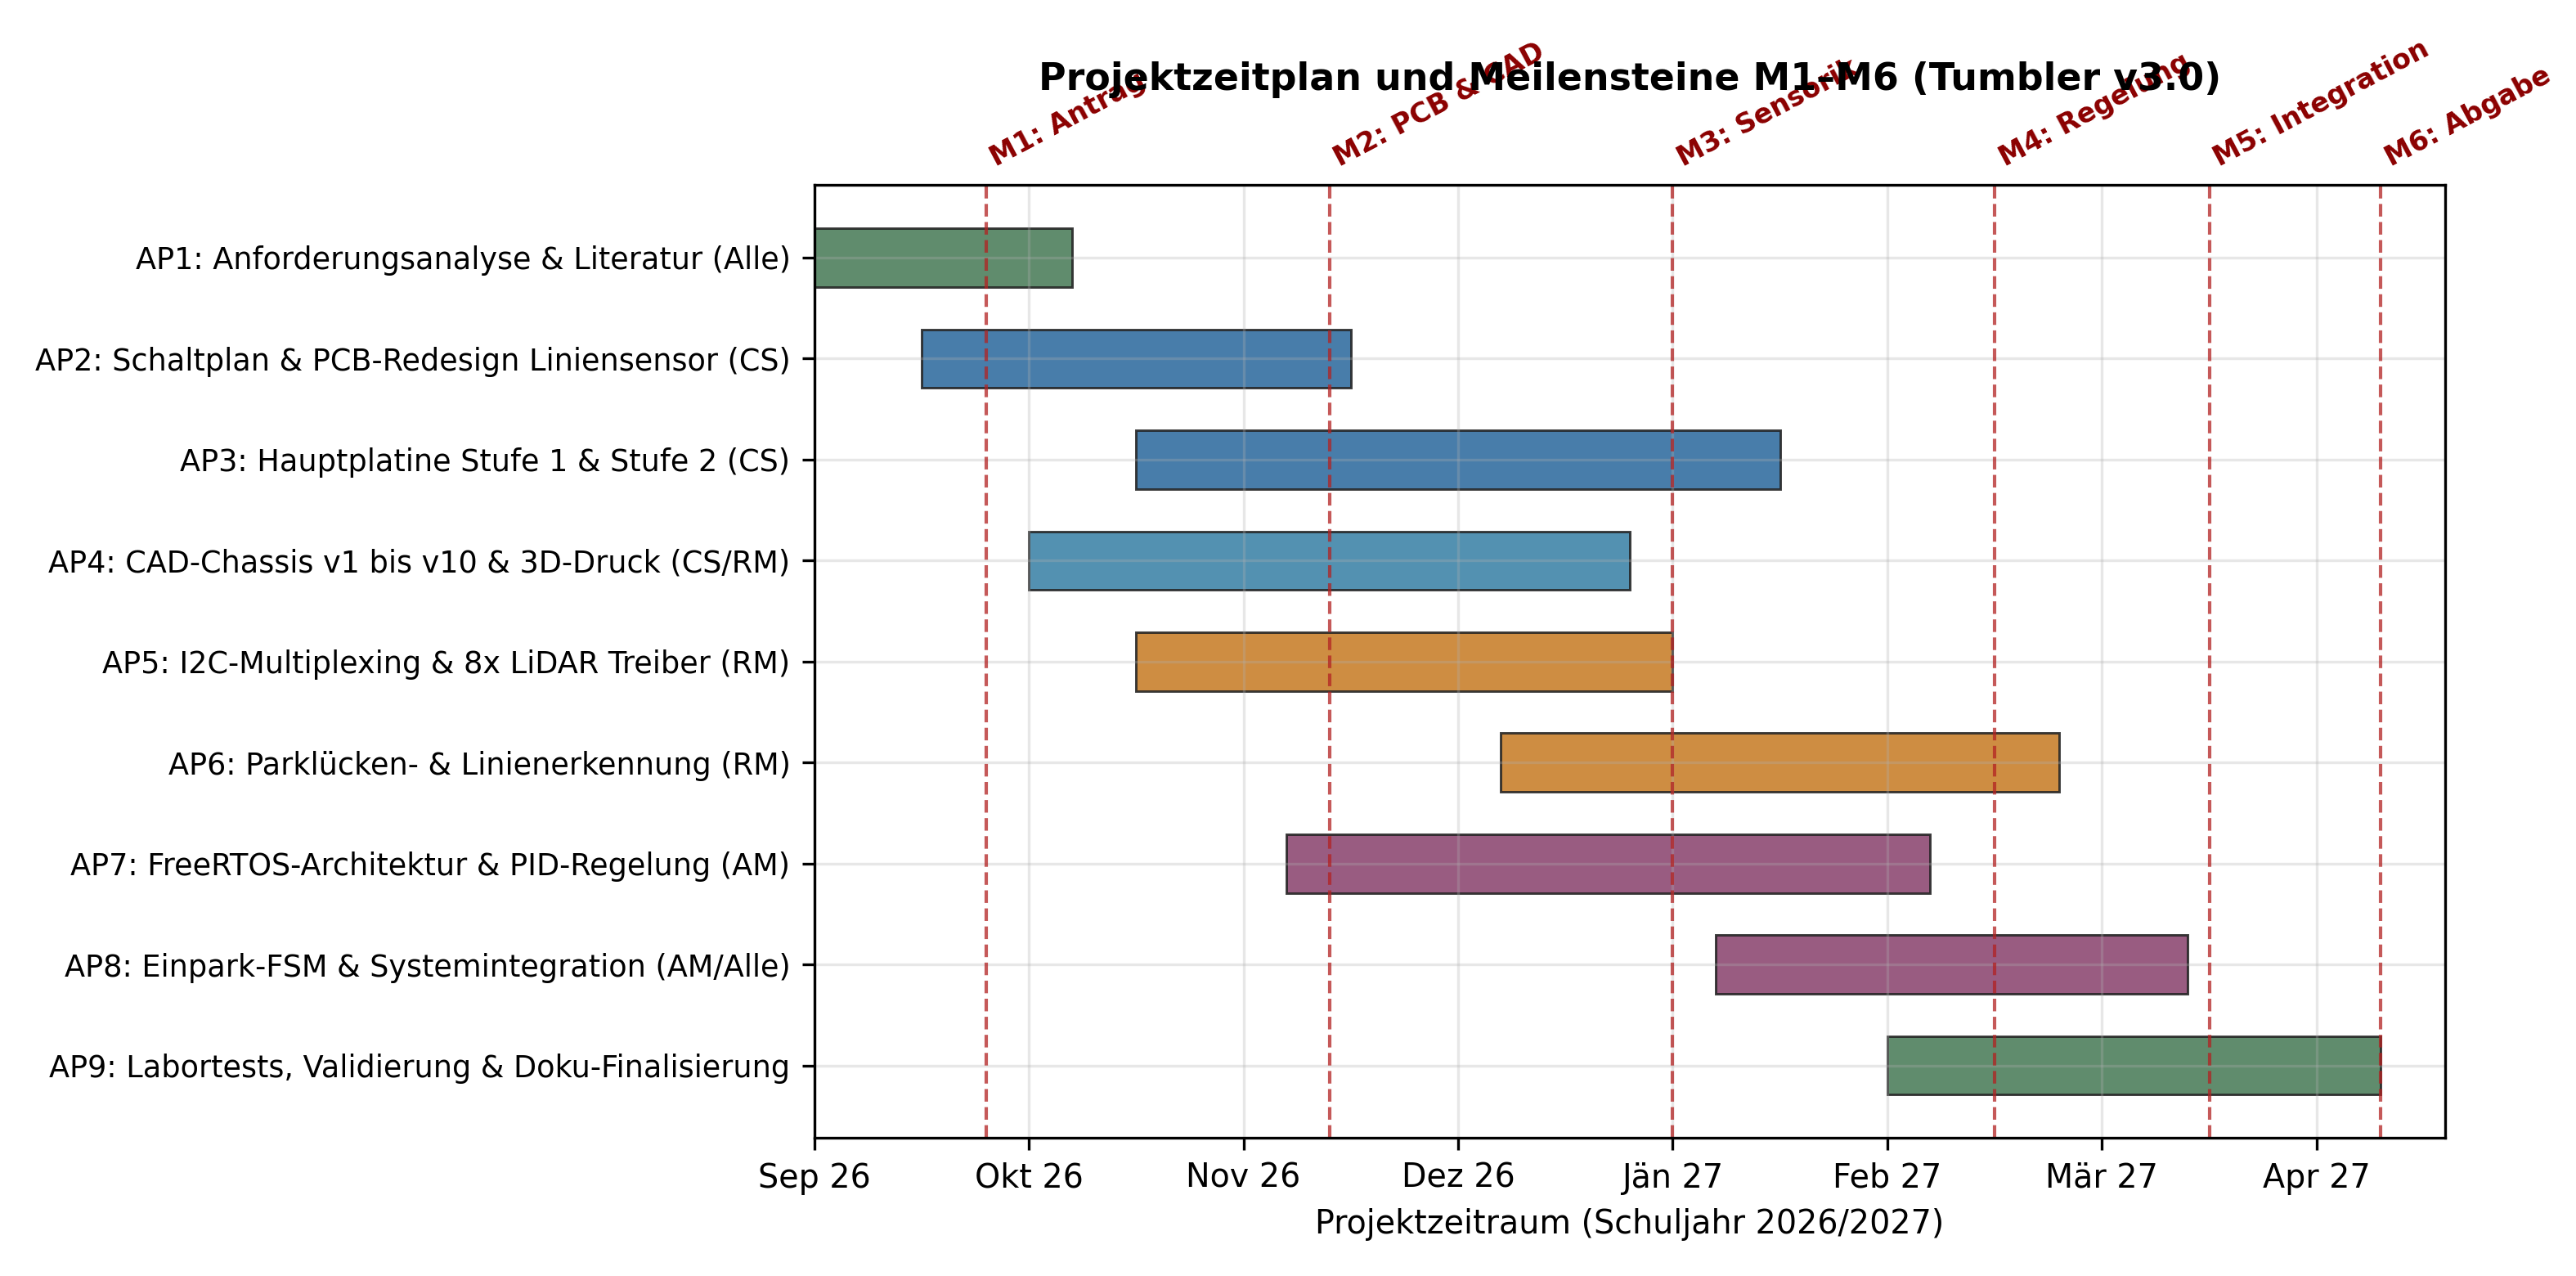
\includegraphics[width=0.98\textwidth]{figures/fig_gantt_milestones.png}
  \caption{Projektzeitplan (Gantt-Diagramm) mit Arbeitspaketen AP1--AP9 und Meilensteinen M1--M6.}
  \label{fig:gantt}
\end{figure}

\begin{table}[htbp]
\centering
\caption{Meilensteinplan M1--M6 gemäß Projektantrag.}
\label{tab:meilensteine}
\begin{tabular}{@{}p{1.2cm}p{2.2cm}p{3.6cm}p{7.2cm}@{}}
\toprule
\textbf{Nr.} & \textbf{Zieltermin} & \textbf{Meilenstein} & \textbf{Abnahmekriterium / Ergebnis} \\
\midrule
M1 & Okt. 2026 & Projektantrag \& Konzept & Freigegebener ABA-Antrag, Lastenheft, Systemarchitektur, Git-Repository eingerichtet. \\
M2 & Nov. 2026 & PCB \& CAD-Freeze & Fehlerfreie Liniensensor-Platine R2 (ERC/DRC = 0), Hauptplatine Stufe 1 geprüft, Chassis v10.0 druckfertig (Watertight STL). \\
M3 & Jän. 2027 & Sensorik-Inbetriebnahme & Alle 8 LiDAR-Sensoren stabil am I\textsuperscript{2}C-Bus (\texttt{0x30}--\texttt{0x37}), CNY70-Kalibrierung im Labor verifiziert. \\
M4 & Feb. 2027 & Regelung \& Spurfolge & Kaskadierter PID-Regler auf dem Fahrzeug abgestimmt, reproduzierbare Linienverfolgung. \\
M5 & Mär. 2027 & Autonomes Einparken & Vollständiger Parkzyklus (Suchen, Vermessen, Rückwärts-Einparken, Stopp) am Testparcours. \\
M6 & Apr. 2027 & Abgabe \& Präsentation & Gebundene Diplomarbeit, Poster, lauffähiger Demonstrator zur Reife- und Diplomprüfung. \\
\bottomrule
\end{tabular}
\end{table}

\subsection{Risikoanalyse und Gegenmaßnahmen}
Bereits in der Konzeptphase wurden die größten technischen und organisatorischen Risiken bewertet (Eintrittswahrscheinlichkeit $W \in \{1..5\}$, Auswirkung $A \in \{1..5\}$, Risikoprioritätszahl $\mathrm{RPZ} = W \cdot A$). Tabelle~\ref{tab:risiko} dokumentiert die abgeleiteten Maßnahmen.

\begin{table}[htbp]
\centering
\caption{Projekt-Risikoanalyse mit konkreten technischen Gegenmaßnahmen.}
\label{tab:risiko}
\begin{tabular}{@{}p{0.9cm}p{3.4cm}ccc p{7.0cm}@{}}
\toprule
\textbf{ID} & \textbf{Risiko} & \textbf{W} & \textbf{A} & \textbf{RPZ} & \textbf{Umgesetzte Gegenmaßnahme} \\
\midrule
R1 & I\textsuperscript{2}C-Buskonflikte oder Blockade bei 8 Sensoren & 4 & 4 & 16 & Sequenzielle \gls{xshut}-Initialisierung mit Hi-Z-Freigabe, \qty{500}{\milli\second} Software-Timeout und sauberer Bus-Pull-up-Auslegung. \\
R2 & Mechanische Kollisionen / unpassender 3D-Druck & 4 & 4 & 16 & Vollständiges 127-Körper-\gls{dmu} mit automatisierter BRep-Kollisionsprüfung (\qty{0,000}{\milli\meter\cubed}), Montagepfad-Checks und Watertight-STL-Test vor dem Druck. \\
R3 & Störeinkopplung der DC-Motoren auf CNY70 / ADC & 3 & 4 & 12 & Durchgehende GND-Fläche, getrennte Masseführung für LED-Stromsenken, \qty{10}{\nano\farad}-RC-Tiefpass je Kanal ($f_g = \qty{1,93}{\kilo\hertz}$) und \qty{100}{\ohm}-Serienwiderstände. \\
R4 & Überschreitung der ADC1-Grenze (\qty{2,9}{\volt}) & 2 & 4 & 8 & Auslegung des Ausgangs-Spannungsteilers (\qty{10}{\kilo\ohm} / \qty{47}{\kilo\ohm}) auf nominal \qty{2,72}{\volt} (Worst-Case \qty{2,87}{\volt} $< \qty{2,9}{\volt}$). \\
R5 & Lieferverzögerungen bei Platinen / Bauteilen & 3 & 3 & 9 & Frühzeitige Standardbauteil-Wahl (0805/1206, gängige MPNs) und Aufbau eines 4-Sensor-Breadboard-Prüfstands für parallele Firmware-Entwicklung. \\
\bottomrule
\end{tabular}
\end{table}

\subsection{Versionsverwaltung und Git-Workflow}
Sämtliche Projektdateien (KiCad-Schaltpläne, CAD-Modelle, ESP-IDF-Quellcode und diese LaTeX-Diplomarbeit) werden zentral im GitHub-Repository \texttt{chrisitrisi/SelfDrivingRobotExperiments} verwaltet. Um Merge-Konflikte zwischen binären CAD-/PCB-Dateien und Textquellen zu vermeiden, arbeiten wir mit dedizierten Themen-Branches:

\begin{itemize}
  \item \texttt{3D\_Design}: Parametrische Python-CAD-Skripte, STEP-/STL-Fertigungsdateien und DMU-Vorschaubilder (aktueller Stand: Revision~v10.0).
  \item \texttt{PCB}: KiCad-Projekte für den Liniensensor (\texttt{Liniensensor\_Redesign}) sowie die Hauptplatine (\texttt{Tumbler\_Stage1}), Gerber-Daten, Stücklisten und ERC-/DRC-Berichte.
  \item \texttt{Main\_code}: ESP-IDF-Firmware-Projekt in C++ inklusive der Portierung der \emph{VL53L0X}-Komponente.
  \item \texttt{Dokumentation}: LaTeX-Quellen, Abbildungen, Literaturdatenbank, Antrag und Präsentationsunterlagen.
\end{itemize}

In der Praxis zeigte sich bei großen Projektarchiven (über \qty{100}{\mebi\byte} bei gepackten ZIP-Dateien), dass GitHub entsprechende Pushes ablehnt. Durch eine gezielte \texttt{.gitignore}-Konfiguration für komprimierte Archive (\texttt{*.zip}, \texttt{*.7z}) und temporäre LaTeX-Hilfsdateien (\texttt{*.aux}, \texttt{*.log}, \texttt{*.toc}) bleibt das Repository schlank und jederzeit reproduzierbar synchronisierbar.

\chapterauthor{Adem Merdzic, Rami Muarrawi, Christopher Schieszler}
\chapter{Systemarchitektur und theoretische Grundlagen}
\label{chap:systemarchitektur}

\section{Gesamtsystem-Übersicht}
\label{sec:gesamtsystem}

Das Fahrzeug folgt einer klaren mechatronischen Schichtenarchitektur, die Energieversorgung, Aktorik, Sensorik und Recheneinheit auf einer gemeinsamen Plattform zusammenführt. Als zentrales Rechenmodul dient ein \emph{ESP32-S3-WROOM-1} mit Dual-Core-Mikrocontroller, Hardware-\gls{pwm}-Einheiten, mehreren I\textsuperscript{2}C-Schnittstellen sowie integrierter WLAN-/Bluetooth-Konnektivität für Telemetrie und Debugging \cite{EspressifESP32S3}.

\begin{figure}[htbp]
  \centering
  \begin{tikzpicture}[
    node distance=1.1cm and 1.4cm,
    block/.style={rectangle, draw=black!80, fill=blue!6, rounded corners=2pt, minimum width=3.1cm, minimum height=0.95cm, align=center, font=\small},
    pwr/.style={rectangle, draw=black!80, fill=orange!10, rounded corners=2pt, minimum width=3.1cm, minimum height=0.95cm, align=center, font=\small},
    sens/.style={rectangle, draw=black!80, fill=green!8, rounded corners=2pt, minimum width=3.1cm, minimum height=0.95cm, align=center, font=\small},
    arrow/.style={->, >=stealth, thick}
  ]
    \node[block] (mcu) {\textbf{ESP32-S3-WROOM-1}\\Hauptsteuerung (U3)};
    \node[pwr, above=of mcu] (pwr) {\textbf{Power Management}\\2S Li-Ion, 5\,A-Sicherung,\\AP63203 (3,3\,V) \& AMS1117 (5\,V)};
    \node[sens, left=1.8cm of mcu] (lidar) {\textbf{8x VL53L0/1XV2}\\360\textdegree-LiDAR-Array\\(I\textsuperscript{2}C + XSHUT)};
    \node[sens, below left=1.1cm and 0.6cm of mcu] (line) {\textbf{Liniensensor}\\6x CNY70 + 2x BC817\\(Analog / ADC)};
    \node[sens, below right=1.1cm and 0.6cm of mcu] (imu) {\textbf{6-Achs-IMU}\\LSM6DSV (U5)\\(SPI / I\textsuperscript{2}C)};
    \node[block, right=1.8cm of mcu] (drv) {\textbf{2x TB67H450FNG}\\SMD-H-Brücken (U6, U7)\\\& 2x GA37-520 Motoren};

    \draw[arrow] (pwr) -- (mcu);
    \draw[arrow] (pwr) -| (drv);
    \draw[arrow] (lidar) -- (mcu);
    \draw[arrow] (line) |- (mcu);
    \draw[arrow] (imu) |- (mcu);
    \draw[arrow] (mcu) -- (drv);
  \end{tikzpicture}
  \caption{Blockschaltbild der Gesamtsystemarchitektur des Tumbler~v3.0 (Redesign).}
  \label{fig:blockschaltbild}
\end{figure}

\section{Evolution vom Vorgängermodell zum Redesign}
\label{sec:evolution}

Im Rahmen der Aufgabenanalyse zeigte sich, dass eine reine Software-Erweiterung auf der bestehenden Hardware-Basis nicht zielführend ist. Tabelle~\ref{tab:vergleich_alt_neu} stellt die wesentlichen Änderungen zwischen dem Ausgangszustand (\emph{Tumbler~v3.0} \cite{Kloeckl2026}) und dem vorliegenden Redesign gegenüber.

\begin{table}[htbp]
  \centering
  \caption{Gegenüberstellung der Hardware-Architektur vor und nach dem Redesign.}
  \label{tab:vergleich_alt_neu}
  \begin{tabular}{@{}p{3.6cm}p{5.2cm}p{5.5cm}@{}}
    \toprule
    \textbf{Teilsystem} & \textbf{Ausgangsbasis (Vorgänger)} & \textbf{Redesign (diese Arbeit)} \\
    \midrule
    Motortreiber & Externe Steckmodule über Stiftleisten & Zwei integrierte SMD-ICs (\emph{TB67H450FNG}) direkt auf der Hauptplatine \\
    Inertialsensorik (IMU) & Aufgestecktes Breakout-Board & Direkt bestücktes QFN-Bauteil (\emph{LSM6DSV}) auf der Hauptplatine \\
    Abstandssensorik & Ultraschallsensor / begrenzte Sicht & 8x \emph{VL53L0/1XV2} Time-of-Flight LiDAR in geschützten Pods (360\textdegree) \\
    Liniensensor & Ältere Sensorplatine & Kompaktes \qtyproduct{76 x 32}{\milli\metre} Redesign mit 6x \emph{CNY70} und BC817-Treibern \\
    Chassis & Offene Plattform, geringe Wandstärken & Crashresistentes Unibody-Chassis (Rev.~v9.0), 0\textdegree-Kollision im DMU \\
    \bottomrule
  \end{tabular}
\end{table}

\paragraph{Begründung der 8-fach-LiDAR-Anordnung.}
Während im ursprünglichen Antrag noch allgemein von einem 360\textdegree-LiDAR-Sensor die Rede war, fiel im Systementwurf die Entscheidung auf acht diskrete \emph{VL53L0/1XV2}-Sensoren (drei vorne, zwei seitlich, drei hinten). Diese Lösung vermeidet rotierende mechanische Verschleißteile, baut deutlich flacher, lässt sich direkt in das robuste Unibody-Chassis einbetten und liefert dennoch eine geschlossene Rundum-Abdeckung ohne Totzonen durch Räder oder Motoren.

\section{Verwendete Sensor- und Kommunikationsprinzipien}
\label{sec:grundlagen_sensorik}

\subsection{Time-of-Flight-Abstandsmessung (VL53L0/1XV2)}
Die verwendeten \gls{tof}-Sensoren senden augensichere Infrarot-Laserimpulse (\SI{940}{\nano\metre} VCSEL) aus und bestimmen die Distanz $d$ direkt aus der Laufzeit $\Delta t$ des reflektierten Lichts:
\begin{equation}
  d = \frac{c_0 \cdot \Delta t}{2}
  \label{eq:tof_distanz}
\end{equation}
Dabei bezeichnet $c_0 \approx \SI{2.998e8}{\metre\per\second}$ die Lichtgeschwindigkeit. Im Gegensatz zu klassischen Ultraschallsensoren besitzen \emph{VL53L0X}- und \emph{VL53L1X}-Sensoren einen eng begrenzten Öffnungswinkel (Field of View, FoV) von rund \SI{25}{\degree} \cite{ST_VL53L0X,ST_VL53L1X}, wodurch schmale Parklücken und seitliche Kanten wesentlich präziser aufgelöst werden können.

\subsection{I\textsuperscript{2}C-Bus und Hardware-Adressierung}
Alle \gls{tof}-Module kommunizieren über den zweidrahtigen I\textsuperscript{2}C-Bus (\texttt{SDA}, \texttt{SCL}). Da jeder Sensor ab Werk dieselbe Standardadresse (\texttt{0x29}) besitzt, werden die \texttt{XSHUT}-Eingänge der acht Module getrennt angesteuert. Beim Systemstart werden zunächst alle Sensoren in den Reset-Zustand versetzt und anschließend nacheinander aktiviert, um jedem Baustein eine eindeutige I\textsuperscript{2}C-Adresse zuzuweisen.

\subsection{Inertiale Messeinheit (LSM6DSV) und PWM-Antrieb}
Für die Bestimmung der Fahrzeugdrehung während des Einparkvorgangs integriert die Hauptplatine den 6-Achs-Sensor \emph{LSM6DSV} \cite{ST_LSM6DSV}. Durch Integration der Gierrate $\omega_z(t)$ lässt sich der aktuelle Gierwinkel $\psi(t)$ bestimmen:
\begin{equation}
  \psi(t) = \psi_0 + \int_{t_0}^{t} \left(\omega_z(\tau) - b_z\right)\,\mathrm{d}\tau
  \label{eq:yaw_integration}
\end{equation}
Hierbei berücksichtigt $b_z$ den vor dem Anfahren kalibrierten Nullpunktfehler (Bias) des Gyroskops. Die Ansteuerung der beiden Gleichstrom-Getriebemotoren erfolgt über zwei H-Brücken vom Typ \emph{TB67H450FNG} \cite{Toshiba_TB67H450} mittels \gls{pwm}-Signalen zur stufenlosen Geschwindigkeits- und Richtungsvorgabe.

\chapterauthor{Christopher Schieszler}
\chapter{Hardwareentwicklung, Schaltungstechnik und CAD-Konstruktion}
\label{chap:hardware}

Dieses Kapitel dokumentiert die vollständige elektronische und mechanische Neuentwicklung des \emph{Tumbler~v3.0}. Im ersten Teil werden der Schaltungsentwurf, die exakte Bauteildimensionierung sowie die Layout- und Regelprüfungen (ERC/DRC) der sechskanaligen Liniensensor-Platine und der überarbeiteten Hauptplatine behandelt. Der zweite Teil beschreibt die iterative 3D-CAD-Entwicklung des Unibody-Chassis bis zur druckfertigen Revision~v10.0, inklusive der fertigungsgerechten Auslegung (\gls{dfam}) für den \emph{Bambu Lab P1S}, der mechanischen Stoßfestigkeitsrechnung und der vollständigen Stückliste.

% ==============================================================================
\section{Neuentwicklung der Liniensensor-Platine (Layout R2)}
\label{sec:liniensensor_pcb}
% ==============================================================================
Die ursprünglich vorhandene Liniensensor-Schaltung aus der Vorjahresarbeit \cite{Kloeckl2026} wies mehrere gravierende Mängel auf: Die sechs optischen Reflexkoppler (\emph{CNY70}) waren über vier getrennte Steckverbinder (\texttt{J1}--\texttt{J4}) verdrahtet, es fehlten verbindliche Widerstandswerte für die Strombegrenzung und den Ausgangsteiler, und es existierte kein geprüftes Zweilagen-Layout mit durchgehender Massefläche. Im Rahmen dieser Diplomarbeit entstand daher das vollständig überarbeitete Paket \texttt{Liniensensor\_Redesign} (Schaltung~R1 / Layout~R2 in KiCad~9.0.9).

\subsection{Schaltungstopologie und Dimensionierung der IR-LED-Stromsenken}
Die sechs IR-Sendedioden der Reflexkoppler \texttt{U1}--\texttt{U6} (\emph{Vishay CNY70} \cite{Vishay_CNY70}) werden in zwei symmetrischen Dreier-Reihenschaltungen (\texttt{U1}--\texttt{U3} sowie \texttt{U4}--\texttt{U6}) direkt aus der geschalteten 2S-Akkuschiene \texttt{VBAT\_SW} (\qtyrange{6,4}{8,4}{\volt}) gespeist. Dadurch wird die \qty{3,3}{\volt}-Logikversorgung vollständig entlastet. Um den Diodenstrom trotz sinkender Akkuspannung weitgehend stabil bei rund \qty{20}{\milli\ampere} zu halten, steuert je ein NPN-Transistor \texttt{Q1}/\texttt{Q2} (\emph{Nexperia BC817-40,215}, SOT-23 \cite{Nexperia_BC817}) mit Emitterwiderstand $R_E = R_1 = R_9 = \qty{47}{\ohm}$ (\qty{1}{\percent}, 0805) als einfache Konstantstromsenke den Strangstrom.

Die Basisspannung wird über einen symmetrischen Spannungsteiler aus zwei \qty{1}{\kilo\ohm}-Widerständen (\texttt{R2}/\texttt{R3} bzw. \texttt{R7}/\texttt{R8}) aus den geregelten \qty{3,3}{\volt} gewonnen. Nach dem Satz von Thévenin ergeben sich die Leerlaufspannung $V_{\mathrm{th}}$ und der Innenwiderstand $R_{\mathrm{th}}$ der Basisquelle zu \cite{TietzeSchenk}:
\begin{equation}
  V_{\mathrm{th}} = \frac{\qty{3,3}{\volt}}{2} = \qty{1,65}{\volt}, \qquad
  R_{\mathrm{th}} = \qty{1}{\kilo\ohm} \parallel \qty{1}{\kilo\ohm} = \qty{500}{\ohm}
  \label{eq:ls_thevenin}
\end{equation}
Unter Berücksichtigung der Stromverstärkung $\beta$ und der Basis-Emitter-Flussspannung $V_{BE}$ folgt für den Kollektorstrom $I_C$ (identisch mit dem IR-LED-Strom $I_F$ jeder der drei in Serie liegenden Dioden):
\begin{equation}
  I_C = \frac{V_{\mathrm{th}} - V_{BE}}{R_E \cdot \left(1 + \frac{1}{\beta}\right) + \frac{R_{\mathrm{th}}}{\beta}}
  \label{eq:ls_stromsenke}
\end{equation}
Für typische Werte eines \emph{BC817-40} ($\beta = 200$, $V_{BE} = \qty{0,65}{\volt}$) ergibt sich:
\begin{equation}
  I_C = \frac{\qty{1,65}{\volt} - \qty{0,65}{\volt}}{\qty{47}{\ohm} \cdot 1{,}005 + \frac{\qty{500}{\ohm}}{200}} = \frac{\qty{1,00}{\volt}}{\qty{49,735}{\ohm}} = \qty{20,11}{\milli\ampere}
  \label{eq:ls_ic_nom}
\end{equation}
Bei $V_{BE} = \qty{0,70}{\volt}$ sinkt der Strom geringfügig auf \qty{19,10}{\milli\ampere}. Beide Stränge zusammen entnehmen somit rund \qty{40}{\milli\ampere} aus \texttt{VBAT\_SW} -- weit unter dem absoluten Grenzstrom der CNY70-LED (\qty{50}{\milli\ampere}).

\subsubsection{Verlustleistungs- und Grenzfallanalyse (6,4 V bis 8,4 V)}
Bei voll geladenem 2S-Akku ($U_{\mathrm{Bat}} = \qty{8,4}{\volt}$) und einer typischen IR-LED-Flussspannung von $V_F \approx \qty{1,25}{\volt}$ pro Diode ($3 \times \qty{1,25}{\volt} = \qty{3,75}{\volt}$) verbleibt über Emitterwiderstand und Transistor eine Spannung von $\qty{8,4}{\volt} - \qty{3,75}{\volt} = \qty{4,65}{\volt}$. Die entstehenden Verlustleistungen liegen weit innerhalb der zulässigen Bauteilgrenzen \cite{Vishay_CRCW,Nexperia_BC817}:
\begin{align}
  P_{R1,R9} &= I_E^2 \cdot R_E \approx (\qty{20,2}{\milli\ampere})^2 \cdot \qty{47}{\ohm} = \qty{19,2}{\milli\watt} \quad (\text{Nennwert: } \qty{125}{\milli\watt}) \label{eq:ls_p_re} \\
  P_{Q1,Q2} &= U_{CE} \cdot I_C \approx (\qty{4,65}{\volt} - \qty{0,95}{\volt}) \cdot \qty{20,11}{\milli\ampere} = \qty{74,4}{\milli\watt} \quad (\text{Nennwert: } \qty{250}{\milli\watt}\text{ bei }\qty{25}{\celsius}) \label{eq:ls_p_q}
\end{align}
Selbst in einer konservativen Worst-Case-Parameterstudie (\qty{3,3}{\volt} $\pm 5\,\%$, Widerstände $\pm 1\,\%$, $\beta \in [100, 600]$, $V_{BE} \in [\qty{0,5}{\volt}, \qty{0,9}{\volt}]$, $V_F \in [\qty{0,9}{\volt}, \qty{1,6}{\volt}]$) bleibt der Strangstrom im Bereich \qtyrange{12,3}{26,3}{\milli\ampere} und die maximale Transistorverlustleistung bei \qty{117,8}{\milli\watt} (bei \qty{60}{\celsius} Umgebungstemperatur stehen mit $R_{\mathrm{thJA}} = \qty{500}{\kelvin\per\watt}$ noch \qty{180}{\milli\watt} zur Verfügung). Bei entladenem Akku (\qty{6,4}{\volt}) und konservativen $3 \times \qty{1,6}{\volt} = \qty{4,8}{\volt}$ verbleiben noch rund \qty{0,6}{\volt} Kollektor-Emitter-Spannung, sodass die Stromsenken über das gesamte 2S-Spannungsfenster arbeiten.

\subsection{Ausgangs-Spannungsteiler, ADC-Anpassung und RC-Tiefpassfilter}
Ein kritisches Detail bei der direkten Anbindung an den \emph{ESP32-S3} ist der kalibrierte Messbereich des integrierten 12-Bit-ADCs (\texttt{ADC1}): Selbst bei maximaler interner Dämpfung (\qty{11}{\decibel} bzw. \qty{12}{\decibel}) spezifiziert Espressif den linear kalibrierten Bereich nur bis ca. \qty{2,9}{\volt} \cite{EspressifESP32S3}. Würde man den Phototransistor-Kollektor lediglich mit einem Pull-up nach \qty{3,3}{\volt} verbinden, läge der Dunkelwert über einer schwarzen Linie bei \qty{3,3}{\volt} und damit in der ADC-Sättigung.

Deshalb wurde jeder der sechs Kanäle (\texttt{LS1}--\texttt{LS6}) mit einem Ausgangs-Spannungsteiler aus Pull-up $R_{\mathrm{up}} = \qty{10}{\kilo\ohm}$ (\texttt{R4}--\texttt{R6}, \texttt{R10}--\texttt{R12}) nach \qty{3,3}{\volt}, Pull-down $R_{\mathrm{down}} = \qty{47}{\kilo\ohm}$ (\texttt{R13}--\texttt{R18}) nach \texttt{GND} sowie einem Filterkondensator $C_F = \qty{10}{\nano\farad}$ (\texttt{C5}--\texttt{C10}, 0805 X7R \qty{50}{\volt}) gegen \texttt{GND} beschaltet. Alle Emitter liegen direkt auf \texttt{GND}. Daraus berechnen sich der nominale Dunkelwert ($I_{\mathrm{Photo}} = 0$), der effektive Quellenwiderstand $R_{\mathrm{eq}}$ und die Tiefpass-Grenzfrequenz $f_g$:
\begin{align}
  U_{\mathrm{Dunkel,nom}} &= \qty{3,3}{\volt} \cdot \frac{\qty{47}{\kilo\ohm}}{\qty{10}{\kilo\ohm} + \qty{47}{\kilo\ohm}} = \qty{2,721}{\volt} \label{eq:ls_udunkel} \\
  R_{\mathrm{eq}} &= \qty{10}{\kilo\ohm} \parallel \qty{47}{\kilo\ohm} = \frac{10 \cdot 47}{10 + 47}\,\mathrm{k\Omega} = \qty{8,246}{\kilo\ohm} \label{eq:ls_req} \\
  \tau &= R_{\mathrm{eq}} \cdot C_F = \qty{8,246}{\kilo\ohm} \cdot \qty{10}{\nano\farad} = \qty{82,5}{\micro\second} \label{eq:ls_tau} \\
  f_g &= \frac{1}{2\pi \cdot \tau} = \frac{1}{2\pi \cdot \qty{82,5}{\micro\second}} \approx \qty{1,93}{\kilo\hertz} \label{eq:ls_fg}
\end{align}
Vor Erreichen der Transistorsättigung folgt die Kanalspannung näherungsweise $U_{\mathrm{LS}} \approx \qty{2,721}{\volt} - I_{\mathrm{Photo}} \cdot \qty{8,246}{\kilo\ohm}$. Selbst im ungünstigsten Toleranzfall ($+5\,\%$ Versorgungsspannung, $\pm 1\,\%$ Widerstände) erreicht der Dunkelwert maximal \qty{2,867}{\volt} und bleibt damit sicher unterhalb der \qty{2,9}{\volt}-ADC-Grenze. Gleichzeitig dämpft der \qty{1,93}{\kilo\hertz}-Tiefpass eingekoppelte Motor-PWM-Störungen bei \qty{20}{\kilo\hertz} bereits um über \qty{20}{\decibel}, während die Sprungantwort ($\approx 5\tau = \qty{0,41}{\milli\second}$) bei einer Fahrgeschwindigkeit von \qty{1}{\meter\per\second} einer Wegauflösung von nur \qty{0,41}{\milli\meter} entspricht. Abbildung~\ref{fig:cny70_transfer} stellt beide Kennlinien grafisch dar.

\begin{figure}[htbp]
  \centering
  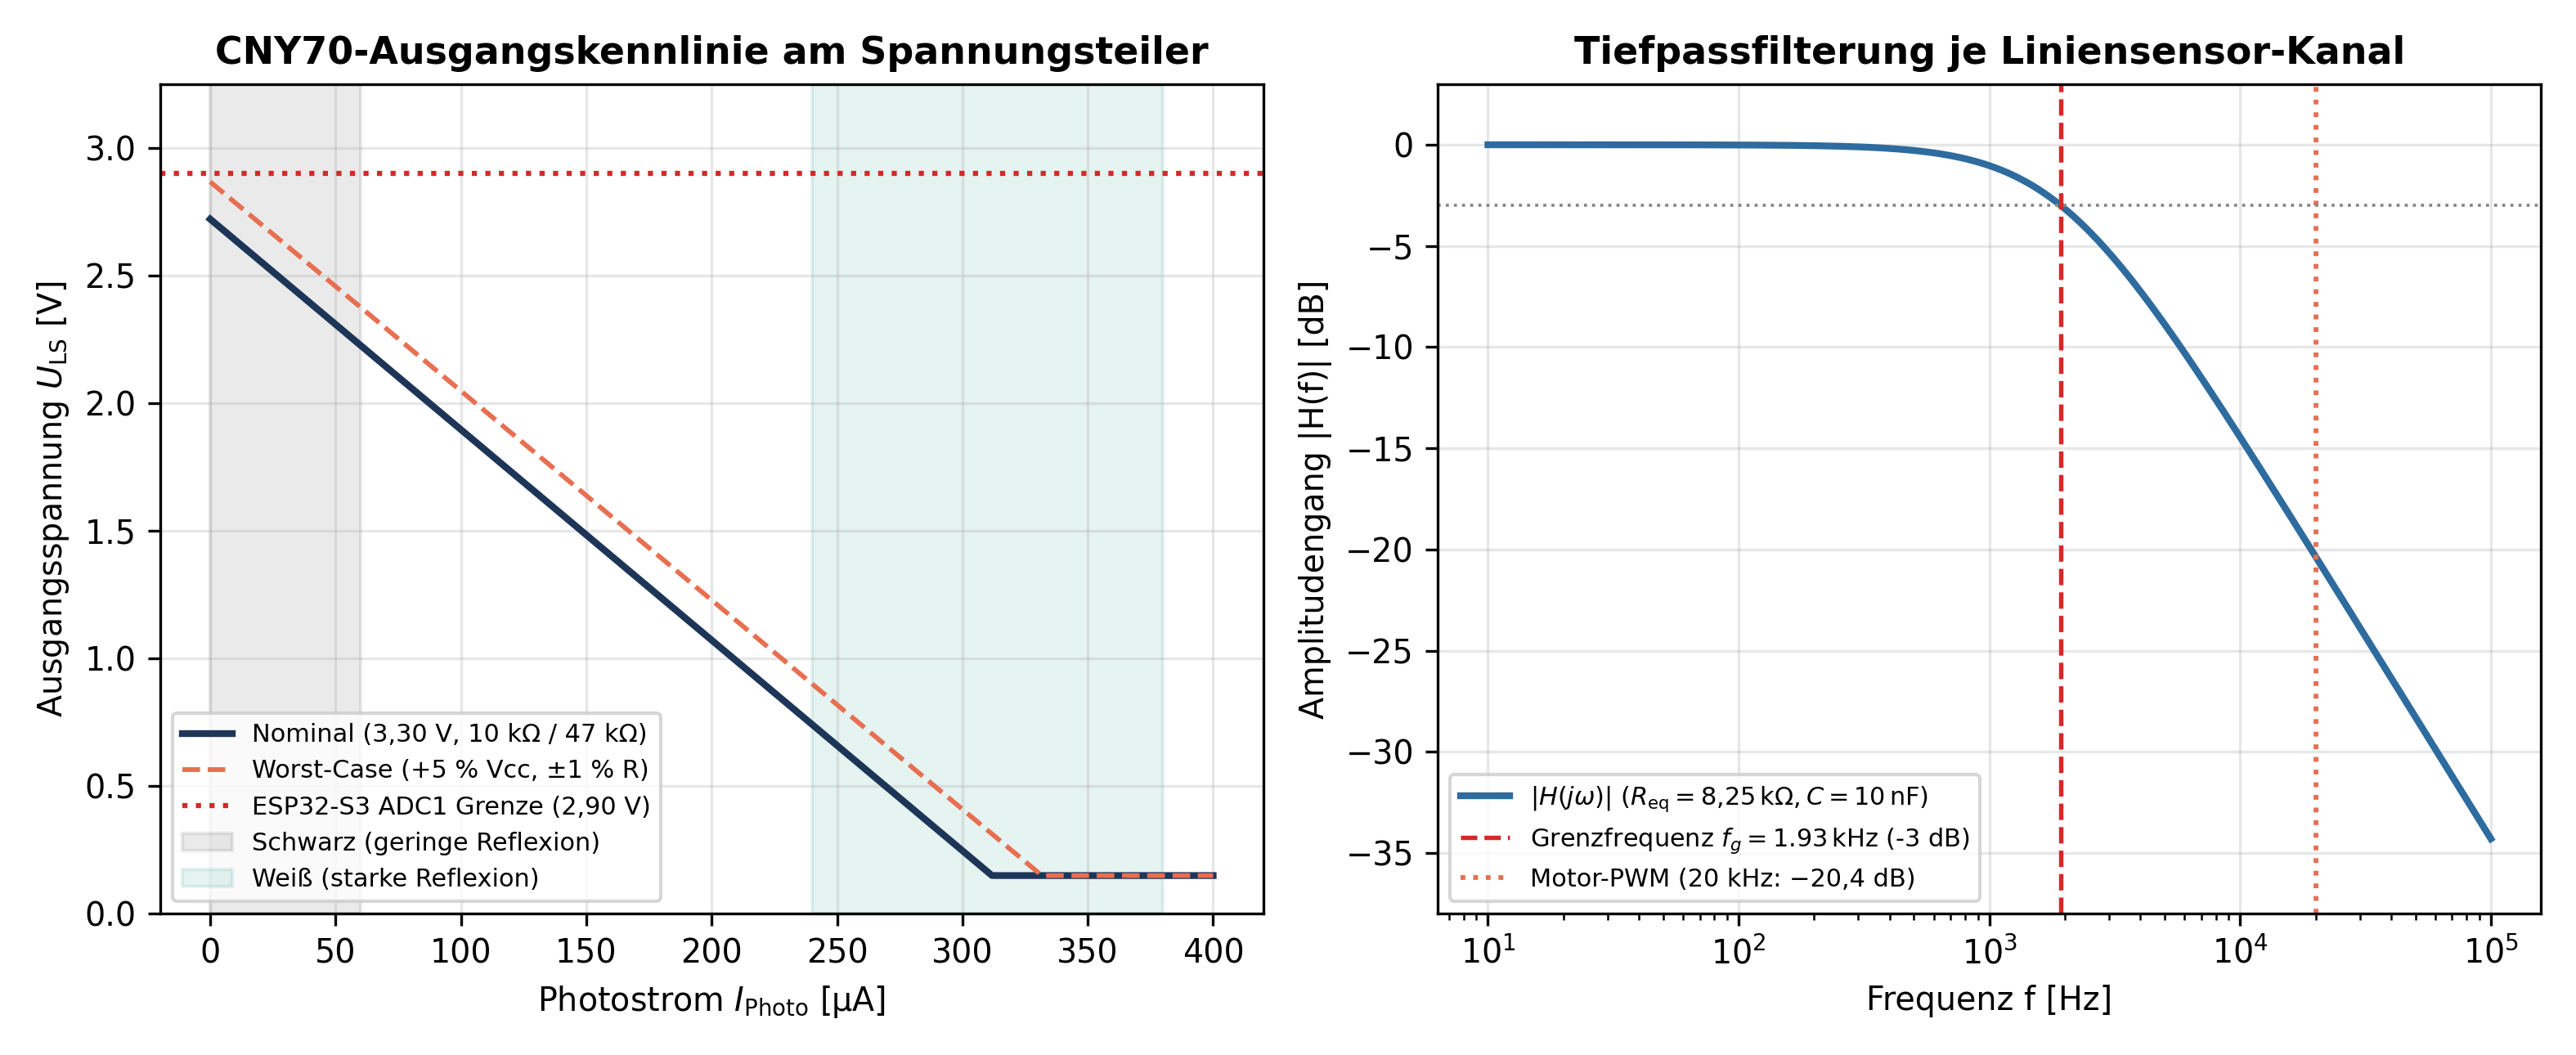
\includegraphics[width=0.98\textwidth]{figures/fig_cny70_transfer_rc.png}
  \caption{Berechnete Ausgangskennlinie $U_{\mathrm{LS}}(I_{\mathrm{Photo}})$ (links) und Tiefpass-Amplitudengang $|H(f)|$ (rechts) der Liniensensor-Platine R2.}
  \label{fig:cny70_transfer}
\end{figure}

\subsection{PCB-Layout, Höhenkette und KiCad-Regelprüfung (ERC/DRC)}
Die Leiterplatte wurde zweilagig in FR4 (\qtyproduct{76 x 32 x 1,6}{\milli\meter}, \qty{35}{\micro\meter} Kupferauflage, vier \qty{3,2}{\milli\meter}-NPTH-Bohrungen im Raster \qtyproduct{68 x 24}{\milli\meter}) geroutet. Sämtliche SMD-Komponenten (0805/1206-Widerstände und -Kondensatoren, SOT-23-Transistoren, seitlicher 10-poliger JST-GH-Steckverbinder \texttt{J2} \cite{JST_GH}) sitzen auf der Oberseite (\texttt{F.Cu}), während die sechs \emph{CNY70}-Sensoren im \qty{10}{\milli\meter}-Raster auf der Unterseite (\texttt{B.Cu}) mit Blickrichtung Fahrbahn bestückt werden. Die Unterseite trägt eine großflächige, geschlossene Massefläche (\texttt{GND}) mit kupferfreien Sperrzonen um die vier M3-Schraubköpfe.

\begin{figure}[htbp]
  \centering
  \begin{subfigure}[b]{0.48\textwidth}
    \centering
    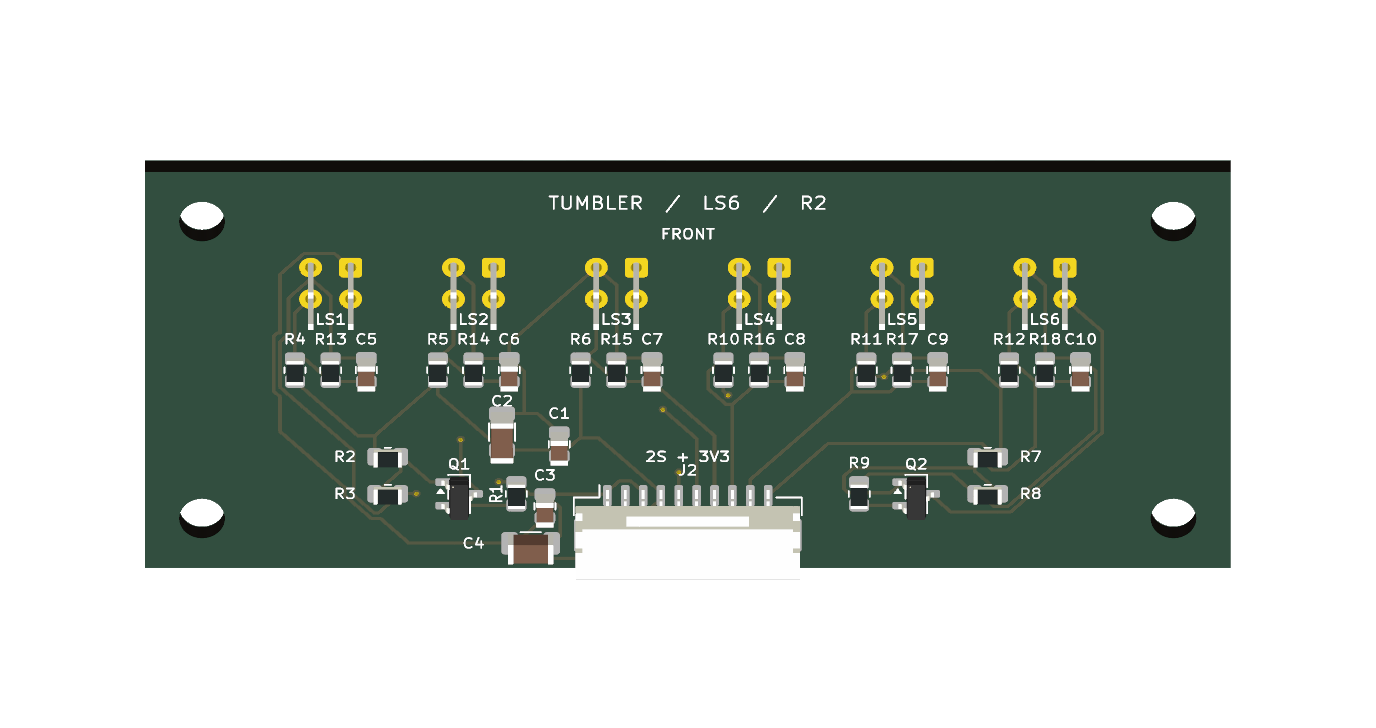
\includegraphics[width=\textwidth]{figures/pcb_ls_oben.png}
    \caption{Oberseite (\texttt{F.Cu}): SMD-Filter, Stromsenken \& JST-GH.}
    \label{fig:pcb_ls_oben}
  \end{subfigure}
  \hfill
  \begin{subfigure}[b]{0.48\textwidth}
    \centering
    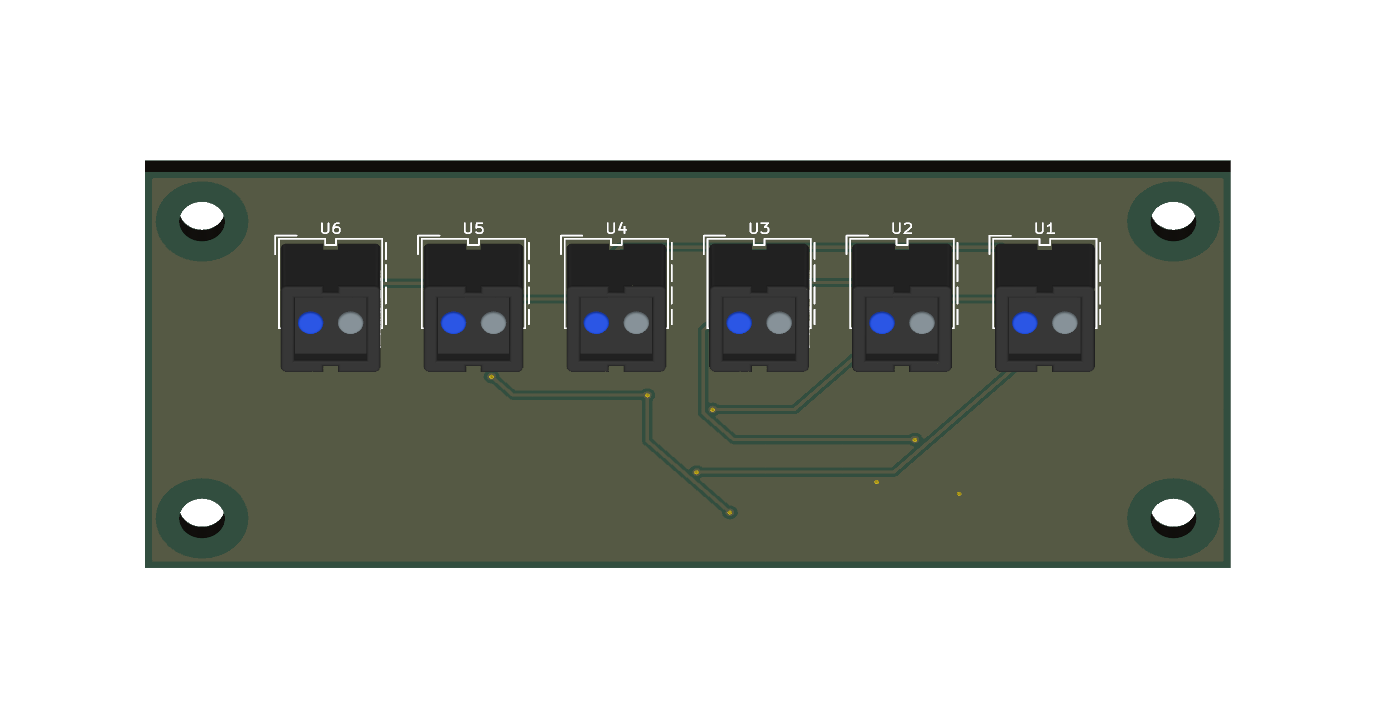
\includegraphics[width=\textwidth]{figures/pcb_ls_unten.png}
    \caption{Unterseite (\texttt{B.Cu}): 6$\times$ CNY70 im \qty{10}{\milli\meter}-Raster.}
    \label{fig:pcb_ls_unten}
  \end{subfigure}
  \caption{3D-CAD-Ansichten der neu gerouteten Liniensensor-Platine R2 (\qtyproduct{76 x 32}{\milli\meter}) aus KiCad.}
  \label{fig:pcb_ls_views}
\end{figure}

Ein praxisnahes Detail ergab sich beim Electrical Rules Check (\gls{erc}): Das offizielle KiCad-Standardsymbol des \emph{CNY70} deklariert den Phototransistor-Emitter (Pin~4) als \texttt{open\_emitter}, was bei direkter Masseanbindung sechs künstliche Pin-Typ-Konflikte mit dem \texttt{PWR\_FLAG} erzeugt. Statt die ERC-Regel blind abzuschalten, wurde eine projektlokale Symbolkopie (\texttt{Tumbler\_Sensor.kicad\_sym}) angelegt, die Pin~4 elektrisch korrekt als passiven Transistoranschluss führt. Die abschließende Prüfung in KiCad~9.0.9 (37 elektrische Bauteile, 19 Netze, \qty{0,25}{\milli\meter} Leiterbahnbreite, \qty{0,20}{\milli\meter} Mindestabstand, \qty{0,60}/\qty{0,30}{\milli\meter} Vias) schloss mit **0 ERC-Fehlern, 0 ERC-Warnungen und 0 DRC-Verletzungen** ab.

Für die mechanische Integration gilt eine definierte Höhenkette: Bei einem optischen Arbeitsabstand von \qty{2,0}{\milli\meter} über der Fahrbahn, \qty{6,0}{\milli\meter} Bauhöhe des CNY70-Gehäuses und \qty{0,5}{\milli\meter} Löt-Sitzabstand liegt die PCB-Unterseite auf \qty{8,5}{\milli\meter} und die Oberseite auf \qty{10,1}{\milli\meter} über Boden. Abbildung~\ref{fig:pcb_ls_halter} zeigt den für erste Vorversuche erstellten Prüfhalter; im finalen Unibody-Chassis~v10.0 wird die Platine direkt von unten gegen den \qty{8,0}{\milli\meter} starken Frontflansch verschraubt.

\begin{figure}[htbp]
  \centering
  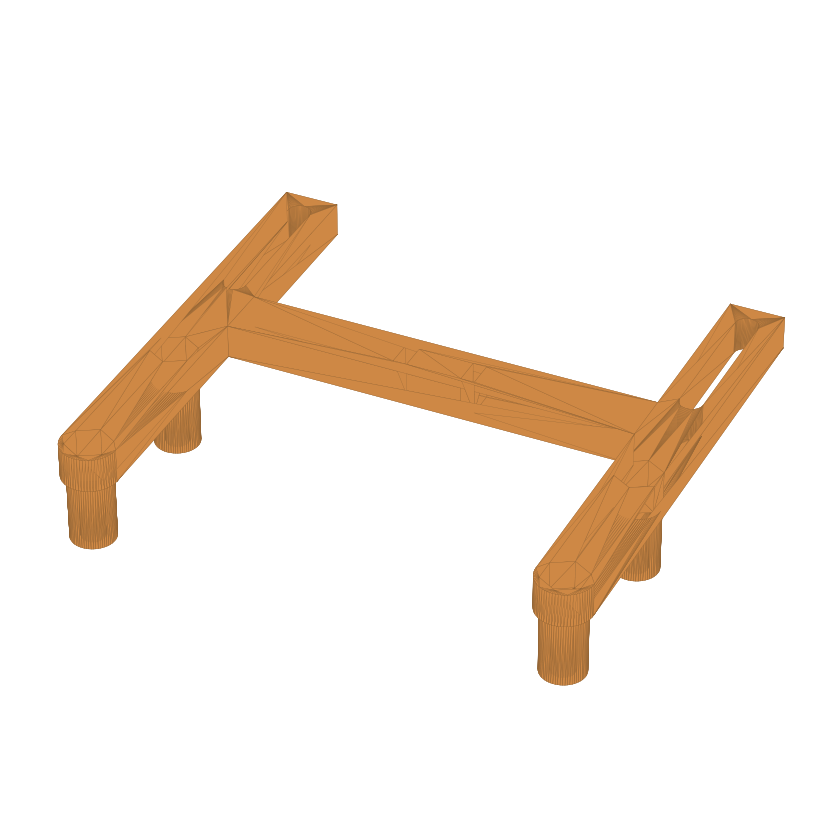
\includegraphics[width=0.58\textwidth]{figures/pcb_ls_halter.png}
  \caption{Mechanische CAD-Ansicht des Prototyp-Sensorhalters für Vorversuche am Liniensensor.}
  \label{fig:pcb_ls_halter}
\end{figure}

% ==============================================================================
\section{Hauptplatine (Tumbler2\_Redesign -- Stufe 1 Signalteil)}
\label{sec:hauptplatine}
% ==============================================================================
Parallel zur Liniensensor-Platine wurde der Schaltplan der Hauptplatine (\texttt{Tumbler2\_Redesign}, \qtyproduct{76,962 x 80,518 x 1,60}{\milli\meter}, M3-Bohrraster \qtyproduct{65,0 x 64,0}{\milli\meter}) in KiCad~10 strukturell bereinigt und auf die neue Sensorik abgestimmt. Der Entwurf wurde bewusst in zwei klar abgegrenzte Ausbaustufen unterteilt: \emph{Stufe~1} (Signalteil, Busgruppen, MCU-Pinzuordnung und geprüfte Netzliste) sowie \emph{Stufe~2} (Leistungspfad, 2S-Ladeschaltung, Verpolschutz und finale Bauteilfestlegung).

\subsection{Wesentliche Änderungen im Signalteil (Stufe 1)}
Gegenüber dem ursprünglichen Arbeitsstand wurden folgende Verbesserungen umgesetzt und durch 51 automatisierte Netzlistenprüfungen (alle 51 \texttt{PASS}) abgesichert:
\begin{itemize}
  \item \textbf{Explizite Busgruppen:} Alle Hierarchie-Übergänge wurden sauber typisiert (\texttt{USB:\{DN DP\}}, \texttt{I2C:\{SDA SCL\}}, \texttt{Motor A:\{AIN1 AIN2 ENCA\_A ENCB\_A\}} und \texttt{Motor B:\{BIN1 BIN2 ENCA\_B ENCB\_B\}}).
  \item \textbf{1:1-Anbindung des Liniensensors (\texttt{J2}):} Ein vertikaler 10-poliger JST-GH-Steckverbinder (\texttt{BM10B-GHS-TBT}) verbindet die sechs Kanäle \texttt{LS1}--\texttt{LS6} über je einen \qty{100}{\ohm}-Serien-Schutzwiderstand (\texttt{R3}, \texttt{R4}, \texttt{R29}--\texttt{R32}, 0603, \qty{0,1}{\watt}) direkt mit sechs Kanälen des \texttt{ADC1} am ESP32-S3 (Tabelle~\ref{tab:j2_pinout}). Die \qty{100}{\ohm}-Widerstände schützen die GPIO-Eingänge vor ESD und kapazitiven Umladespitzen, ohne die \qty{8,25}{\kilo\ohm}-Quellenimpedanz der Sensorplatine nennenswert zu verfälschen.
  \item \textbf{Konfliktfreie Pin-Umschichtung:} Da \texttt{GPIO9} und \texttt{GPIO10} nun für \texttt{LS5} und \texttt{LS6} auf \texttt{ADC1} reserviert sind, wurden der Benutzertaster auf \texttt{GPIO15} und das optionale Echo-Signal auf \texttt{GPIO16} verlegt.
  \item \textbf{USB-C- und LED-Korrektur:} Die USB-Datenleitungen erhielten \qty{22}{\ohm}-Serienwiderstände (\texttt{R33}, \texttt{R34}, 0603) unmittelbar am ESP32-S3 gemäß Espressif-Design-Guideline \cite{EspressifHWGuide}. Bei \texttt{R28} wurde ein fehlerhafter \qty{5}{\volt}-Pull-up gegen einen \qty{10}{\kilo\ohm}-Pulldown nach \texttt{GND} ersetzt.
\end{itemize}

\begin{table}[htbp]
\centering
\caption{1:1-Steckerbelegung von \texttt{J2} (10-pol. JST GH) zwischen Liniensensor und Hauptplatine.}
\label{tab:j2_pinout}
\begin{tabular}{@{}c l c c l@{}}
\toprule
\textbf{Pin J2} & \textbf{Netzname} & \textbf{ESP32-S3 GPIO} & \textbf{ADC-Kanal} & \textbf{Funktion / Hinweis} \\
\midrule
1 & \texttt{GND} & -- & -- & Hauptmasse (Rückleitung) \\
2 & \texttt{VBAT\_SW} & -- & -- & Geschaltete 2S-Akkuspannung (\qtyrange{6,4}{8,4}{\volt}) \\
3 & \texttt{GND} & -- & -- & Zweite Masseleitung (Sensor-Referenz) \\
4 & \texttt{+3.3V} & -- & -- & Geregelte \qty{3,3}{\volt}-Versorgung \\
5 & \texttt{LS1} & \texttt{GPIO4} & \texttt{ADC1\_CH3} & CNY70 \texttt{U1} (links außen), über \qty{100}{\ohm} (\texttt{R3}) \\
6 & \texttt{LS2} & \texttt{GPIO5} & \texttt{ADC1\_CH4} & CNY70 \texttt{U2}, über \qty{100}{\ohm} (\texttt{R4}) \\
7 & \texttt{LS3} & \texttt{GPIO6} & \texttt{ADC1\_CH5} & CNY70 \texttt{U3} (links Mitte), über \qty{100}{\ohm} (\texttt{R29}) \\
8 & \texttt{LS4} & \texttt{GPIO7} & \texttt{ADC1\_CH6} & CNY70 \texttt{U4} (rechts Mitte), über \qty{100}{\ohm} (\texttt{R30}) \\
9 & \texttt{LS5} & \texttt{GPIO9} & \texttt{ADC1\_CH8} & CNY70 \texttt{U5}, über \qty{100}{\ohm} (\texttt{R31}) \\
10 & \texttt{LS6} & \texttt{GPIO10} & \texttt{ADC1\_CH9} & CNY70 \texttt{U6} (rechts außen), über \qty{100}{\ohm} (\texttt{R32}) \\
\bottomrule
\end{tabular}
\end{table}

Abbildung~\ref{fig:pcb_main_sch} zeigt die überarbeiteten Schaltplanseiten des Mikrocontroller- und LED-Teils aus dem KiCad-Projekt \texttt{Tumbler\_Stage1}. Bewusst offen für Stufe~2 (und im Labor vor der Fertigungsfreigabe noch abzuschließen) ist die Durchschaltung von \texttt{VBAT\_SW} an \texttt{J2.2} über den noch zu dimensionierenden 2S-Verpolschutz- und Ladekreis.

\begin{figure}[htbp]
  \centering
  \begin{subfigure}[b]{0.54\textwidth}
    \centering
    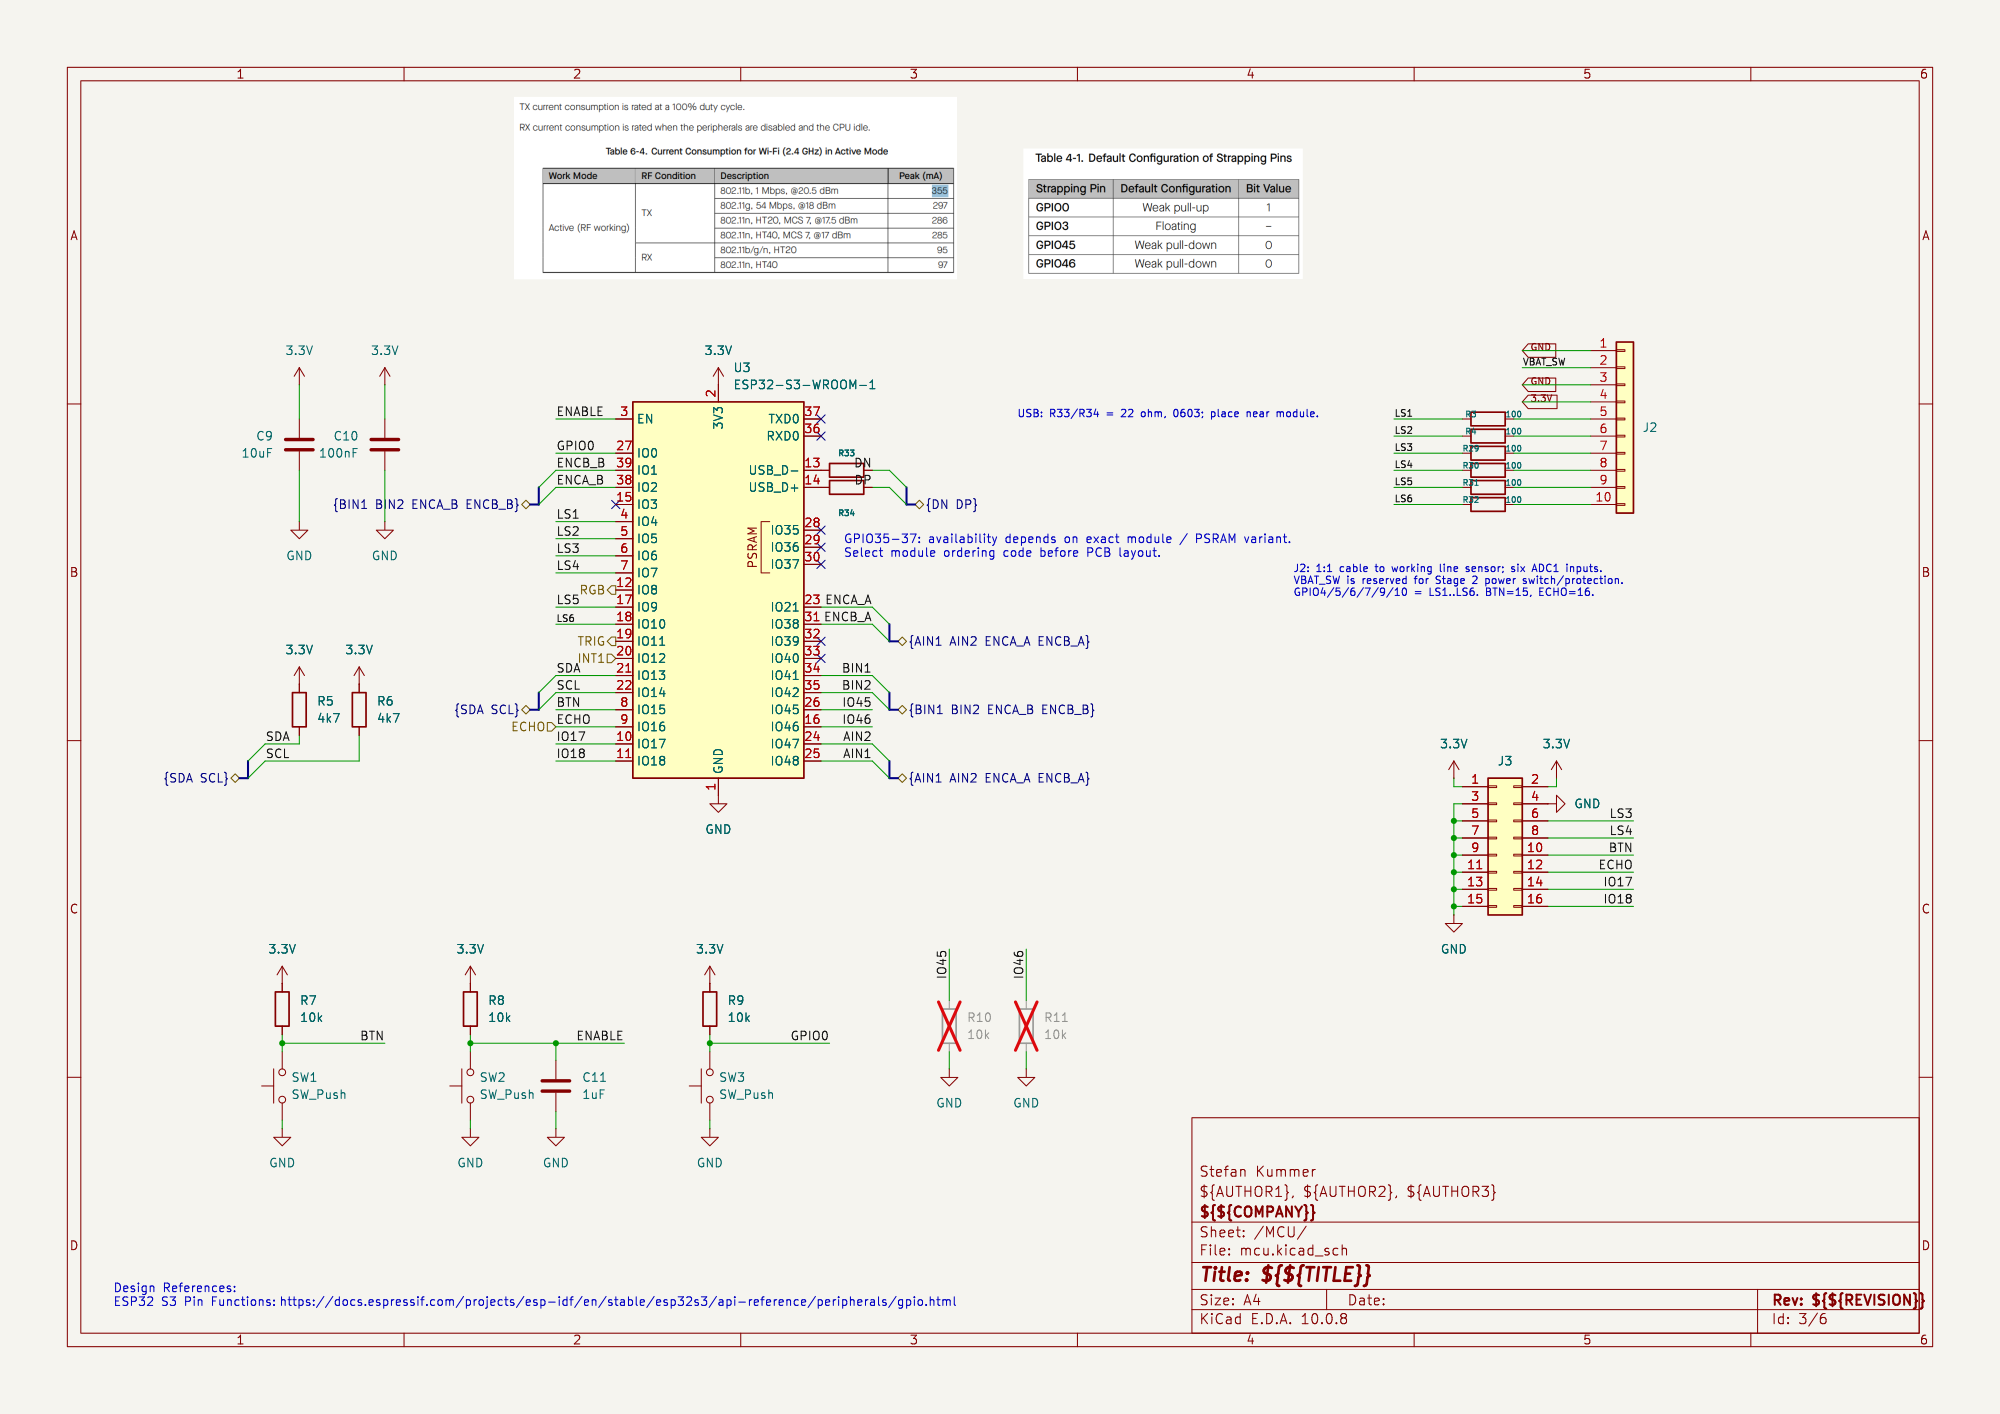
\includegraphics[width=\textwidth]{figures/pcb_main_mcu.png}
    \caption{Mikrocontroller-Schaltplan (\texttt{ESP32-S3}, Busgruppen).}
    \label{fig:pcb_main_mcu}
  \end{subfigure}
  \hfill
  \begin{subfigure}[b]{0.43\textwidth}
    \centering
    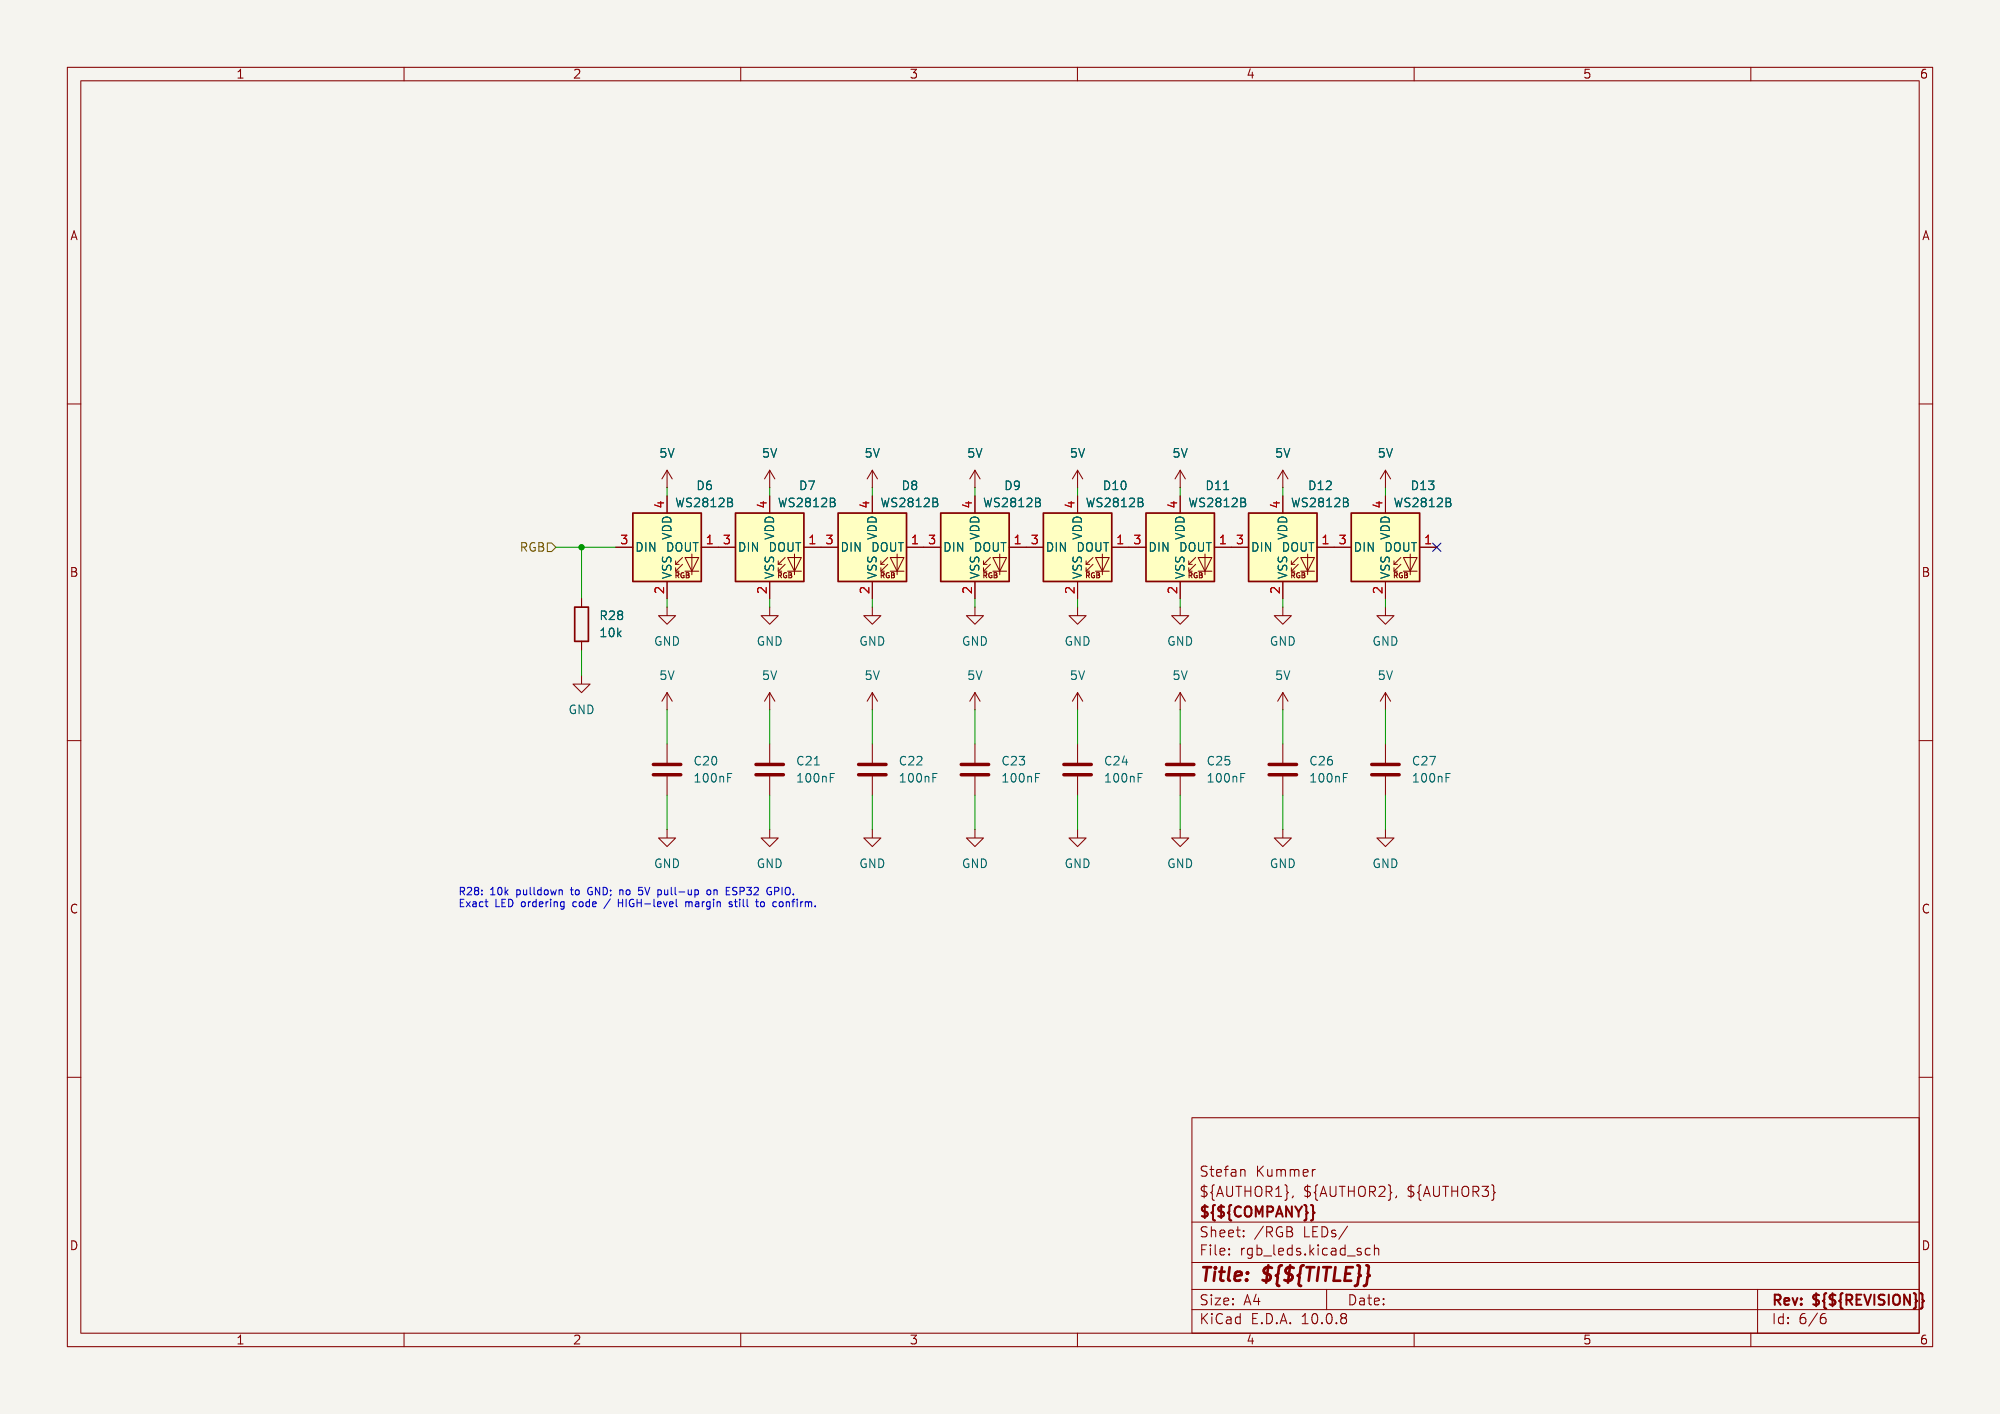
\includegraphics[width=\textwidth]{figures/pcb_main_rgb.png}
    \caption{Status-LED-Teilschaltung (\texttt{R28} Pulldown).}
    \label{fig:pcb_main_rgb}
  \end{subfigure}
  \caption{Schaltplanauszüge der Hauptplatine \texttt{Tumbler\_Stage1} (KiCad~10).}
  \label{fig:pcb_main_sch}
\end{figure}

\subsection{Übergang zu Stufe 2 und Leistungs- bzw. Akkulaufzeitbilanz}
\label{sec:leistungsbilanz}
Die gezielte Netzlistenprüfung von \texttt{Tumbler\_Stage1} bestätigte 51 von 51 Signalverbindungen ohne Befund (ERC-Kategorien \texttt{net\_not\_bus\_member}, \texttt{pin\_not\_driven} und \texttt{multiple\_net\_names} jeweils~0). Im ungefilterten Gesamt-ERC verblieben lediglich drei dokumentierte Meldungen (\texttt{power\_pin\_not\_driven}, \texttt{isolated\_pin\_label} sowie \texttt{pin\_to\_pin}), die direkt auf den bewusst noch offenen Leistungspfad von \texttt{VBAT\_SW} zurückgehen. Dieser wird in Stufe~2 gemeinsam mit der 2S-USB-C-Lade- und Schutzschaltung sowie der endgültigen Entscheidung zwischen \emph{LSM6DSV} und \emph{MPU6050} geschlossen.

Für die Auslegung der Strompfade und Sicherungen wurde eine vollständige Leistungsbilanz bei Nennspannung $U_{\mathrm{Bat}} = \qty{7,4}{\volt}$ aufgestellt (Tabelle~\ref{tab:leistungsbilanz}).

\begin{table}[htbp]
\centering
\caption{Strom- und Leistungsbilanz des Tumbler~v3.0 im normalen Fahrbetrieb und im Blockierfall.}
\label{tab:leistungsbilanz}
\begin{tabular}{@{}p{4.6cm}c c c c@{}}
\toprule
\textbf{Verbraucher} & \textbf{Schiene} & \textbf{Typ. Strom} & \textbf{Max. Strom} & \textbf{Typ. Leistung} \\
\midrule
ESP32-S3-WROOM-1 (Dual-Core) & \qty{3,3}{\volt} & \qty{140}{\milli\ampere} & \qty{350}{\milli\ampere} & \qty{0,46}{\watt} \\
8$\times$ VL53L0/1XV2 (kontinuierlich) & \qty{3,3}{\volt} & \qty{160}{\milli\ampere} & \qty{240}{\milli\ampere} & \qty{0,53}{\watt} \\
6$\times$ CNY70 Phototransistoren + IMU & \qty{3,3}{\volt} & \qty{15}{\milli\ampere} & \qty{25}{\milli\ampere} & \qty{0,05}{\watt} \\
6$\times$ CNY70 IR-LEDs (2 Stränge) & \texttt{VBAT\_SW} & \qty{40}{\milli\ampere} & \qty{52}{\milli\ampere} & \qty{0,30}{\watt} \\
2$\times$ GA37-520 Motoren (Fahrt / Stall) & \texttt{VBAT\_SW} & \qty{600}{\milli\ampere} & \qty{3200}{\milli\ampere} & \qty{4,44}{\watt} \\
\midrule
\textbf{Gesamt (inkl. $\eta_{\mathrm{Buck}} = 90\,\%$)} & \textbf{2S Li-Ion} & \textbf{$\approx \qty{800}{\milli\ampere}$} & \textbf{$\approx \qty{3550}{\milli\ampere}$} & \textbf{$\approx \qty{5,9}{\watt}$} \\
\bottomrule
\end{tabular}
\end{table}

Mit einem gängigen 2S-Li-Ion-Pack der Kapazität $C_{\mathrm{Bat}} = \qty{2600}{\milli\ampere\hour}$ und einer nutzbaren Entladetiefe von \qty{85}{\percent} ergibt sich im kontinuierlichen Fahr- und Einparkbetrieb eine rechnerische Betriebsdauer von:
\begin{equation}
  t_{\mathrm{Betrieb}} \approx \frac{0{,}85 \cdot \qty{2600}{\milli\ampere\hour}}{\qty{800}{\milli\ampere}} \approx \qty{2,76}{\hour}
  \label{eq:akkulaufzeit}
\end{equation}
Damit ist ein ganzer Labor- oder Prüfungstag problemlos mit einer einzigen Akkuladung abdeckbar.

% ==============================================================================
\section{Mechanische Konstruktion und CAD-Evolution (v1 bis v10.0)}
\label{sec:cad_evolution}
% ==============================================================================
Das Fahrgestell bildet das mechanische Rückgrat des Roboters. Statt einer manuellen, schwer änderbaren Maus-Konstruktion wurde das komplette Chassis samt einem 127-Körper-Digital-Mock-Up (\gls{dmu}) parametrisch in Python (\texttt{build123d} / OpenCASCADE BRep-Kern sowie Fusion-360-API-Skripte) nach dem \gls{ssot}-Prinzip aufgebaut. Jede Änderung an Platinenmaßen, Schraubenabständen oder Wandstärken propagiert dadurch automatisch und widerspruchsfrei in das gesamte 3D-Modell.

\subsection{Chronologische Fehleranalyse und Iterationsstufen}
Die Entwicklung durchlief zehn konstruktive Hauptrevisionen, in denen reale Probleme aus der Vorversion schrittweise aufgedeckt und systematisch beseitigt wurden (Tabelle~\ref{tab:cad_evolution}).

\begin{table}[htbp]
\centering
\caption{Entwicklungshistorie des 3D-Chassis von der Nachkonstruktion (v1) bis zum druckfertigen Release (v10.0).}
\label{tab:cad_evolution}
\begin{tabular}{@{}p{1.5cm}p{3.6cm}p{8.9cm}@{}}
\toprule
\textbf{Version} & \textbf{Schwerpunkt} & \textbf{Erkannte Schwachstelle und konstruktive Lösung} \\
\midrule
v1--v2 & Reverse Engineering & Nachbildung des handvermessenen Originalgehäuses (\qtyproduct{120 x 176}{\milli\meter}). Ergebnis: zu wenig Bauraum für 2S-Akku und keine geschützten LiDAR-Aufnahmen. \\
v3 & Integration 6$\times$ LiDAR & Erste integrierte Sensor-Pods für \emph{VL53L0/1XV2} (\qty{19,5}{\milli\meter} Lochabstand). Schwachstelle: zu wenig Platz hinter verlöteten Stiftleisten zum Einstecken von Dupont-Kabeln. \\
v4--v6 & Crash-Bumper \& Stecker-Dummies & Einführung eines \qty{6,0}{\milli\meter} Crash-Bumpers, \qty{4,0}{\milli\meter} Bodenplatte und realer \qty{24}{\milli\meter} roter Stecker-Dummies. Erste automatisierte BRep-Kollisionsprüfung. \\
v7--v8 & Upgrade auf 8$\times$ LiDAR & Erweiterung auf \qty{360}{\degree}-Abdeckung (zusätzliche Front- und Heck-Mittensensoren \texttt{3a}/\texttt{3h}). Akkufach auf \qtyproduct{78,0 x 43,3 x 21,5}{\milli\meter} erweitert. \\
v9 & Zero-Collision-DMU & Beseitigung aller `.solids()[0]`-Trunkierungen (121 Einzelkörper geprüft), Schutz der 4 Standoffs (\texttt{H1}--\texttt{H4}) und geschlossene \qtyrange{3,85}{4,30}{\milli\meter} Pod-Dächer. \\
\textbf{v10.0} & \textbf{Print-Ready DfAM} & \textbf{1)} Blockierende Querwand hinter Motoren ($Y = +2{,}5..+4{,}5\text{ mm}$) komplett entfernt; \textbf{2)} nach oben offener \emph{Slide-In} Schalter-C-Kanal + Snap-On Clip; \textbf{3)} Stadium-Laschentaschen \& \qty{1,80}{\milli\meter} M2-Teardrop-Sacklöcher; \textbf{4)} 4$\times$ M3-Sechskant-Mutterntaschen; \textbf{5)} 100\,\% Watertight STL. \\
\bottomrule
\end{tabular}
\end{table}

Abbildung~\ref{fig:cad_evolution_imgs} illustriert diesen schrittweisen Reifeprozess vom schlichten Ausgangsmodell~(v2) über die erste LiDAR-Integration~(v3) bis zum vollständigen 127-Körper-DMU der Revision~v10.0.

\begin{figure}[htbp]
  \centering
  \begin{subfigure}[b]{0.48\textwidth}
    \centering
    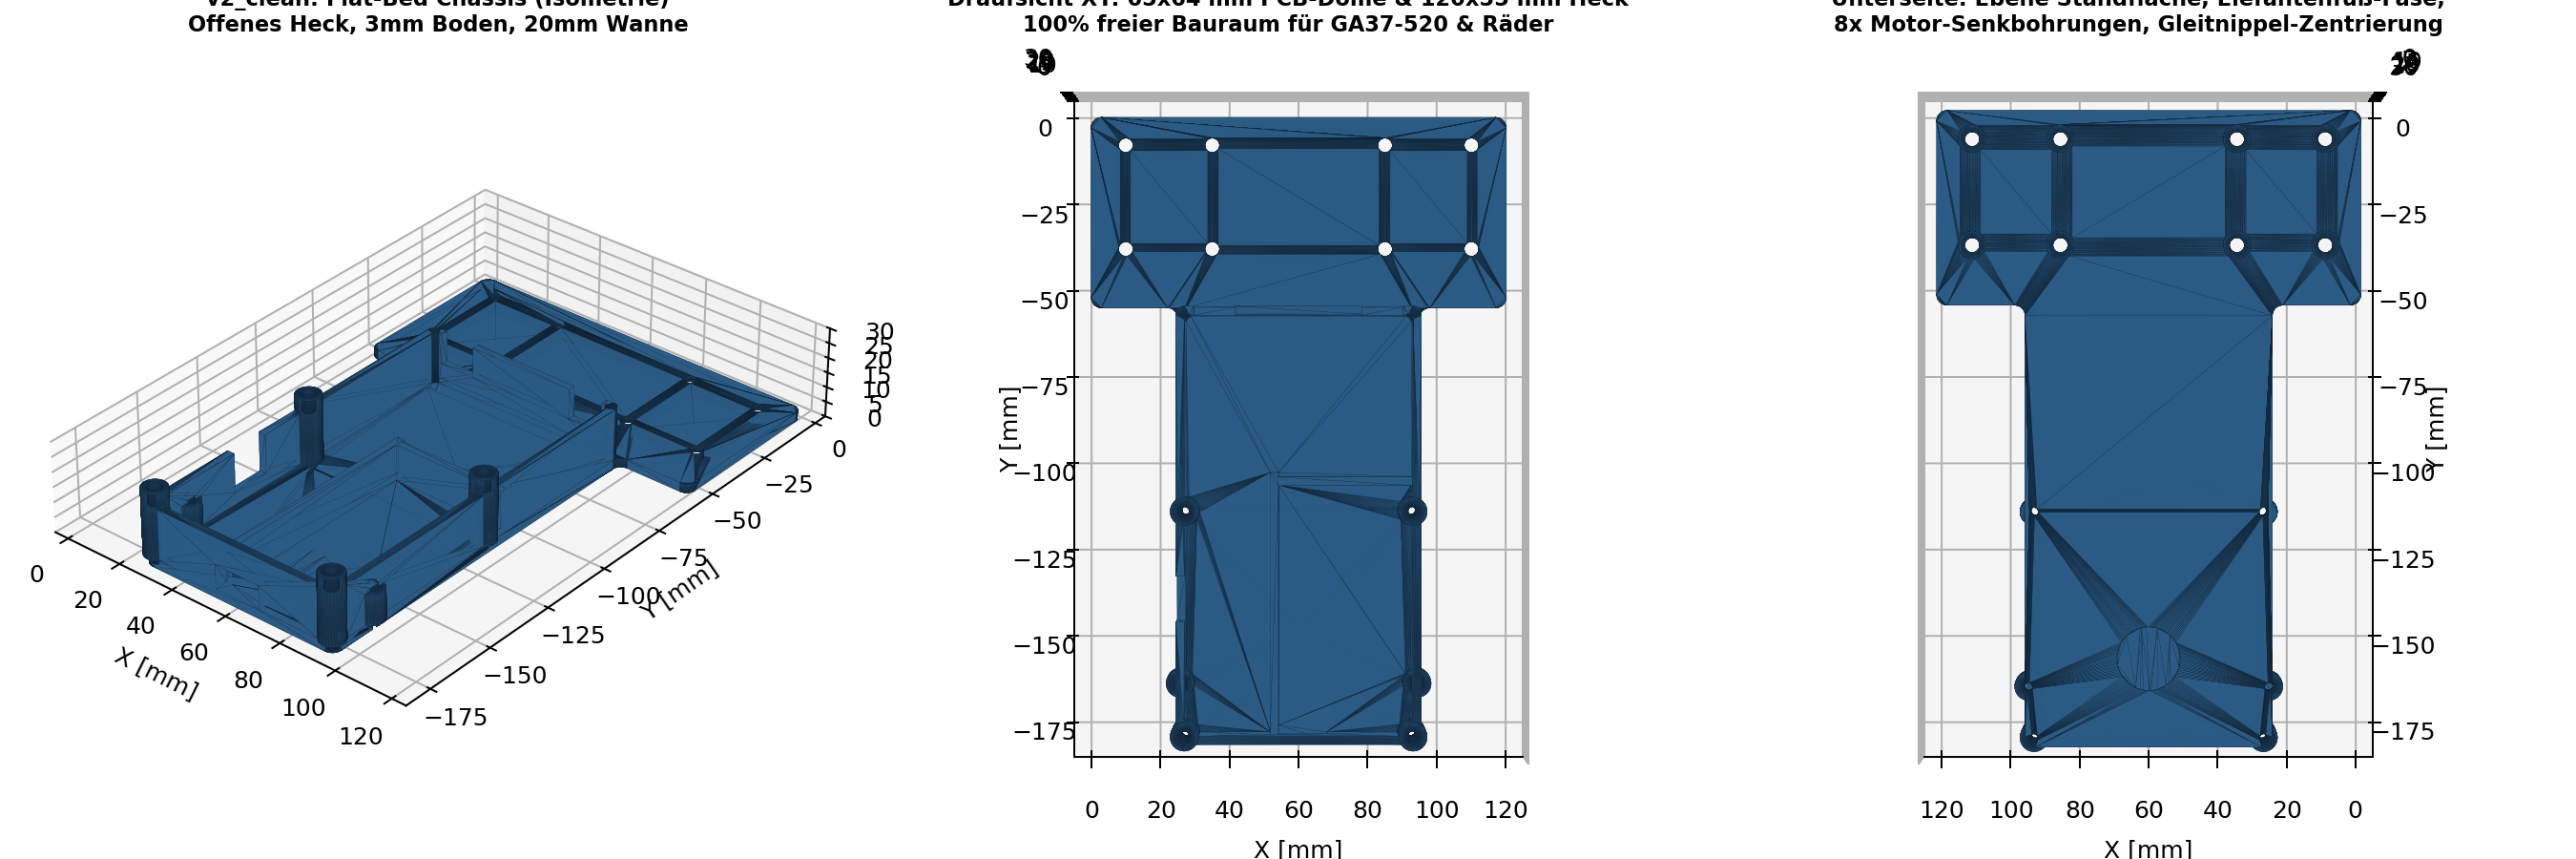
\includegraphics[width=\textwidth]{figures/v2_clean_engineering_views.png}
    \caption{Revision~v2: Nachkonstruktion des Ausgangsgehäuses.}
    \label{fig:cad_v2}
  \end{subfigure}
  \hfill
  \begin{subfigure}[b]{0.48\textwidth}
    \centering
    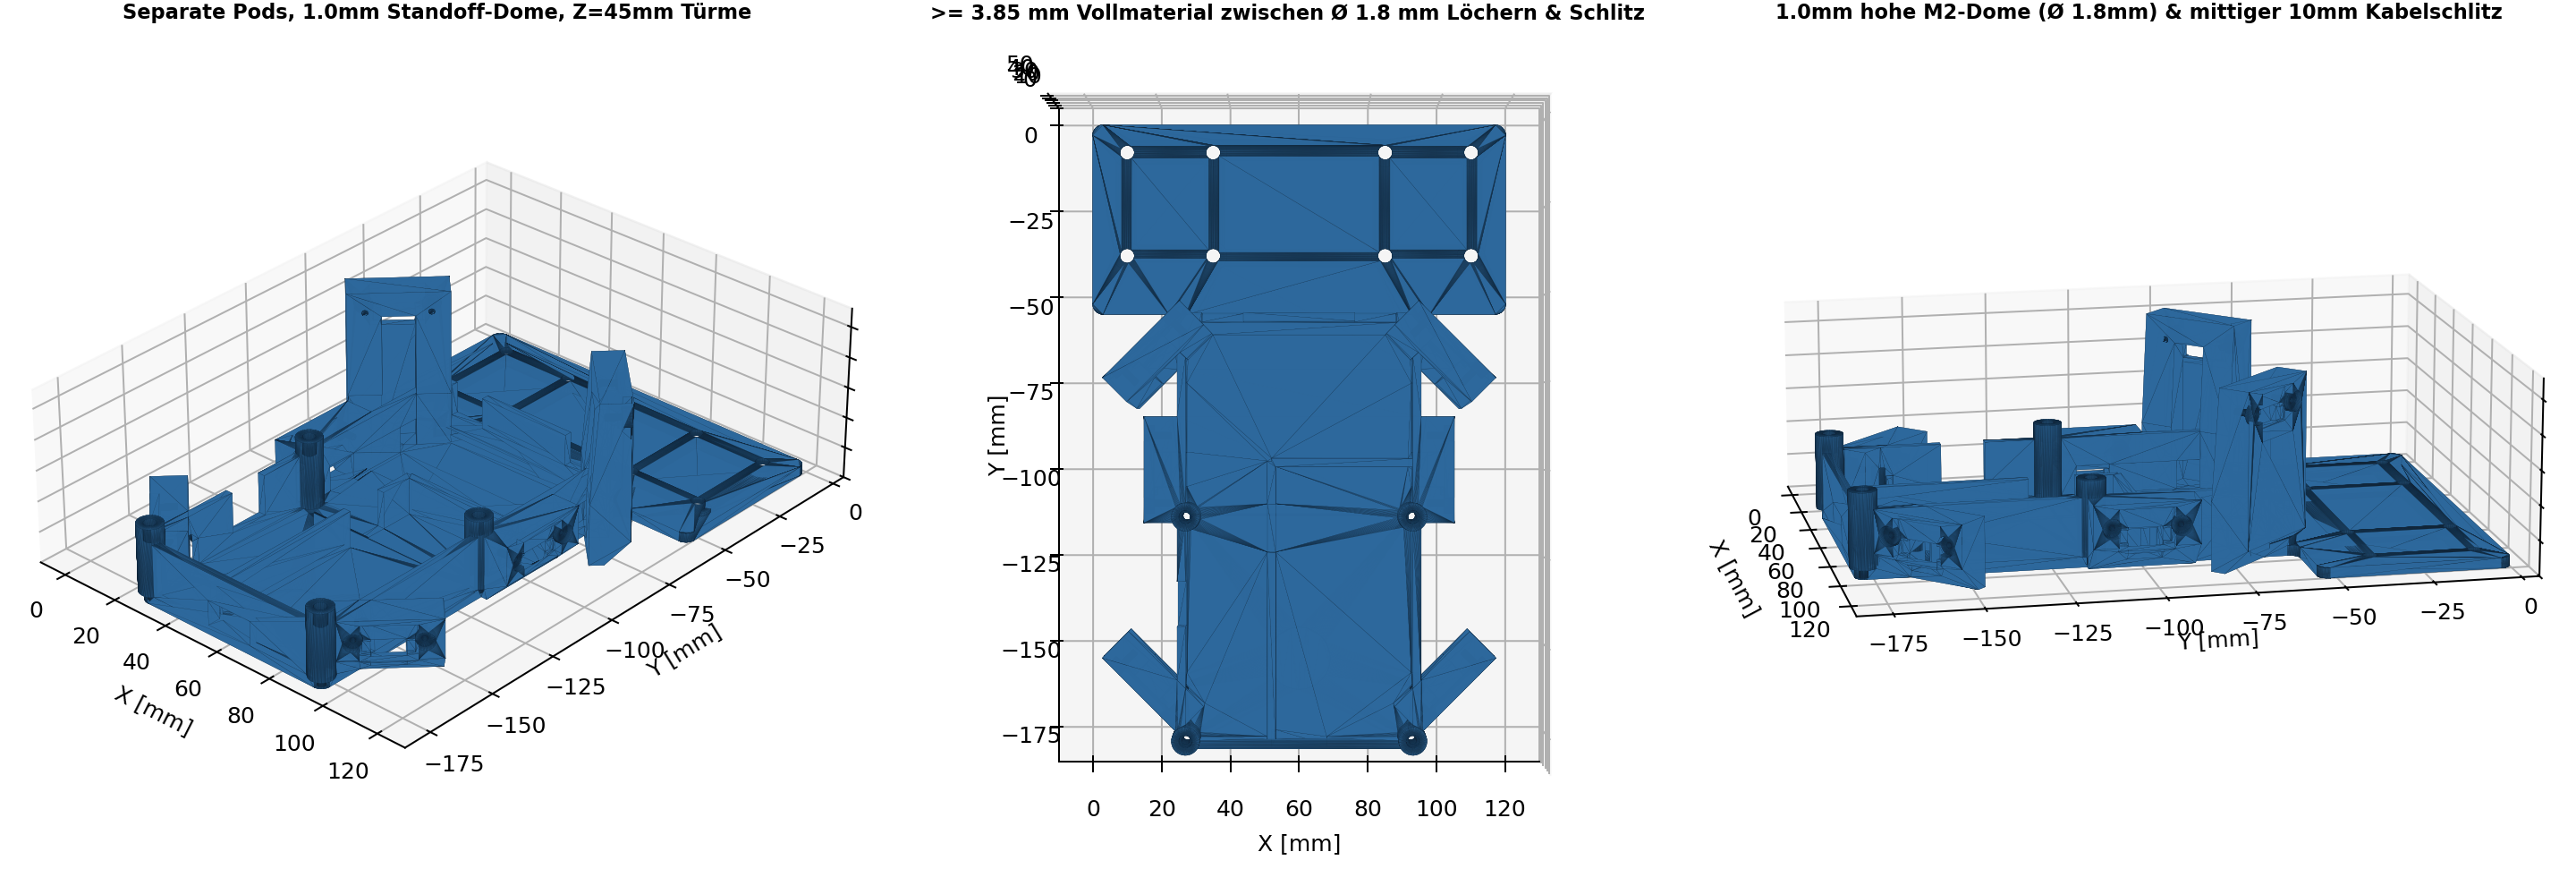
\includegraphics[width=\textwidth]{figures/v3_LiDar_V2_engineering_views.png}
    \caption{Revision~v3: Erste 6-fach-LiDAR-Integration mit Türmen.}
    \label{fig:cad_v3}
  \end{subfigure}
  \vspace{0.4cm}
  \begin{subfigure}[b]{0.98\textwidth}
    \centering
    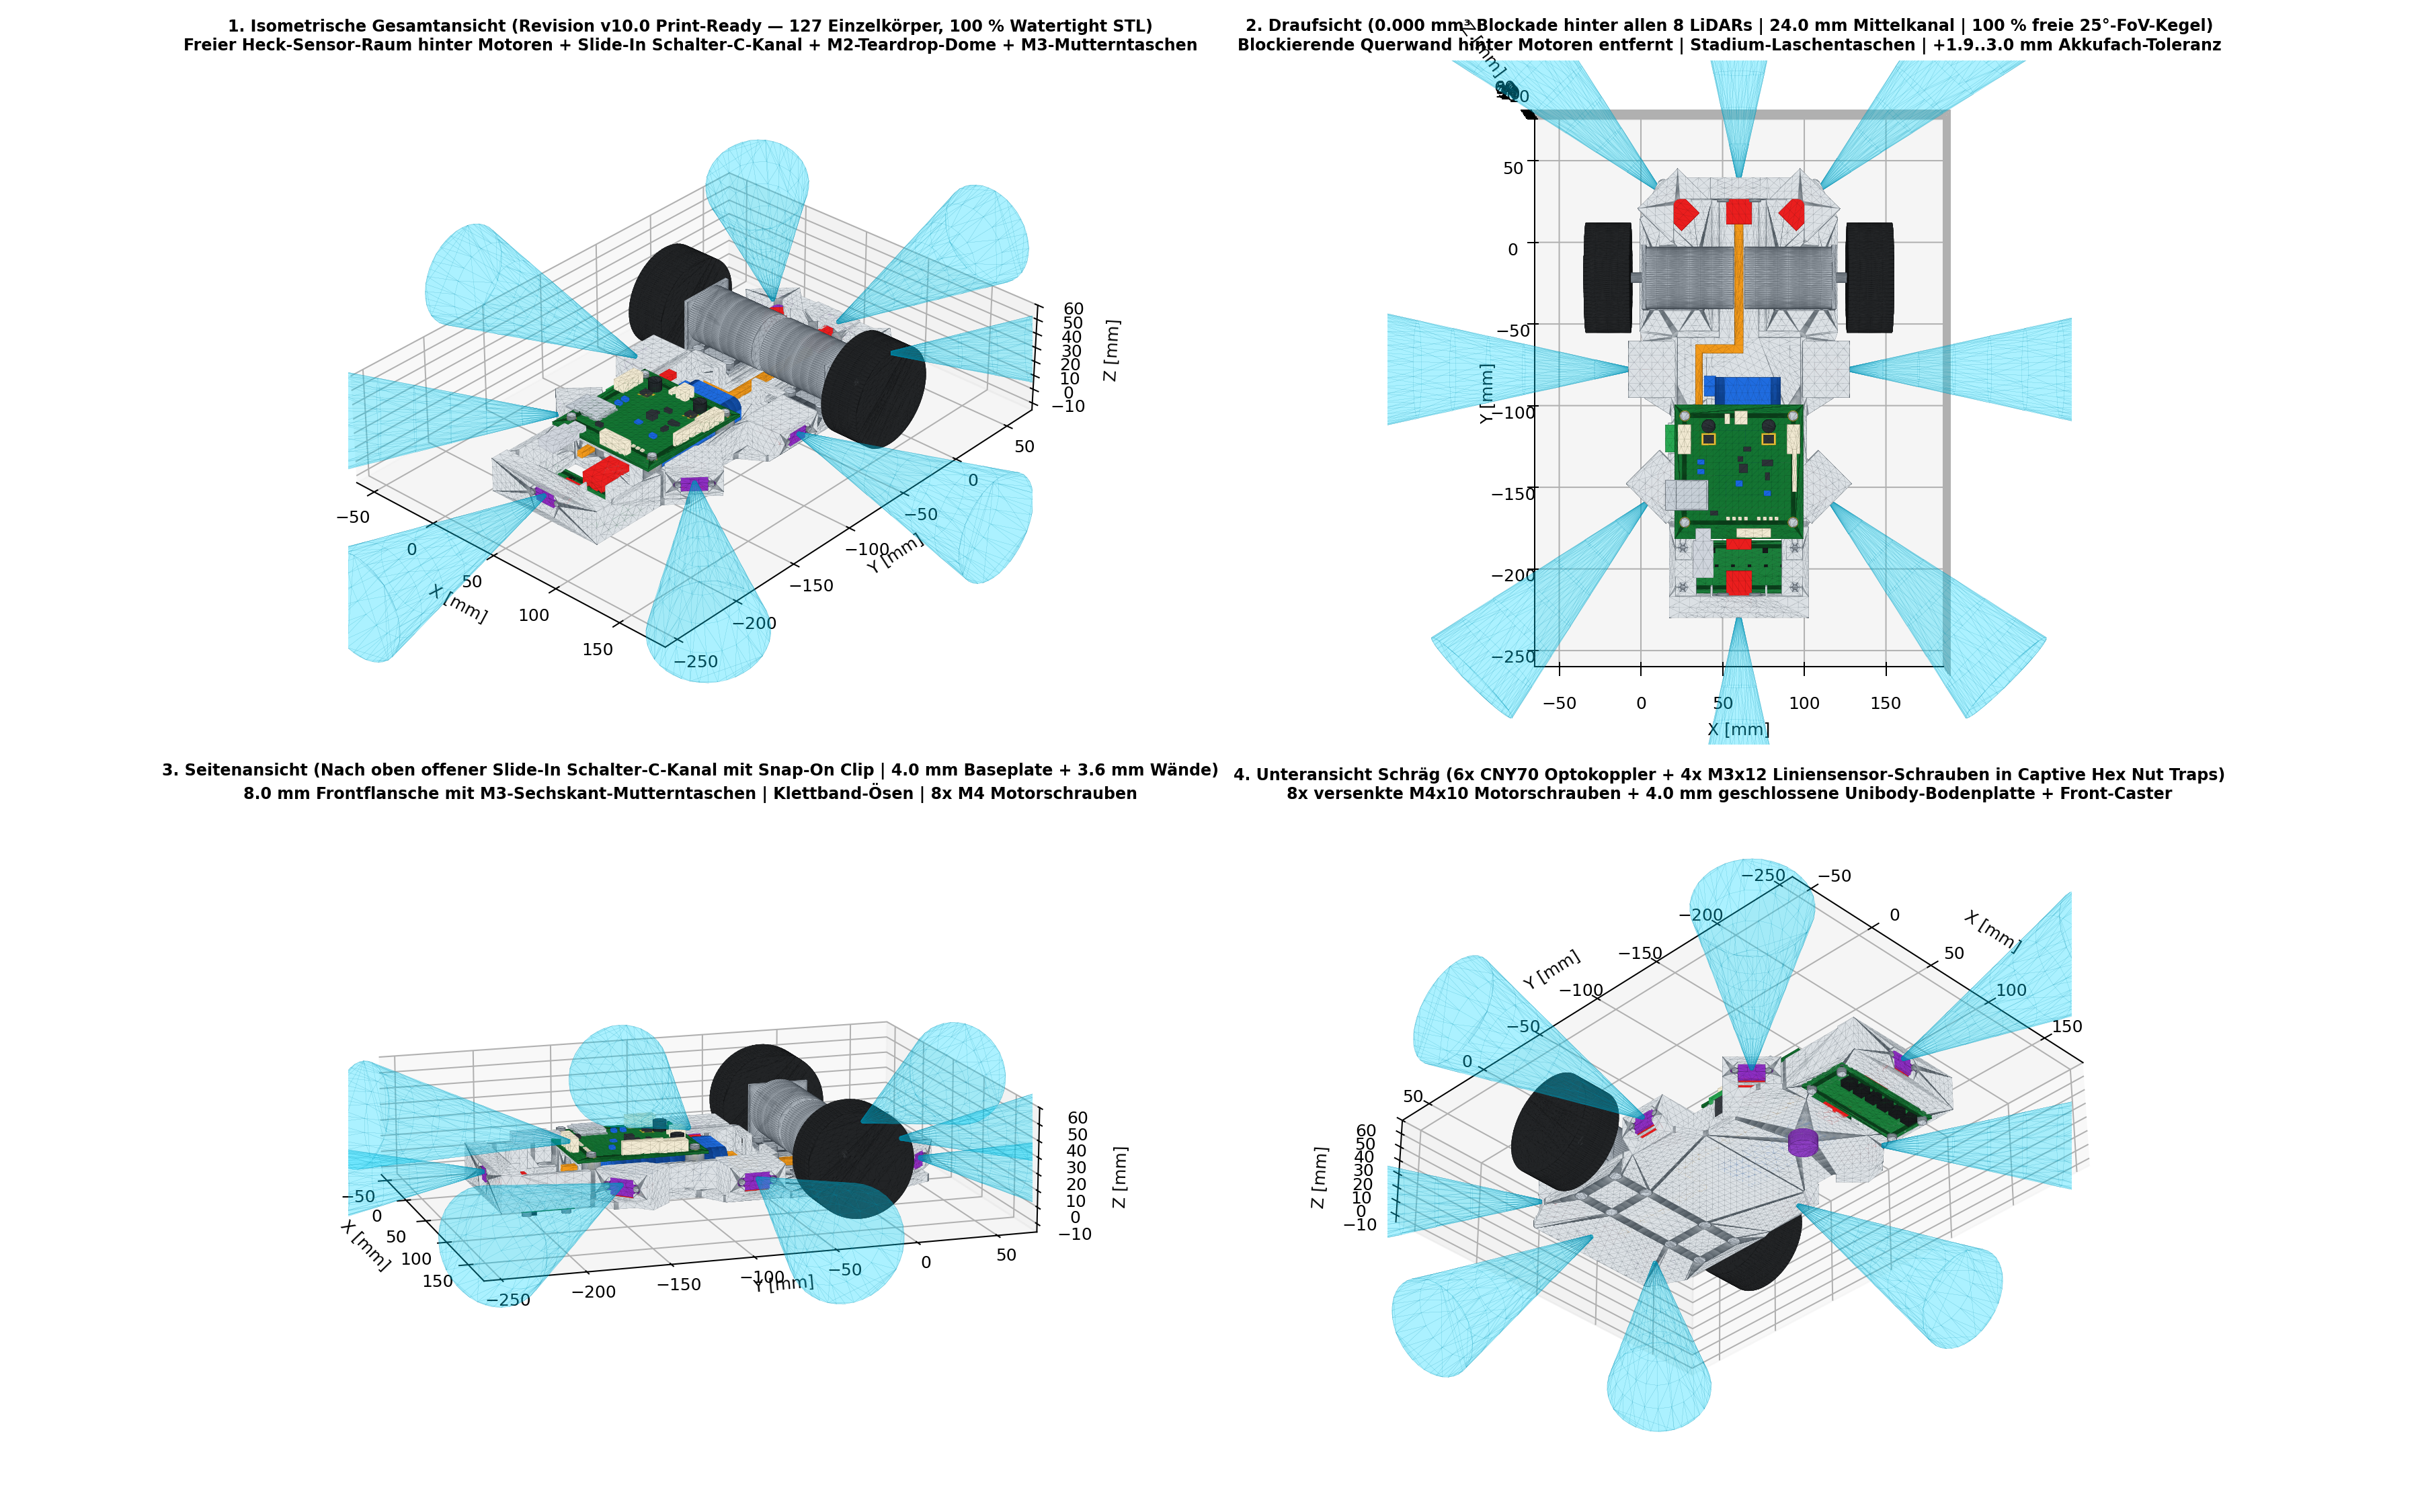
\includegraphics[width=\textwidth]{figures/cad_v10_master_dmu.png}
    \caption{Revision~v10.0 (Print-Ready): Vollständiges 127-Körper-DMU mit 8$\times$ \qty{25}{\degree}-FoV-Sichtkegeln, allen SMD-Bauteilen, 24-mm-Stecker-Dummies, Schrauben und 3D-Kabelbaum (\qty{0,000}{\milli\meter\cubed} Kollision).}
    \label{fig:cad_v10_master}
  \end{subfigure}
  \caption{Evolution des 3D-Chassis vom Grundkörper~(v2) bis zum fertigungsreifen Digital Mock-Up~(v10.0).}
  \label{fig:cad_evolution_imgs}
\end{figure}

\begin{figure}[htbp]
  \centering
  \begin{subfigure}[b]{0.48\textwidth}
    \centering
    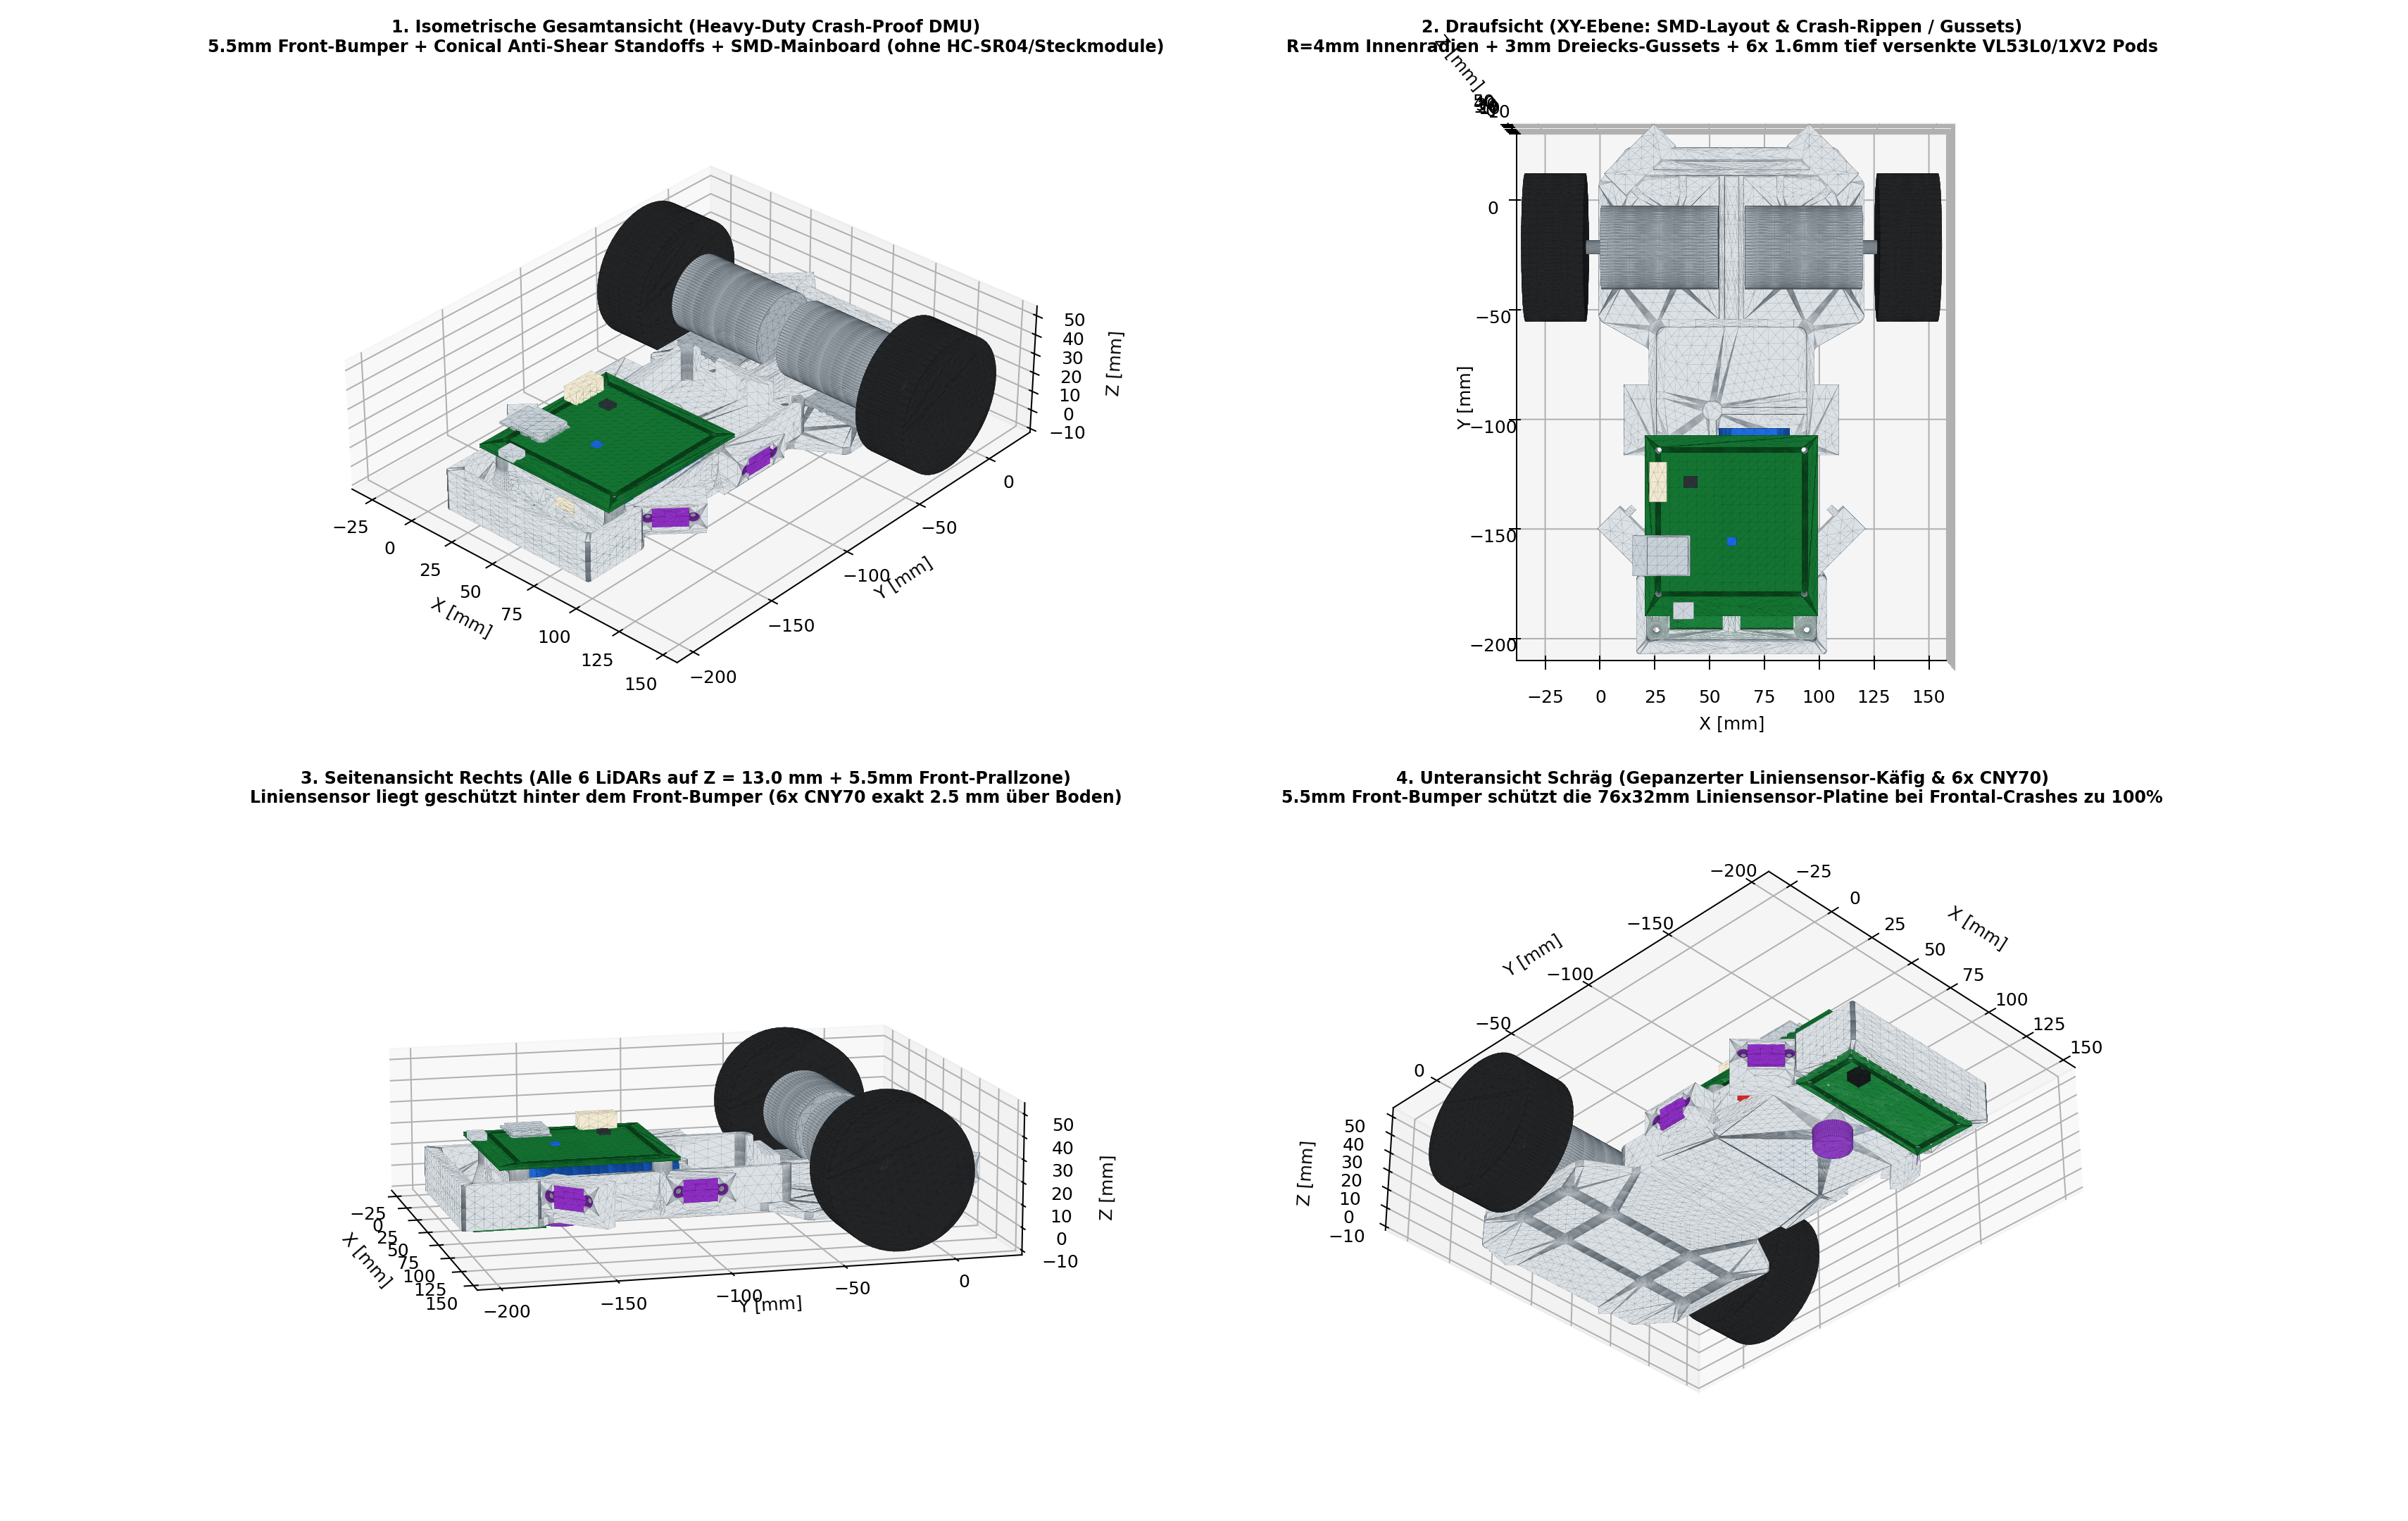
\includegraphics[width=\textwidth]{figures/cad_v4_crashproof.png}
    \caption{Revision~v4: Einführung des 6-mm-Crash-Bumpers und roter 24-mm-Stecker-Dummies.}
    \label{fig:cad_v4}
  \end{subfigure}
  \hfill
  \begin{subfigure}[b]{0.48\textwidth}
    \centering
    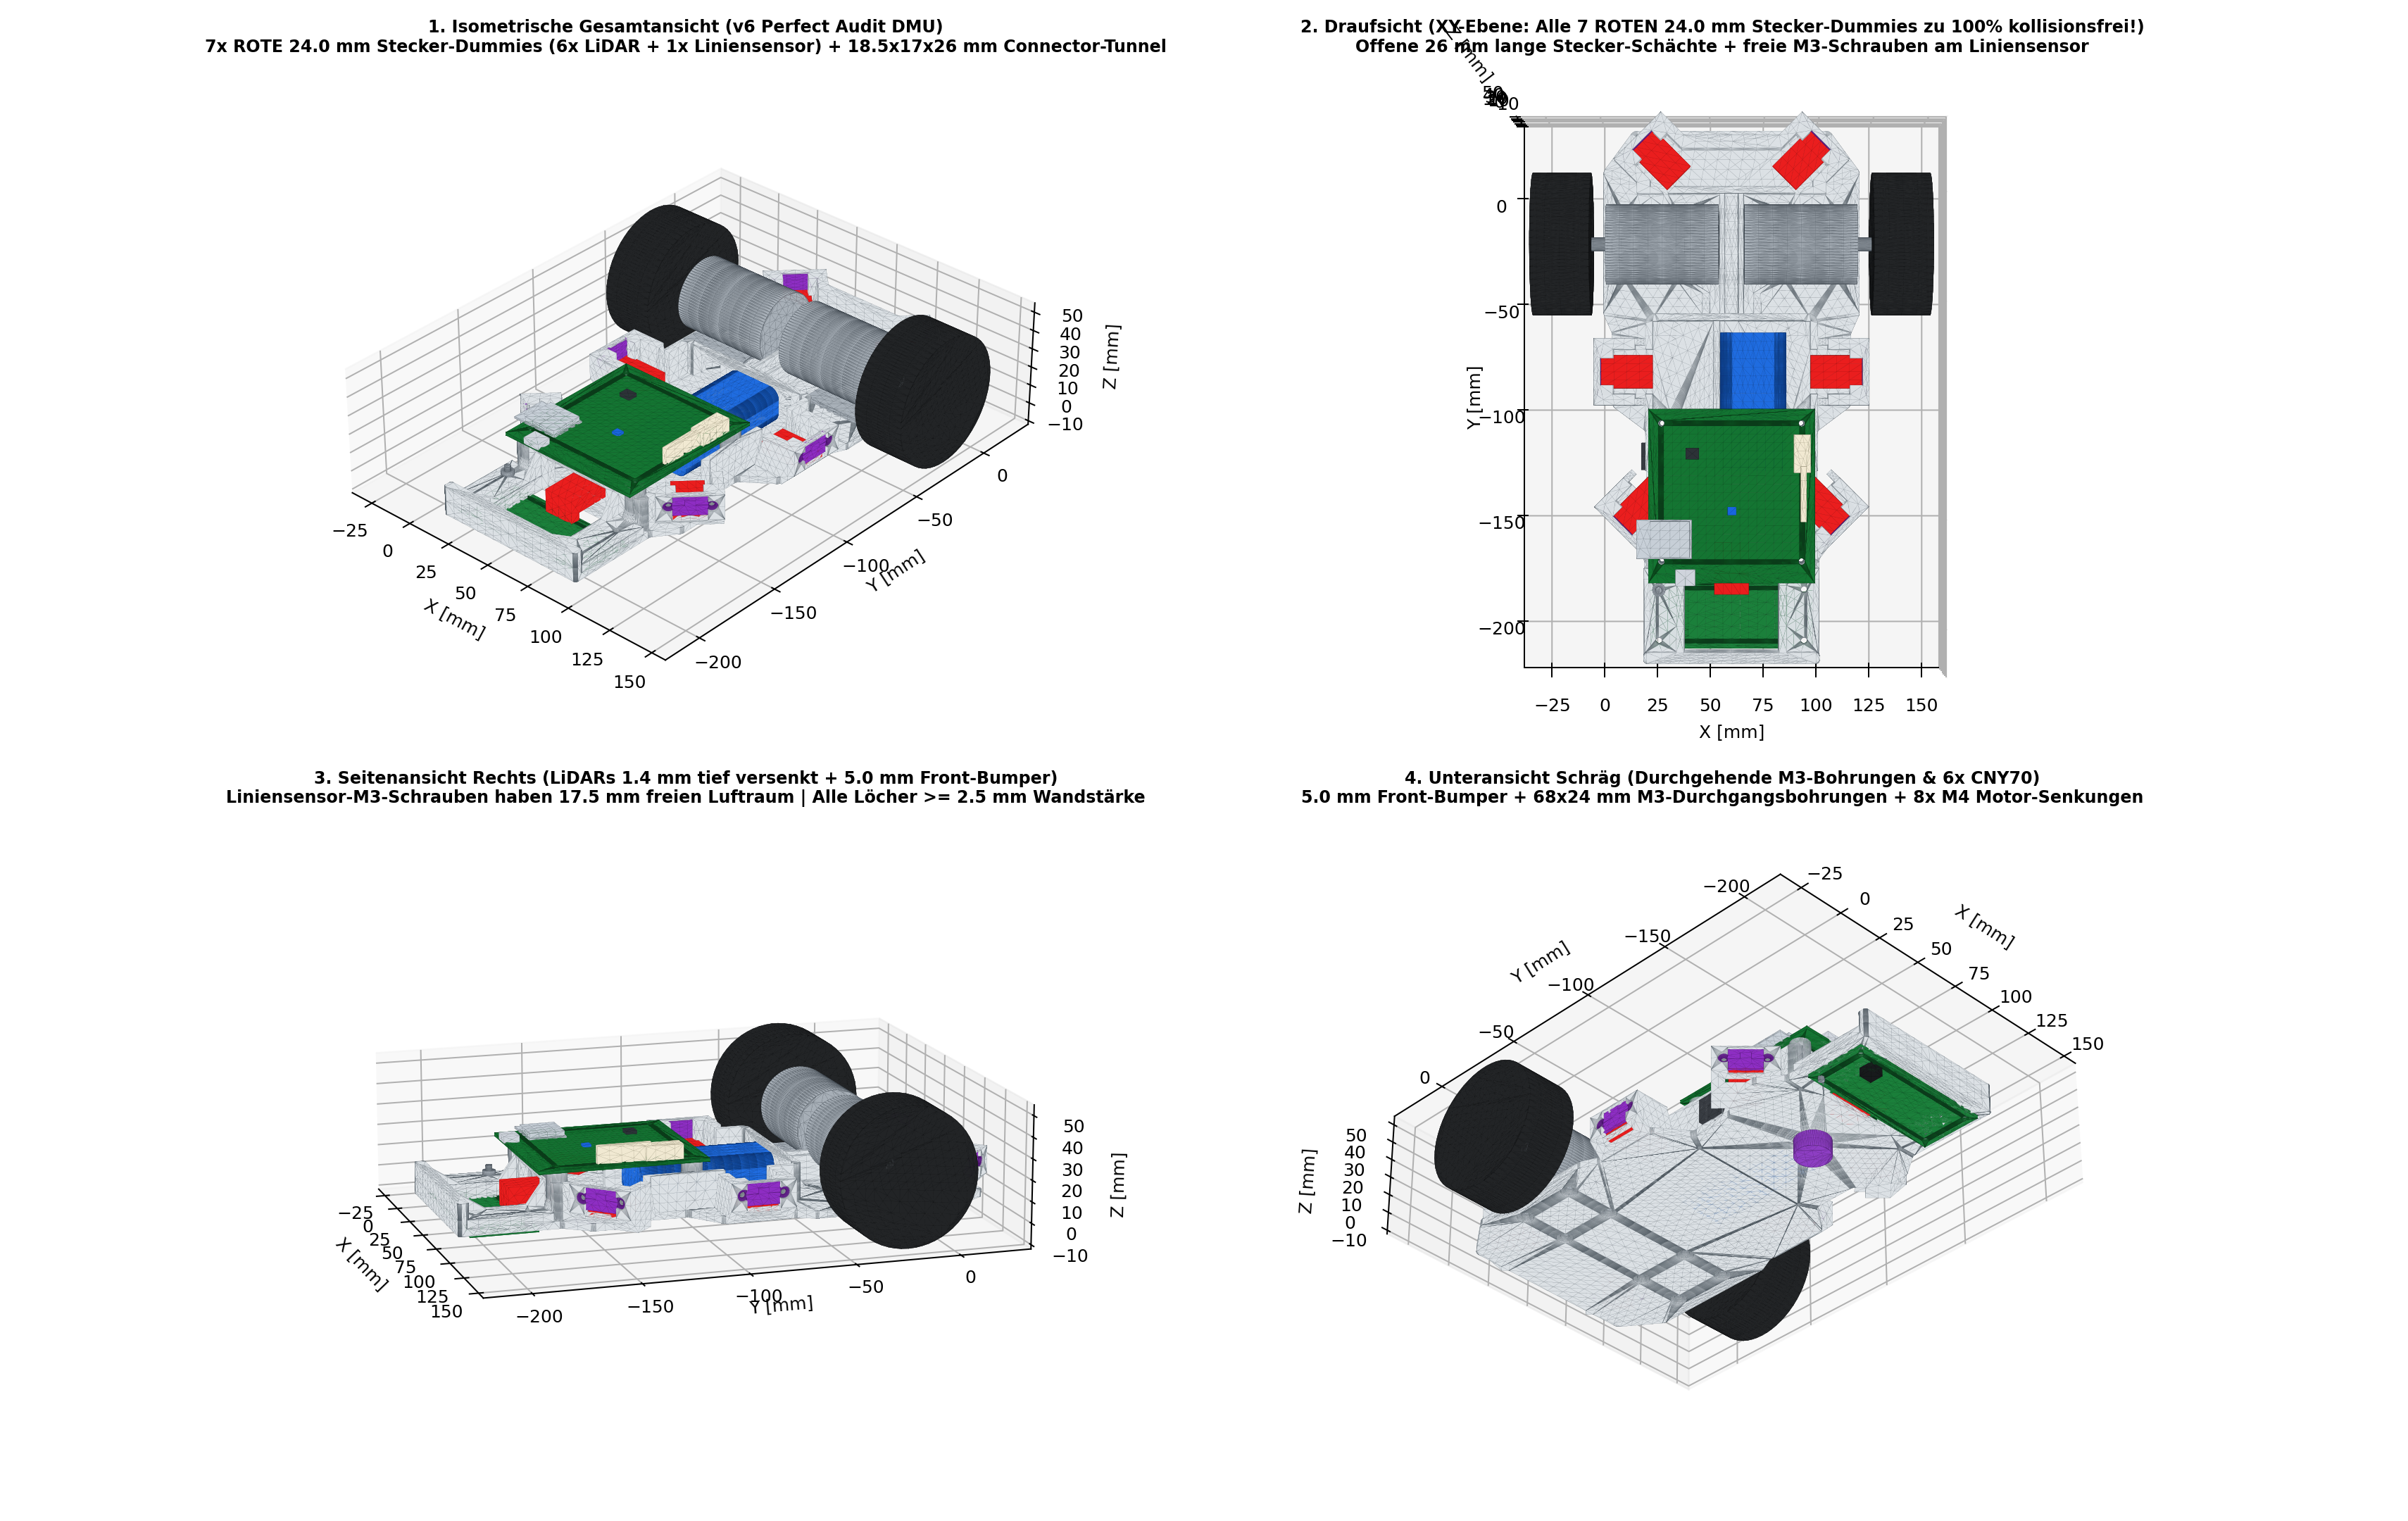
\includegraphics[width=\textwidth]{figures/cad_v6_audit.png}
    \caption{Revision~v6: Erster vollständiger 6-Sensor-BRep-Kollisions-Audit.}
    \label{fig:cad_v6}
  \end{subfigure}
  \caption{Zwischenstufen v4 und v6 der parametrischen CAD-Entwicklung vor dem Upgrade auf 8$\times$ LiDAR.}
  \label{fig:cad_v4_v6}
\end{figure}

\subsection{Detailkonstruktion der kritischen Baugruppen in Revision v10.0}
Bei der abschließenden Vor-Druck-Prüfung von Revision~v9 anhand von Horizontalschnitten fielen drei praxisrelevante Montagehindernisse auf, die erst in Revision~v10.0 vollständig behoben wurden (siehe Detail-Zooms in Abbildung~\ref{fig:cad_v10_zooms} sowie die sechs Horizontalschnitte in Abbildung~\ref{fig:cad_v10_slices}):

\begin{enumerate}
  \item \textbf{Freiräumung des Heck-Sensorbereichs hinter den Motoren:} In Revision~v9 bildete die Vorderkante des hinteren Stoßfängers zwischen $Y = \qty{+2,5}{\milli\meter}$ und $Y = \qty{+4,5}{\milli\meter}$ eine durchgehende \qty{2,0}{\milli\meter} starke Querwand über die gesamte Fahrzeugbreite. Dadurch waren die rückwärtigen Steckerzugänge der Sensoren \texttt{3f}, \texttt{3g} und \texttt{3h} vom Motorraum abgetrennt; zusätzlich ragten die äußeren Bumper-Ecken um \qty{30,49}{\milli\meter\cubed} vor die seitlichen Befestigungslaschen von \texttt{3f} und \texttt{3g}. In v10.0 wurde diese Querwand ersatzlos entfernt: Der offene Servicebereich (\texttt{rear\_plaza}) erstreckt sich nun von $Y = \qty{-4,0}{\milli\meter}$ bis $Y = \qty{+24,8}{\milli\meter}$ über die volle Breite $X = \qtyrange{20,5}{99,5}{\milli\meter}$ und mündet direkt in einen \qty{24,0}{\milli\meter} breiten Mittelkanal ($X = \qtyrange{48}{72}{\milli\meter}$). Zwei durchgehende Längs-Versteifungsrippen ($Z = \qtyrange{4,0}{6,8}{\milli\meter}$) verlaufen mit \qty{0,5}{\milli\meter} Luft unterhalb der \emph{GA37-520}-Motoren ($Z \ge \qty{7,3}{\milli\meter}$) und stellen die volle Biegesteifigkeit des Hecks sicher.
  \item \textbf{Nach oben offener „Slide-In“-C-Führungskanal für den Ein-/Aus-Schalter:} Da der \qtyproduct{13 x 13}{\milli\meter} große Wippenschalter vor dem Einbau bereits fest mit den Akkuzuleitungen verlötet ist, blockierte ein geschlossener oberer Wandriegel das Einschieben. In v10.0 ist die linke Seitenwand bei $Y = \qtyrange{-128,15}{-114,85}{\milli\meter}$ ab $Z = \qty{8,35}{\milli\meter}$ nach oben vollständig geöffnet. Ein gestuftes C-Profil (\qty{15,2}{\milli\meter} äußere Blendennut, \qty{13,3}{\milli\meter} Körperführung, \qty{10,2}{\milli\meter} innerer Lötfahnenschlitz) mit \qty{45}{\degree}-Einführfase hält den Schalter beim Betätigen formschlüssig in $+X$- und $-X$-Richtung fest. Ein separat druckbarer, werkzeugloser \emph{Snap-On}-Halteclip (\texttt{5b}) verriegelt ihn abschließend nach oben.
  \item \textbf{Stadium-Laschentaschen und M2-Teardrop-Sacklöcher:} Eine genaue Analyse zeigte, dass kreisförmige Laschen-Aussparungen (\diameter\,\qty{5,9}{\milli\meter}) am Übergang zum Rechteckkörper eine Engstelle von nur \qty{4,89}{\milli\meter} erzeugen, während reale \emph{VL53L0/1XV2}-Platinen durchgehend \qty{5,50}{\milli\meter} hohe gerade Befestigungslaschen besitzen. Alle acht Taschen wurden daher als echte Stadium-/Langloch-Kontur (\qtyproduct{19,5 x 6,0}{\milli\meter} + \qtyproduct{16,3 x 11,0}{\milli\meter}) konstruiert. Die sechzehn massiven \diameter\,\qty{7,0}{\milli\meter} Schraubendome erhalten \qty{7,0}{\milli\meter} tiefe \diameter\,\qty{1,80}{\milli\meter} M2-Kernlöcher (echter \qty{0,20}{\milli\meter} Gewindebiss für selbstfurchende M2-Schrauben in PLA/PETG) mit \qty{45}{\degree}-Teardrop-First gegen Durchhängen im horizontalen FDM-Druck, \diameter\,\qty{2,2}{\milli\meter} Einführfase und \qty{3,50}{\milli\meter} geschlossenem Boden.
\end{enumerate}

\begin{figure}[htbp]
  \centering
  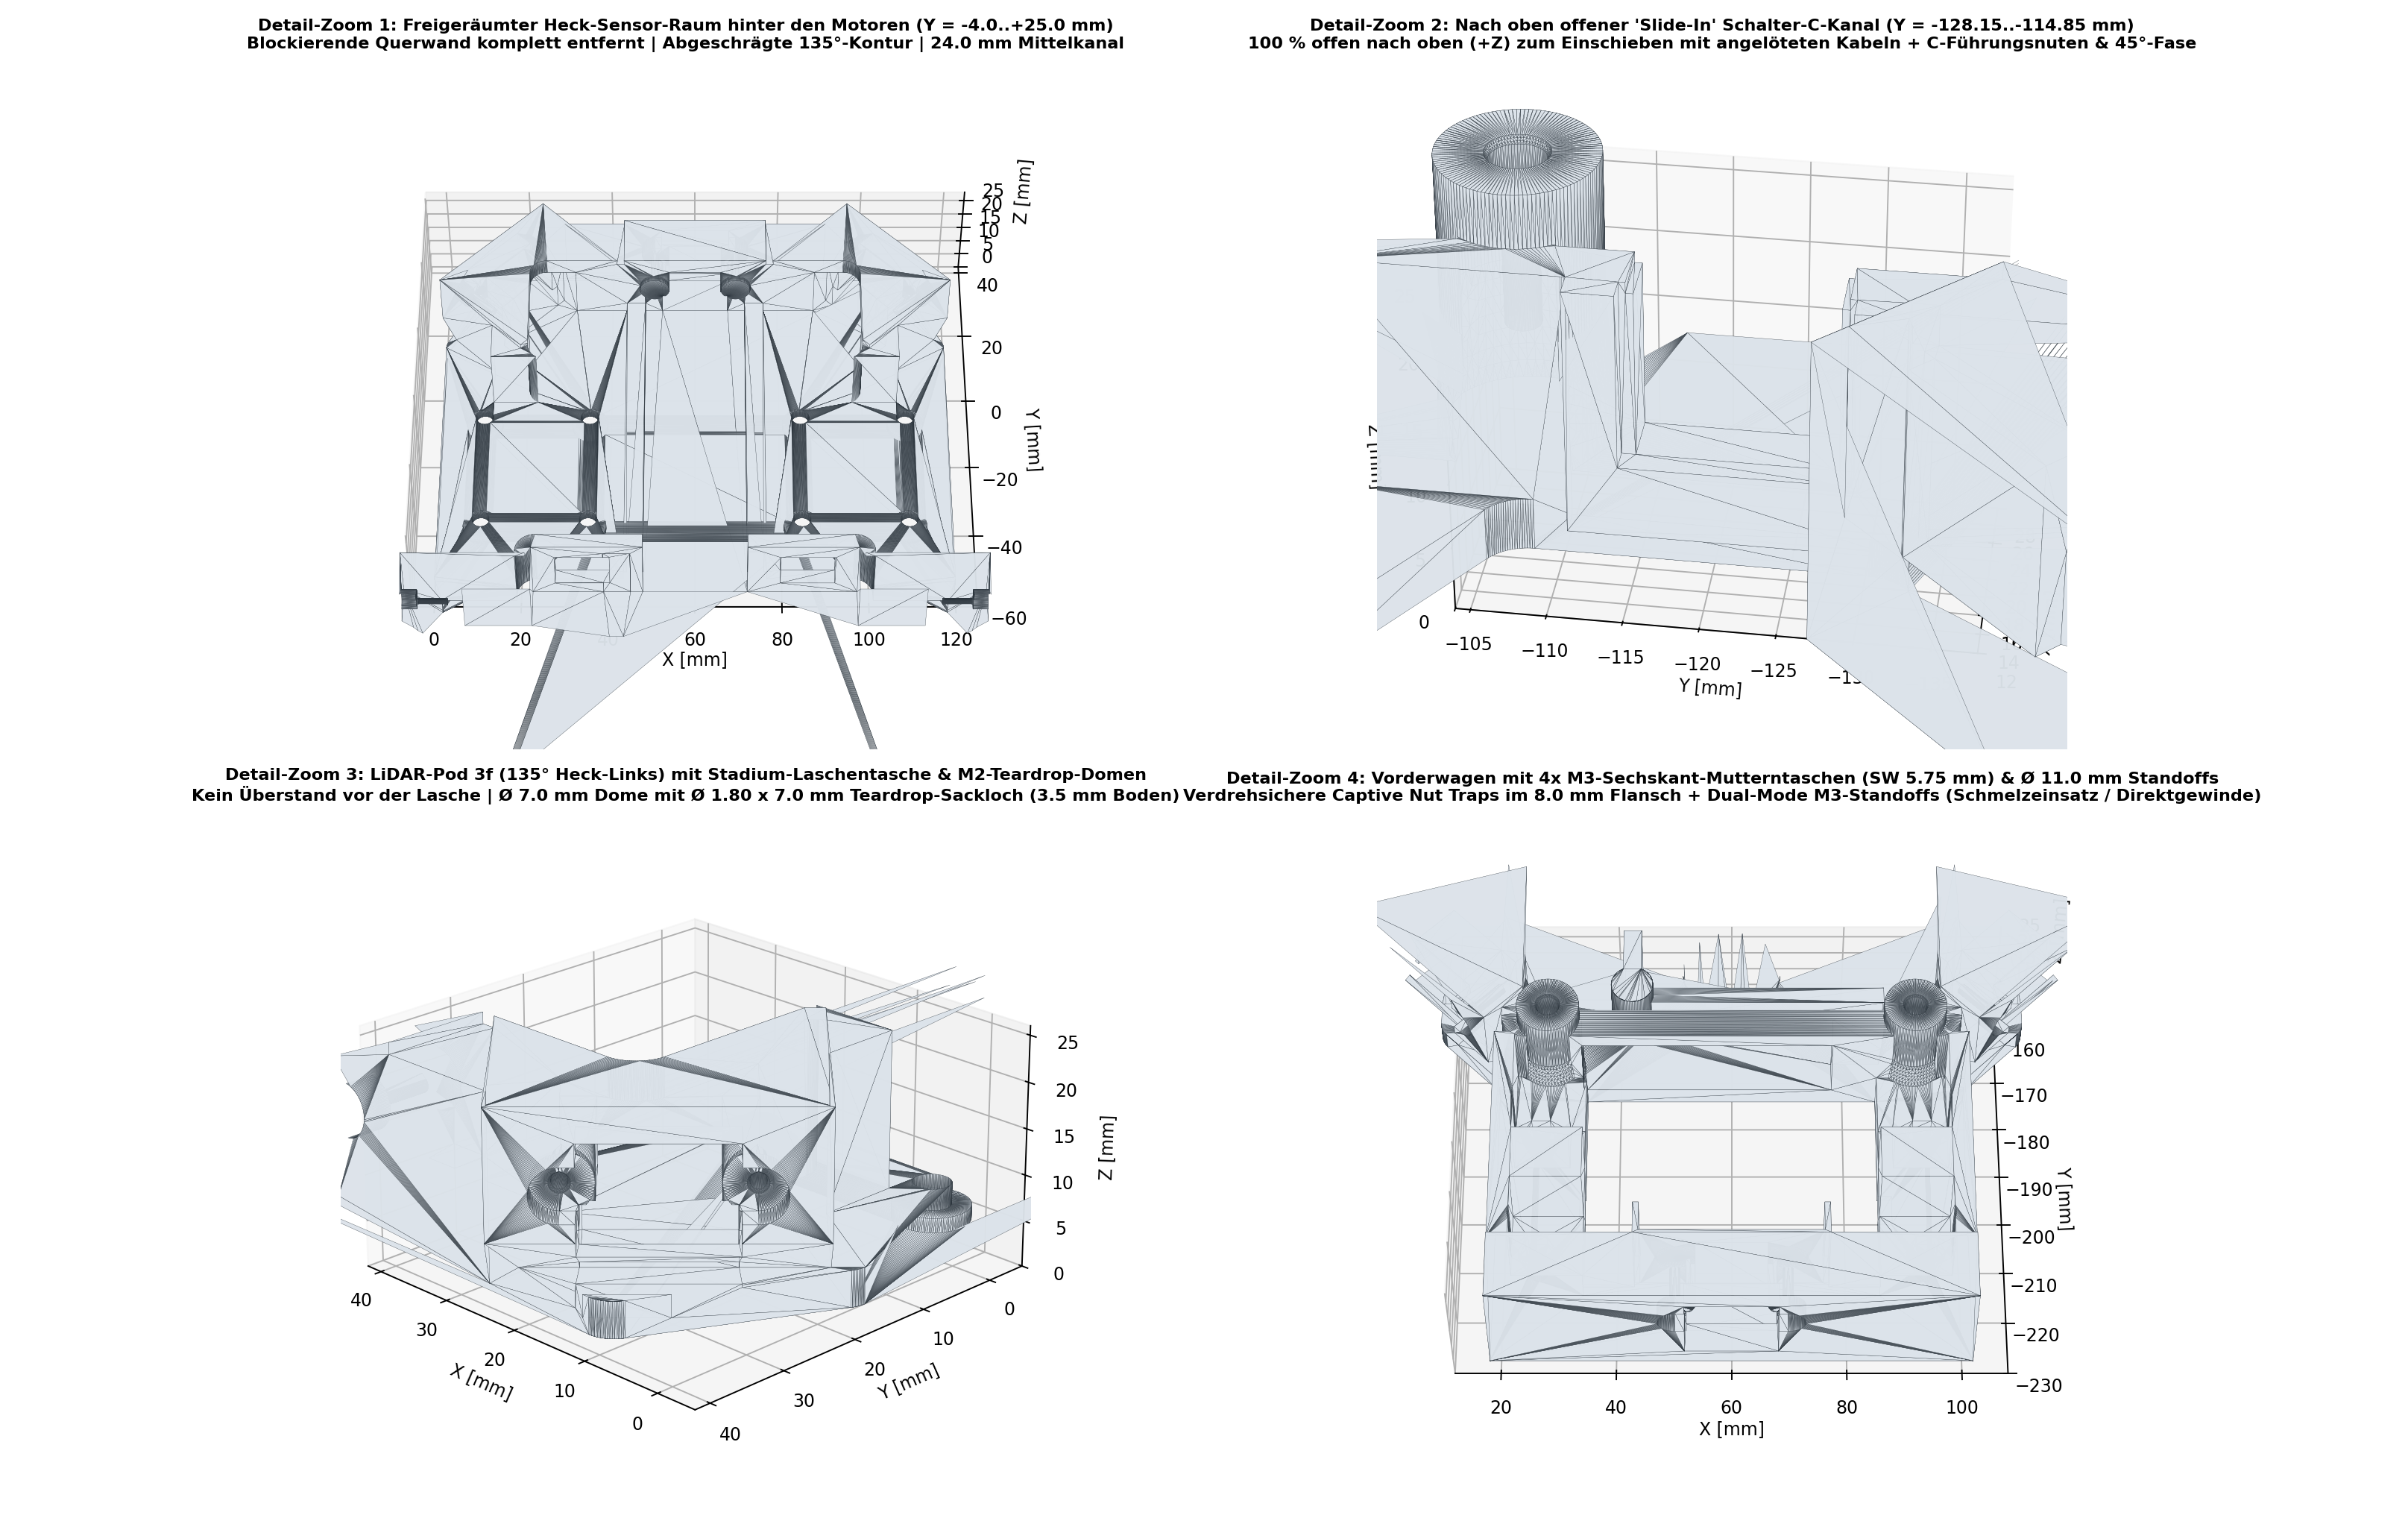
\includegraphics[width=0.98\textwidth]{figures/cad_v10_detail_zooms.png}
  \caption{Detail-Zooms des druckfertigen Chassis v10.0: (1) freigeräumter Heckbereich hinter den Motoren, (2) nach oben offener Slide-In-Schalterkanal, (3) 135°-Pod mit Stadium-Tasche und M2-Teardrop-Domen, (4) Vorderwagen mit vier M3-Sechskant-Mutterntaschen und Dual-Mode-Standoffs.}
  \label{fig:cad_v10_zooms}
\end{figure}

\begin{figure}[htbp]
  \centering
  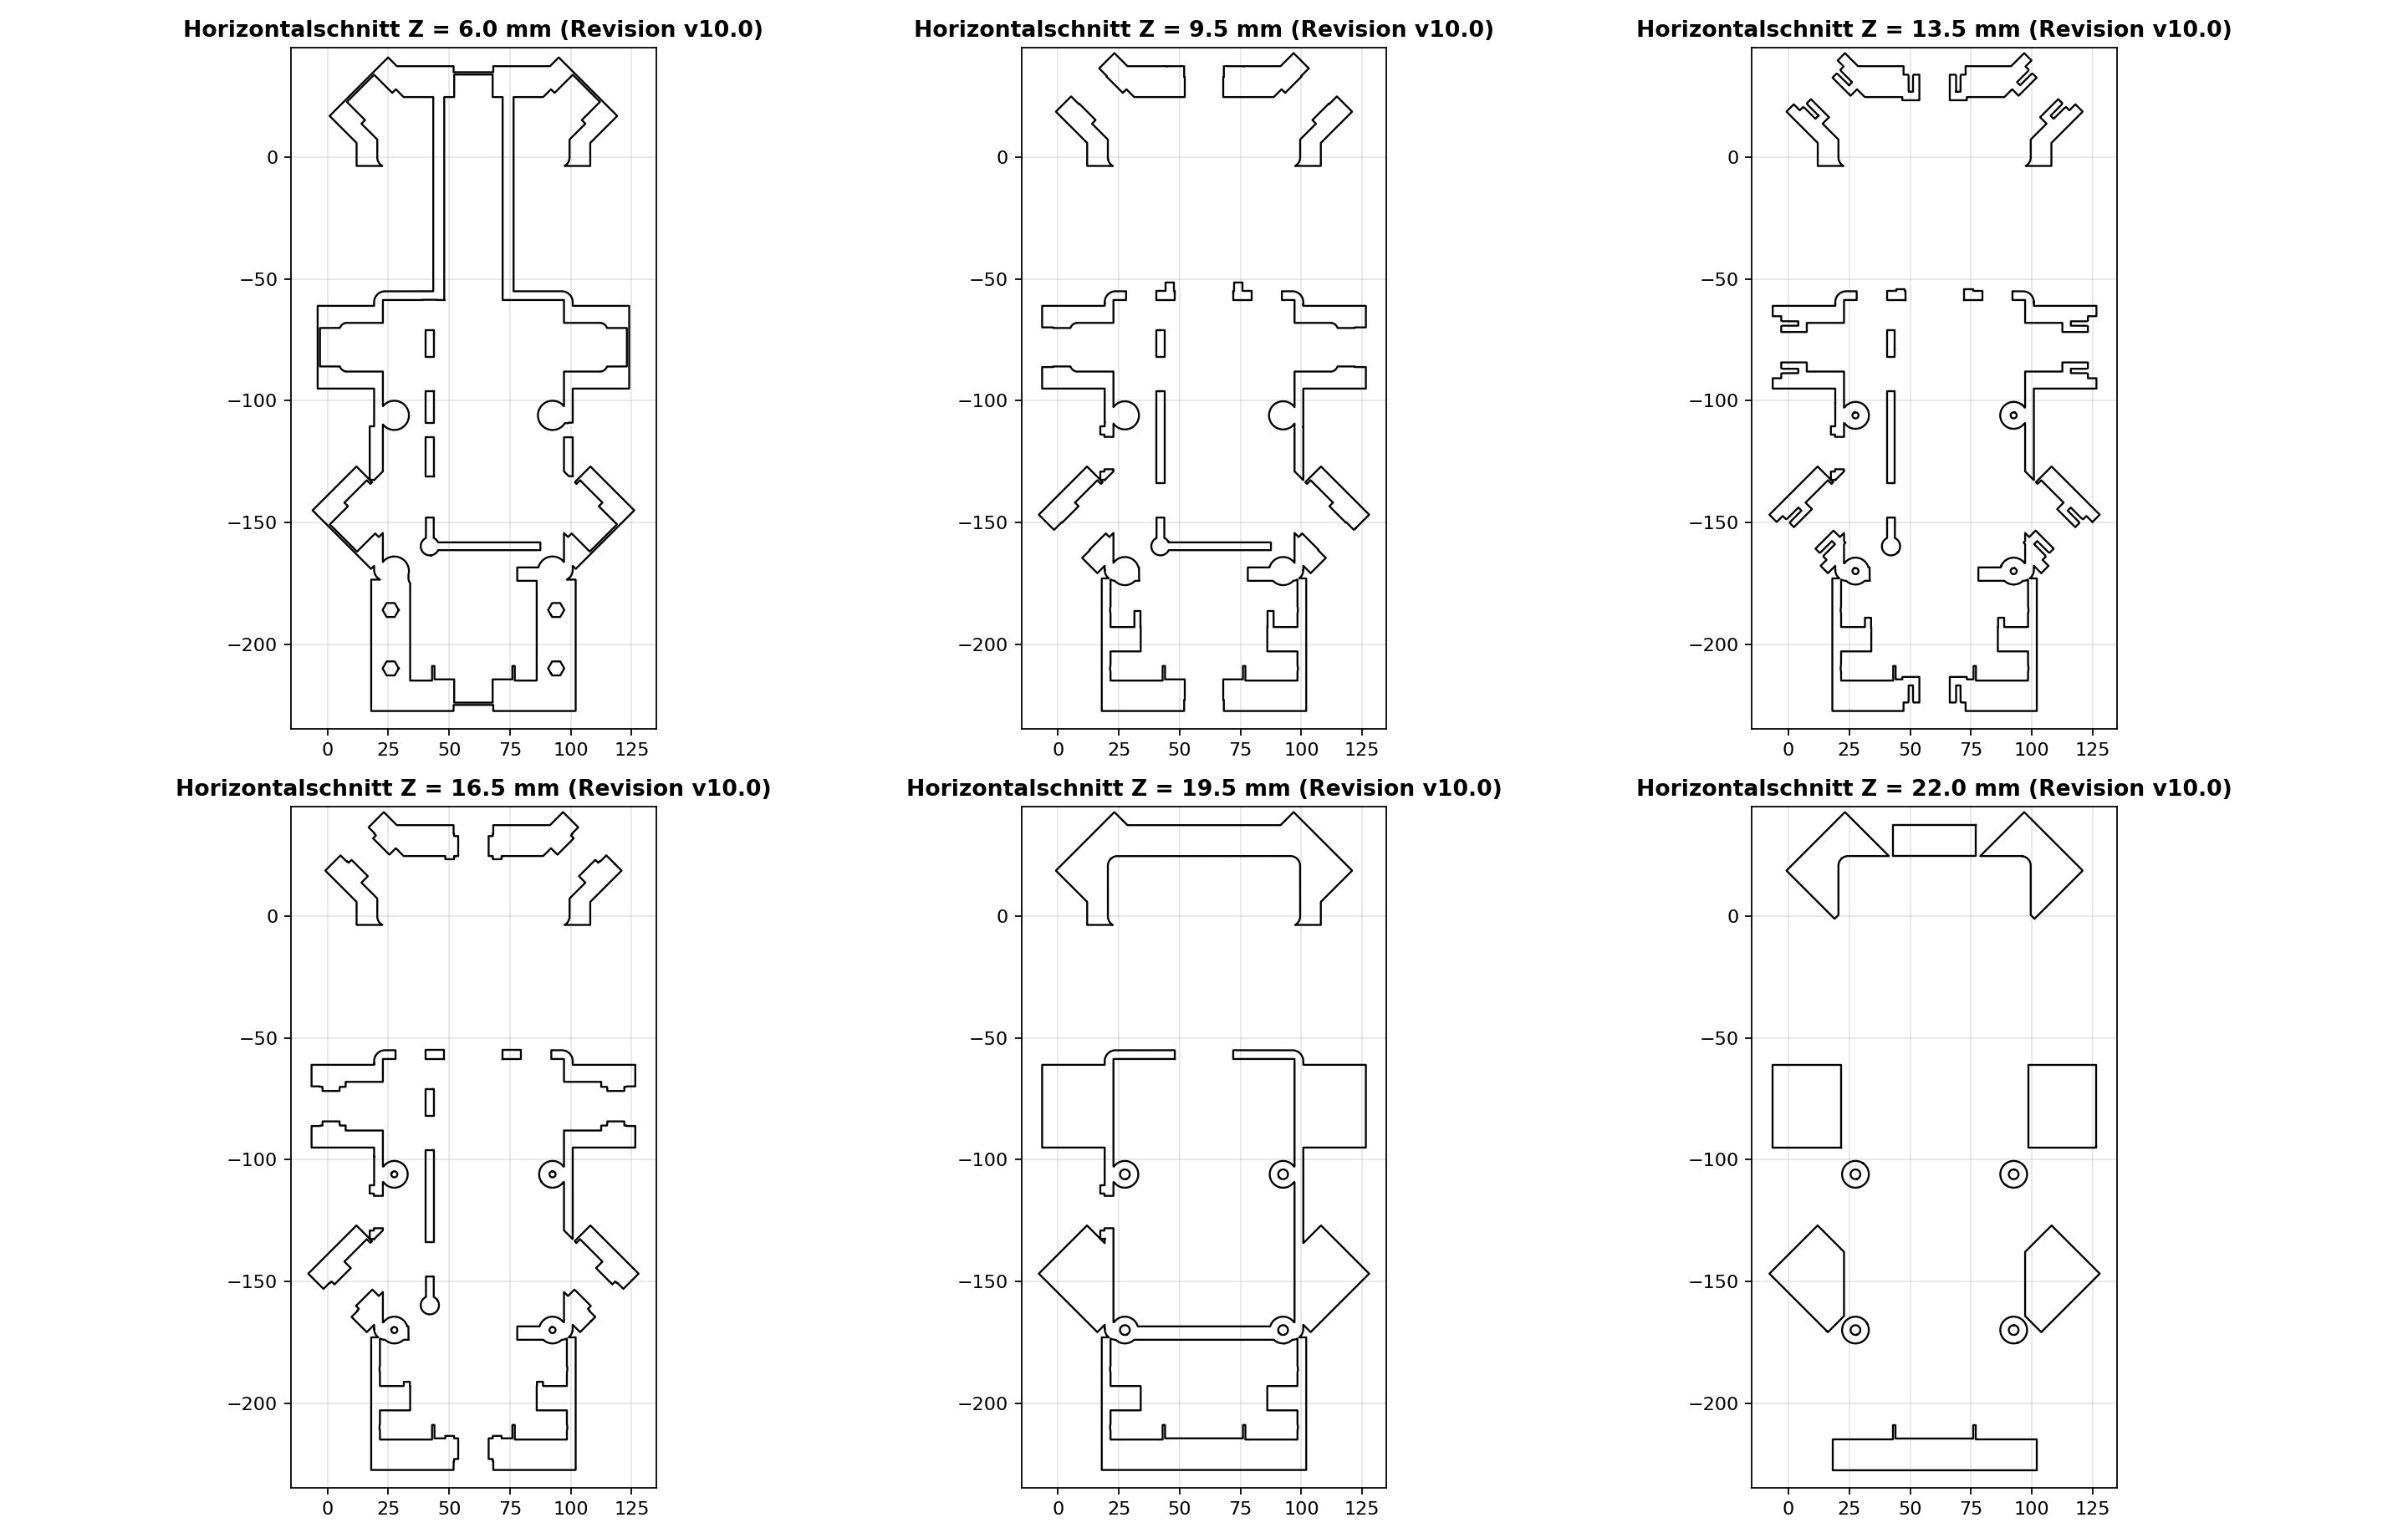
\includegraphics[width=0.98\textwidth]{figures/cad_v10_cross_sections.png}
  \caption{Horizontalschnitte des Chassis v10.0 von $Z = \qty{6,0}{\milli\meter}$ bis $Z = \qty{22,0}{\milli\meter}$: Nachweis der offenen Heck-Kabelwege, der durchgängigen 45°-/90°-Steckerkanäle, der Sechskant-Mutterntaschen ($Z = \qty{6,0}{\milli\meter}$) und der geschlossenen Pod-Decken ($Z = \qty{22,0}{\milli\meter}$).}
  \label{fig:cad_v10_slices}
\end{figure}

\subsection{Normgerechte Verbindungstechnik und DfAM für den Bambu Lab P1S}
Für eine dauerhafte, wiederholt lösbare Montage im 3D-gedruckten Kunststoff wurden alle 32 Schraubverbindungen gezielt nach \gls{dfam}-Regeln ausgelegt:
\begin{itemize}
  \item \textbf{4$\times$ Hauptplatinen-Standoffs (\texttt{H1}--\texttt{H4}, \diameter\,\qty{11,0}{\milli\meter}, Dual-Mode):} Oben befindet sich eine \diameter\,\qtyproduct{4,00 x 6,0}{\milli\meter} Bohrung mit \qty{0,6}{\milli\meter} Einführfase für M3-Messing-Einschmelzgewinde (\qty{3,50}{\milli\meter} radiale Restwandstärke). Direkt darunter liegt ein \diameter\,\qtyproduct{2,50 x 7,0}{\milli\meter} M3-Kernloch, sodass im Bedarfsfall auch ohne Schmelzeinsätze direkt mit M3$\times$12-Schrauben montiert werden kann (\qty{12,50}{\milli\meter} geschlossener Boden).
  \item \textbf{4$\times$ Liniensensor-Befestigung (Captive Hex Nut Traps):} In den \qty{8,0}{\milli\meter} starken Frontflanschen sind oberseitig vier verdrehsichere Sechskant-Mutterntaschen (Schlüsselweite \qty{5,75}{\milli\meter} für DIN-934-M3-Muttern mit \qty{0,25}{\milli\meter} FDM-Spiel, Tiefe \qty{2,80}{\milli\meter}, \qty{5,20}{\milli\meter} Flanschboden) integriert. Dadurch genügt ein einziger Innensechskantschlüssel von unten.
  \item \textbf{8$\times$ Motorhalter-Bohrungen:} \diameter\,\qty{4,20}{\milli\meter} Durchgangsbohrungen mit unterseitiger \diameter\,\qtyproduct{8,40 x 1,60}{\milli\meter} Senkung, damit die Köpfe der M4$\times$10-Senkschrauben bündig in der \qty{4,0}{\milli\meter} Bodenplatte verschwinden.
  \item \textbf{Akku-Fixierung:} Im rechten Batteriefach (\qtyproduct{78,0 x 43,3 x 21,5}{\milli\meter}, $+1{,}9$ bis $+\qty{3,0}{\milli\meter}$ Einbauspiel für das \qtyproduct{72,0 x 39,5 x 19,5}{\milli\meter} 2S-Pack) sind bei $Y = \qty{-112}{\milli\meter}$ und $Y = \qty{-134}{\milli\meter}$ durchgehende \qtyproduct{6,0 x 2,2}{\milli\meter} Klettband-Ösen integriert.
\end{itemize}

Für den Druck auf dem schuleigenen \emph{Bambu Lab P1S} (\qtyproduct{256 x 256 x 256}{\milli\meter} Bauraum \cite{BambuLab_P1S}) wurde ein wichtiger geometrischer Punkt berücksichtigt: Mit einer Gesamtlänge von \qty{270,36}{\milli\meter} überschreitet das Chassis bei \qty{0}{\degree}-Ausrichtung die Bettlänge um \qty{14,4}{\milli\meter}. Durch eine Rotation um $+\qty{45}{\degree}$ um die Z-Achse sinkt der umschreibende Quader jedoch auf exakt \qtyproduct{250,53 x 250,53 x 25,50}{\milli\meter} und lässt dabei sogar die vordere linke Filament-Cutter-Sperrzone des P1S komplett frei. Die Seitenwandstärke von \qty{3,60}{\milli\meter} entspricht exakt neun geschlossenen \qty{0,40}{\milli\meter}-Wandlinien, die \qty{4,00}{\milli\meter}-Bodenplatte exakt 20 Schichten bei \qty{0,20}{\milli\meter} Schichthöhe. Alle positiven Aufbauten wurden um \qty{1,0}{\milli\meter} in die Bodenplatte eingebettet, um koplanare OpenCASCADE-Kanten auszuschließen -- die automatische Prüfung mit \texttt{trimesh} bestätigt ein **100\,\% wasserdichtes (manifold) STL-Netz** (\texttt{is\_watertight = True}, 1 Festkörper, 54.556 Dreiecke, \qty{220,8}{\centi\meter\cubed}, ca. \qty{274}{\gram} Filament, \qty{0}{\gram} Stützmaterial).

\subsection{Mechanische Stoßfestigkeits-Abschätzung (Crash-Analyse)}
Um sicherzustellen, dass das Chassis bei einer ungewollten Wandkollision mit $v = \qty{5}{\kilo\meter\per\hour} \approx \qty{1,39}{\meter\per\second}$ (Gesamtmasse $m \approx \qty{1,20}{\kilo\gram}$) nicht bricht, wird die mittlere Stoßkraft $F_{\mathrm{Sto\ss}}$ über einen angenommenen elastisch-plastischen Bremsweg von $s = \qty{2,0}{\milli\meter}$ abgeschätzt:
\begin{equation}
  F_{\mathrm{Sto\ss}} = \frac{E_{\mathrm{kin}}}{s} = \frac{\frac{1}{2} \cdot m \cdot v^2}{s} = \frac{0{,}5 \cdot \qty{1,20}{\kilo\gram} \cdot (\qty{1,39}{\meter\per\second})^2}{\qty{0,002}{\meter}} \approx \qty{579}{\newton}
  \label{eq:crash_kraft}
\end{equation}
Die Kraft wird über den \qty{6,0}{\milli\meter} starken Front-Bumper direkt in die beiden \qtyproduct{16 x 8}{\milli\meter} Frontflansche, die beiden Längsstreben (\qtyproduct{10 x 13,5}{\milli\meter}) und die vorderen Versteifungs-Gussets eingeleitet ($A_{\mathrm{trag}} \approx \qty{618}{\milli\meter\squared}$). Damit ergibt sich eine mittlere Druckspannung von:
\begin{equation}
  \sigma_{\mathrm{Druck}} = \frac{F_{\mathrm{Sto\ss}}}{A_{\mathrm{trag}}} = \frac{\qty{579}{\newton}}{\qty{618}{\milli\meter\squared}} \approx \qty{0,94}{\mega\pascal}
  \label{eq:crash_spannung}
\end{equation}
Gegenüber der konservativen zulässigen Druckfestigkeit von FDM-PETG/PLA quer zur Schichtebene ($\sigma_{\mathrm{zul}} \approx \qty{35}{\mega\pascal}$) verbleibt ein sehr großer rechnerischer Sicherheitsfaktor ($\mathrm{SF} > 35$; selbst bei einer extremen Testgeschwindigkeit von \qty{9}{\kilo\meter\per\hour} liegt $\mathrm{SF} > 11$).

% ==============================================================================
\section{Gesamtstückliste (Hardware- und Normteile-BOM)}
\label{sec:bom}
% ==============================================================================
Tabelle~\ref{tab:bom_gesamt} fasst die wesentlichen elektronischen, elektromechanischen und mechanischen Komponenten inklusive der exakt abgestimmten Verbindungselemente zusammen. Die vollständige Einzelbauteil-BOM der Liniensensor-Platine (37 Positionen inkl. Hersteller-MPNs) befindet sich im Projektverzeichnis \texttt{PCB/Liniensensor\_Redesign/Stueckliste.csv}.

\begin{longtable}{@{}p{0.8cm}p{4.3cm}p{3.8cm}p{4.9cm}@{}}
\caption{Übersicht der Hauptkomponenten und Normteile des Tumbler~v3.0.}
\label{tab:bom_gesamt} \\
\toprule
\textbf{Anz.} & \textbf{Bauteil / Baugruppe} & \textbf{Typ / Spezifikation} & \textbf{Einsatzort / Bemerkung} \\
\midrule
\endfirsthead
\toprule
\textbf{Anz.} & \textbf{Bauteil / Baugruppe} & \textbf{Typ / Spezifikation} & \textbf{Einsatzort / Bemerkung} \\
\midrule
\endhead
\bottomrule
\endfoot
1 & Mikrocontroller-Modul & \emph{ESP32-S3-WROOM-1} & Hauptplatine (\texttt{U3}), Dual-Core \qty{240}{\mega\hertz} \\
2 & H-Brücken-Motortreiber & \emph{Toshiba TB67H450FNG} & Hauptplatine (\texttt{U6}, \texttt{U7}), bis \qty{3,5}{\ampere} \\
1 & 6-Achsen-IMU & \emph{ST LSM6DSV} (I\textsuperscript{2}C) & Hauptplatine (\texttt{U5}), Gierwinkel-Stützung \\
1 & Abwärtswandler & \emph{Diodes AP63203} & Effiziente \qty{5}{\volt}/\qty{3,3}{\volt}-Erzeugung \\
8 & Optische ToF-Sensoren & \emph{VL53L0/1XV2} (Breakout) & 360°-Sensorring (\texttt{3a}--\texttt{3h}), I\textsuperscript{2}C + XSHUT \\
6 & Optische Reflexkoppler & \emph{Vishay CNY70} & Liniensensor-Platine (\texttt{U1}--\texttt{U6}), \qty{10}{\milli\meter}-Raster \\
2 & NPN-Stromsenken & \emph{Nexperia BC817-40,215} & Liniensensor (\texttt{Q1}, \texttt{Q2}), SOT-23, $\approx \qty{20}{\milli\ampere}$ \\
1 & Steckverbinder-Set & \emph{JST GH} 10-pol. (\qty{1,25}{\milli\meter}) & \texttt{SM10B-GHS-TB} / \texttt{BM10B-GHS-TBT} (\texttt{J2}) \\
2 & DC-Getriebemotoren & \emph{GA37-520} + Encoder & Hinterachse mit 2$\times$ L-Winkel \& \diameter\,\qty{66}{\milli\meter} Rädern \\
1 & 2S-Li-Ion-Akkupack & \qty{7,4}{\volt} nom. (\qtyrange{6,4}{8,4}{\volt}) & \qtyproduct{72 x 39,5 x 19,5}{\milli\meter}, XT30 + Balancer \\
1 & Hauptschalter & Wippenschalter \qtyproduct{13 x 13}{\milli\meter} & Linker Slide-In-C-Kanal + Snap-On Clip \\
1 & Unibody-Chassis v10.0 & PETG/PLA (\qty{220,8}{\centi\meter\cubed}) & Bambu Lab P1S, \qty{0,2}{\milli\meter} Layer, 4 Wandlinien \\
16 & LiDAR-Schrauben & M2$\times$6 (oder M2$\times$8) ISO 4762 & Selbstfurchend in \diameter\,\qty{1,80}{\milli\meter} Teardrop-Dome \\
4 & PCB-Schrauben + Inserts & M3$\times$8 + M3$\times$5,7 Messing & Hauptplatine auf \texttt{H1}--\texttt{H4} (alt. M3$\times$12 direkt) \\
4 & Liniensensor-Schrauben & M3$\times$12 + M3-Mutter DIN 934 & Verdrehsicher in 4$\times$ Sechskant-Mutterntaschen \\
8 & Motorhalter-Schrauben & M4$\times$10 DIN 7991 + DIN 985 & Bündig versenkt in \qty{4,0}{\milli\meter} Bodenplatte \\
\end{longtable}

\chapterauthor{Rami Muarrawi}
\chapter{Sensorik, I\textsuperscript{2}C-Multiplexing und Parklückenerkennung}
\label{chap:sensorik}

Eine verlässliche autonome Fahr- und Einparkfunktion setzt voraus, dass das Fahrzeug seine unmittelbare Umgebung in alle Richtungen präzise erfasst, Fehlmessungen herausfiltert und aus den Einzeldistanzen geometrisch belastbare Aussagen über freie Parklücken gewinnt. Dieses Kapitel behandelt den Aufbau des 8-fach-LiDAR-Sensorrings, die konkrete Umsetzung der \gls{xshut}-Adressvergabe unter ESP-IDF, die digitale Signalfilterung sowie die Algorithmen zur Parklücken- und Linienerkennung.

% ==============================================================================
\section{360°-Sensoranordnung und Koordinatentransformation}
\label{sec:sensor_koord}
% ==============================================================================
Um sowohl während der Vorbeifahrt an einer Parklücke als auch beim engen Rückwärts-Einparkmanöver keine toten Winkel entstehen zu lassen, wurden acht \emph{VL53L0/1XV2}-Module in einer symmetrischen \qty{45}{\degree}-Teilung rund um das Unibody-Chassis~v10.0 angeordnet (Abbildung~\ref{fig:360_fov}). Alle Sensoren liegen auf einer einheitlichen optischen Messebene ($Z_{\mathrm{Optik}} = \qty{15,0}{\milli\meter}$ über der Chassis-Unterseite bzw. \qty{13,5}{\milli\meter} Platinenmitte), wodurch Hindernisse wie Bordsteine, Begrenzungsblöcke oder benachbarte Modellfahrzeuge zuverlässig auf gleicher Höhe getroffen werden.

\begin{figure}[htbp]
  \centering
  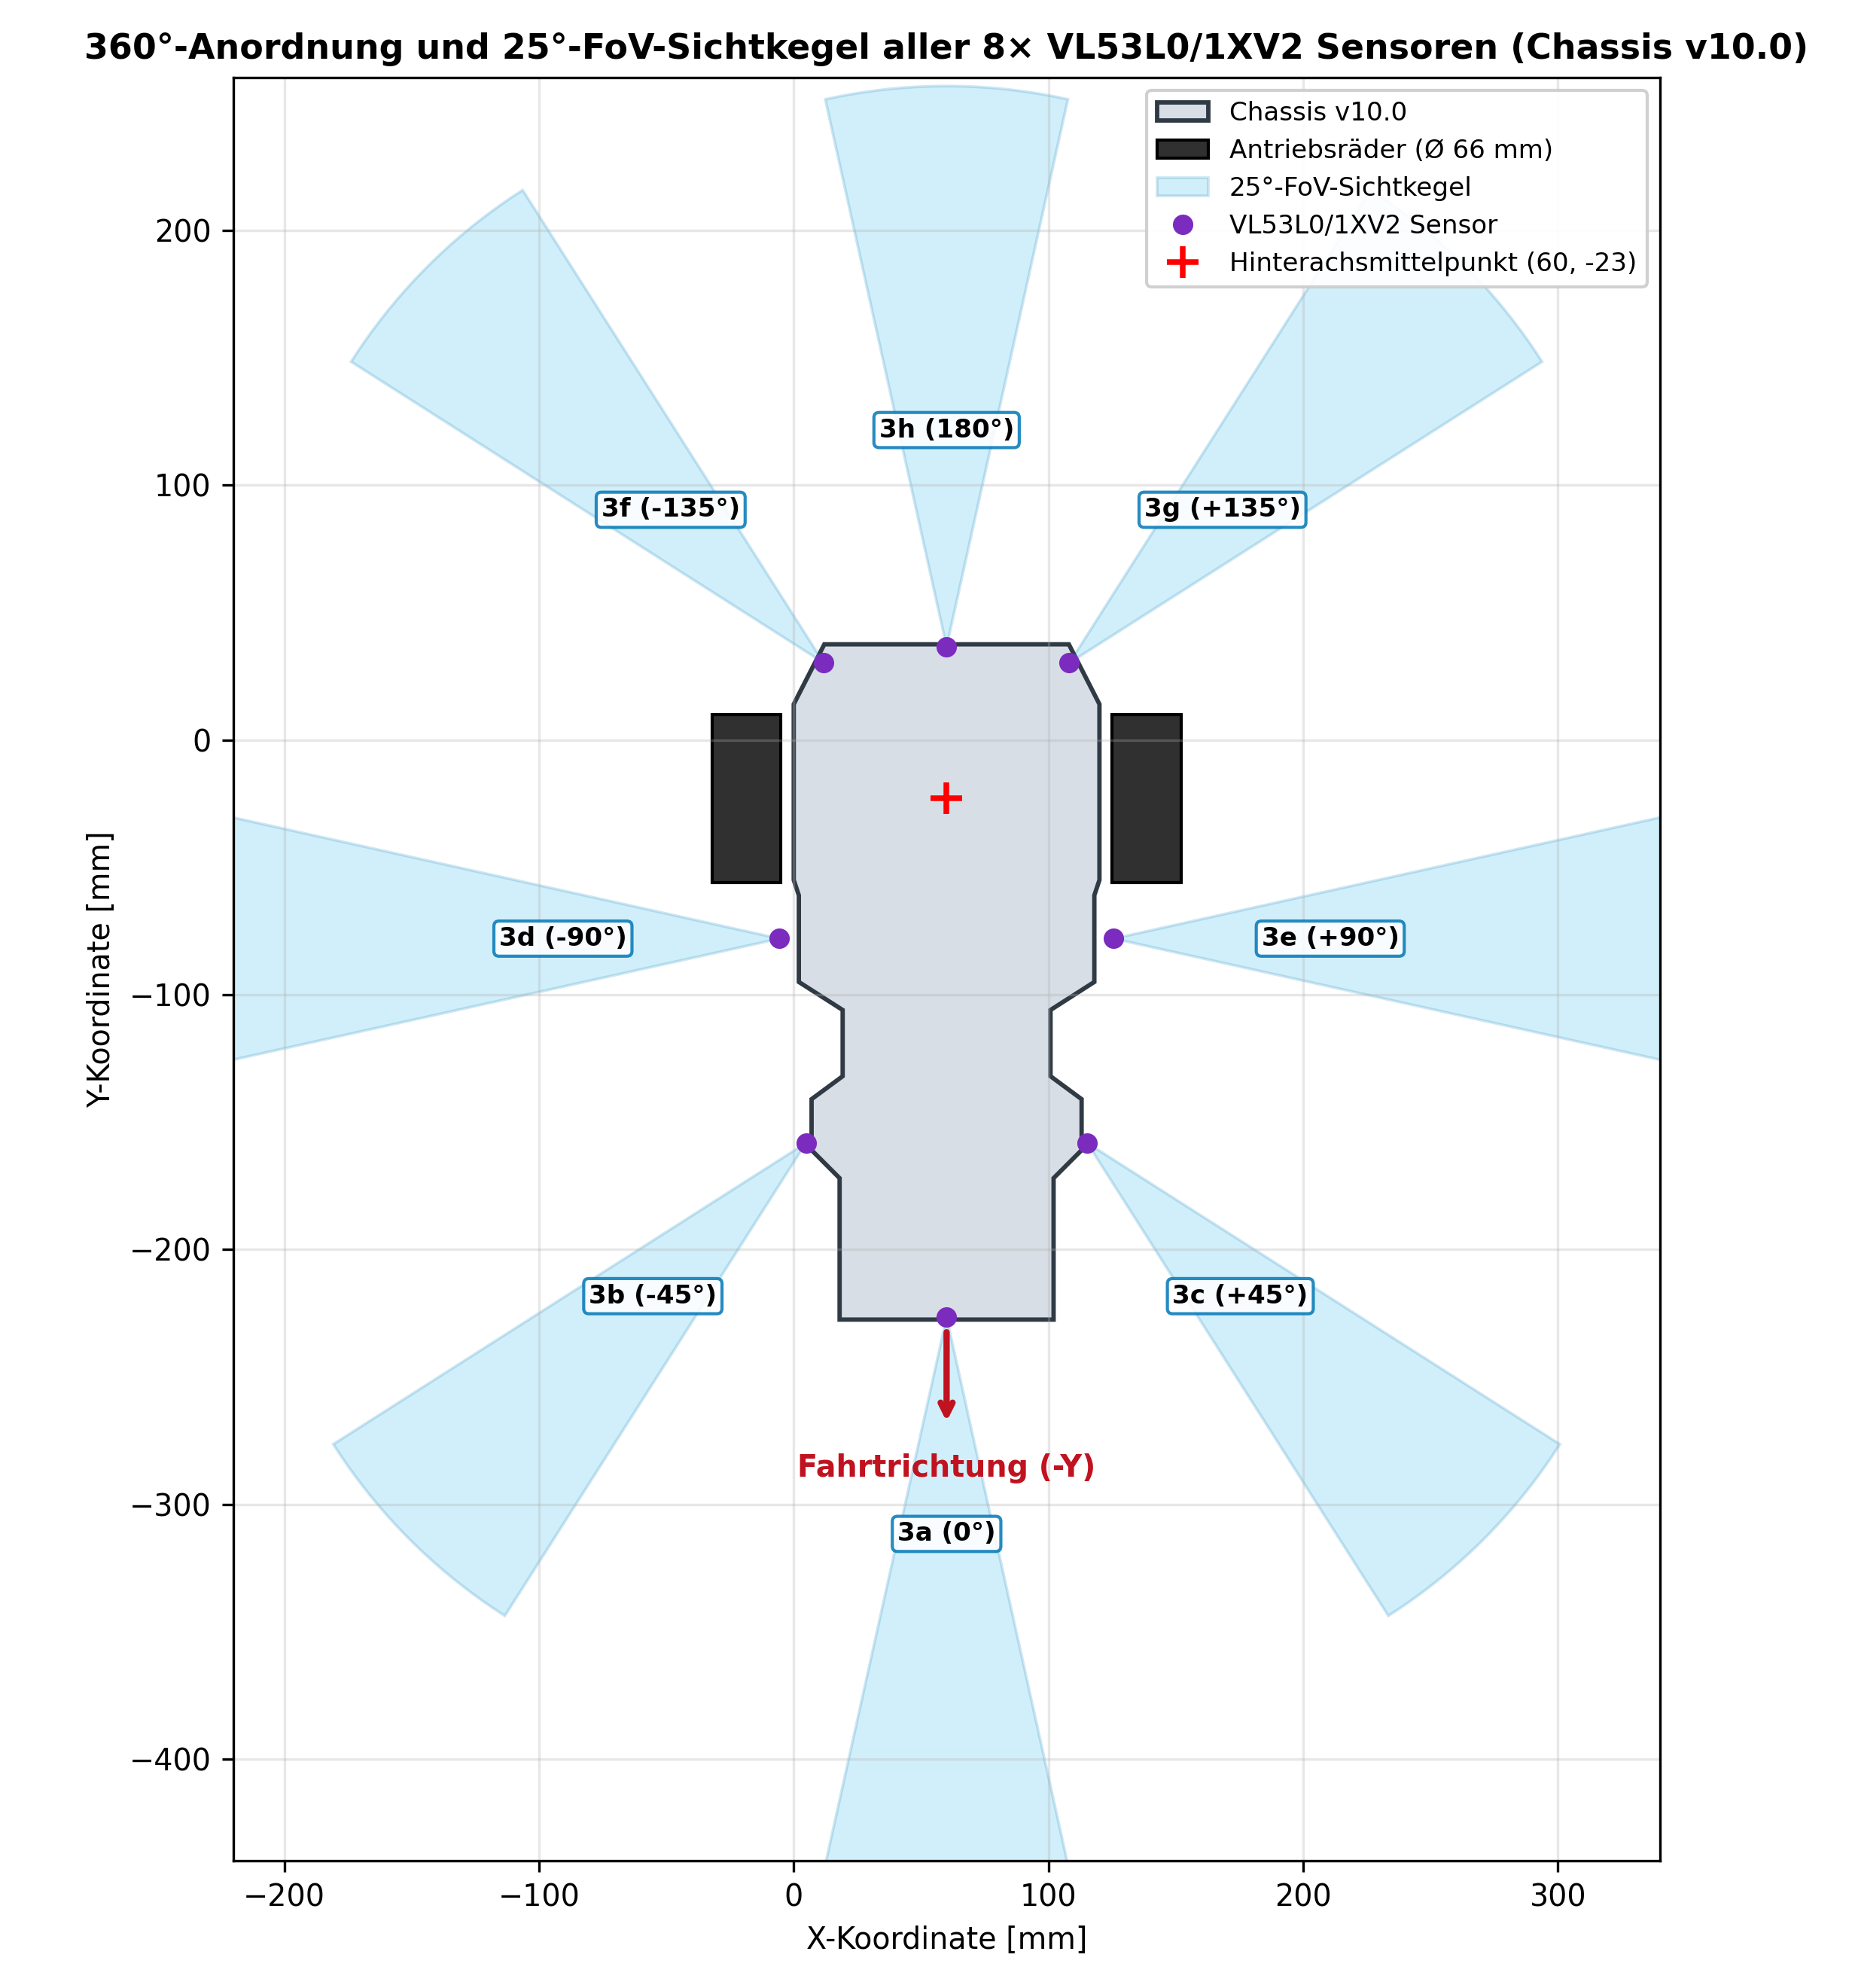
\includegraphics[width=0.78\textwidth]{figures/fig_360_fov_coverage.png}
  \caption{Geometrische Anordnung der acht \emph{VL53L0/1XV2}-Sensoren und ihrer \qty{25}{\degree}-FoV-Sichtkegel im Chassis-Koordinatensystem (Revision~v10.0).}
  \label{fig:360_fov}
\end{figure}

Tabelle~\ref{tab:lidar_koord} listet die exakten Einbaukoordinaten $(x_{s,i}, y_{s,i})$ relativ zum Chassis-Ursprung, die Ausrichtungswinkel $\psi_i$ sowie die vorgesehenen dynamischen I\textsuperscript{2}C-Adressen aller acht Sensoren auf. Der kinematische Bezugspunkt des Fahrzeugs liegt in der Mitte der Hinterachse bei $(x_{\mathrm{Achse}}, y_{\mathrm{Achse}}) = (\qty{60,0}{\milli\meter}, \qty{-23,0}{\milli\meter})$.

\begin{table}[htbp]
\centering
\caption{Geometrische Einbaupositionen, Blickwinkel und I\textsuperscript{2}C-Zieladressen der 8 LiDAR-Sensoren.}
\label{tab:lidar_koord}
\begin{tabular}{@{}l c c c c l@{}}
\toprule
\textbf{Sensor-ID} & \textbf{X [mm]} & \textbf{Y [mm]} & \textbf{Winkel $\psi_i$} & \textbf{I\textsuperscript{2}C-Adr.} & \textbf{Hauptaufgabe im Fahrbetrieb} \\
\midrule
\texttt{3a} (Front Mitte) & 60,0 & $-215,0$ & $-90^\circ$ (vorne) & \texttt{0x30} & Frontal-Hinderniswarnung \& Not-Aus \\
\texttt{3b} (Front Links) & 13,0 & $-150,0$ & $-135^\circ$ & \texttt{0x31} & Ecküberwachung beim Aus-/Einscheren links \\
\texttt{3c} (Front Rechts) & 107,0 & $-150,0$ & $-45^\circ$ & \texttt{0x32} & Vorderkanten-Bestätigung der Parklücke \\
\texttt{3d} (Seite Links) & 6,0 & $-78,0$ & $180^\circ$ & \texttt{0x33} & Linksseitige Wand-/Spurabstandsmessung \\
\texttt{3e} (Seite Rechts) & 114,0 & $-78,0$ & $0^\circ$ & \texttt{0x34} & Primärer Scanner für Längsparklücken \\
\texttt{3f} (Heck Links) & 20,0 & $+22,0$ & $+135^\circ$ & \texttt{0x35} & Ecküberwachung links beim Rückwärtsfahren \\
\texttt{3g} (Heck Rechts) & 100,0 & $+22,0$ & $+45^\circ$ & \texttt{0x36} & Hinterkanten-Abstand beim Einparken \\
\texttt{3h} (Heck Mitte) & 60,0 & $+25,0$ & $+90^\circ$ (hinten) & \texttt{0x37} & Rückwärts-Stopp vor hinterem Fahrzeug \\
\bottomrule
\end{tabular}
\end{table}

Für die Weiterverarbeitung in der Kartierung und Kollisionsprüfung wird jeder gemessene Skalarabstand $d_i$ eines Sensors $i$ in einen 2D-Hindernispunkt $(x_{H,i}, y_{H,i})$ im Fahrzeugkoordinatensystem (Ursprung Hinterachsmitte) transformiert:
\begin{equation}
  \begin{pmatrix} x_{H,i} \\ y_{H,i} \end{pmatrix}
  =
  \begin{pmatrix} x_{s,i} - x_{\mathrm{Achse}} \\ y_{s,i} - y_{\mathrm{Achse}} \end{pmatrix}
  + (d_i + d_{\mathrm{Off},i})
  \begin{pmatrix} \cos\psi_i \\ \sin\psi_i \end{pmatrix}
  \label{eq:sensor_tf}
\end{equation}
Dabei berücksichtigt $d_{\mathrm{Off},i} = \qty{11,6}{\milli\meter}$ den mechanischen Versatz zwischen dem Pod-Referenzpunkt und der realen optischen Austrittsfläche des \emph{VL53L0X}-Chips im Sensorgehäuse.

% ==============================================================================
\section{Sequenzielle XSHUT-Initialisierung und I\textsuperscript{2}C-Adressvergabe}
\label{sec:xshut_i2c}
% ==============================================================================
Alle \emph{VL53L0X}- und \emph{VL53L1X}-Sensoren starten nach dem Einschalten der Betriebsspannung werkseitig mit derselben 7-Bit-Standardadresse \texttt{0x29} \cite{ST_VL53L0X}. Würden alle acht Module gleichzeitig am gemeinsamen I\textsuperscript{2}C-Bus aktiv sein, käme es sofort zu Adresskollisionen auf der \texttt{SDA}-Leitung. Da sich die geänderte I\textsuperscript{2}C-Adresse im flüchtigen RAM des Sensors befindet, muss beim jedem Systemstart eine deterministische Initialisierungssequenz über die separaten \gls{xshut}-Steuerleitungen ablaufen (Abbildung~\ref{fig:xshut_timing}).

\begin{figure}[htbp]
  \centering
  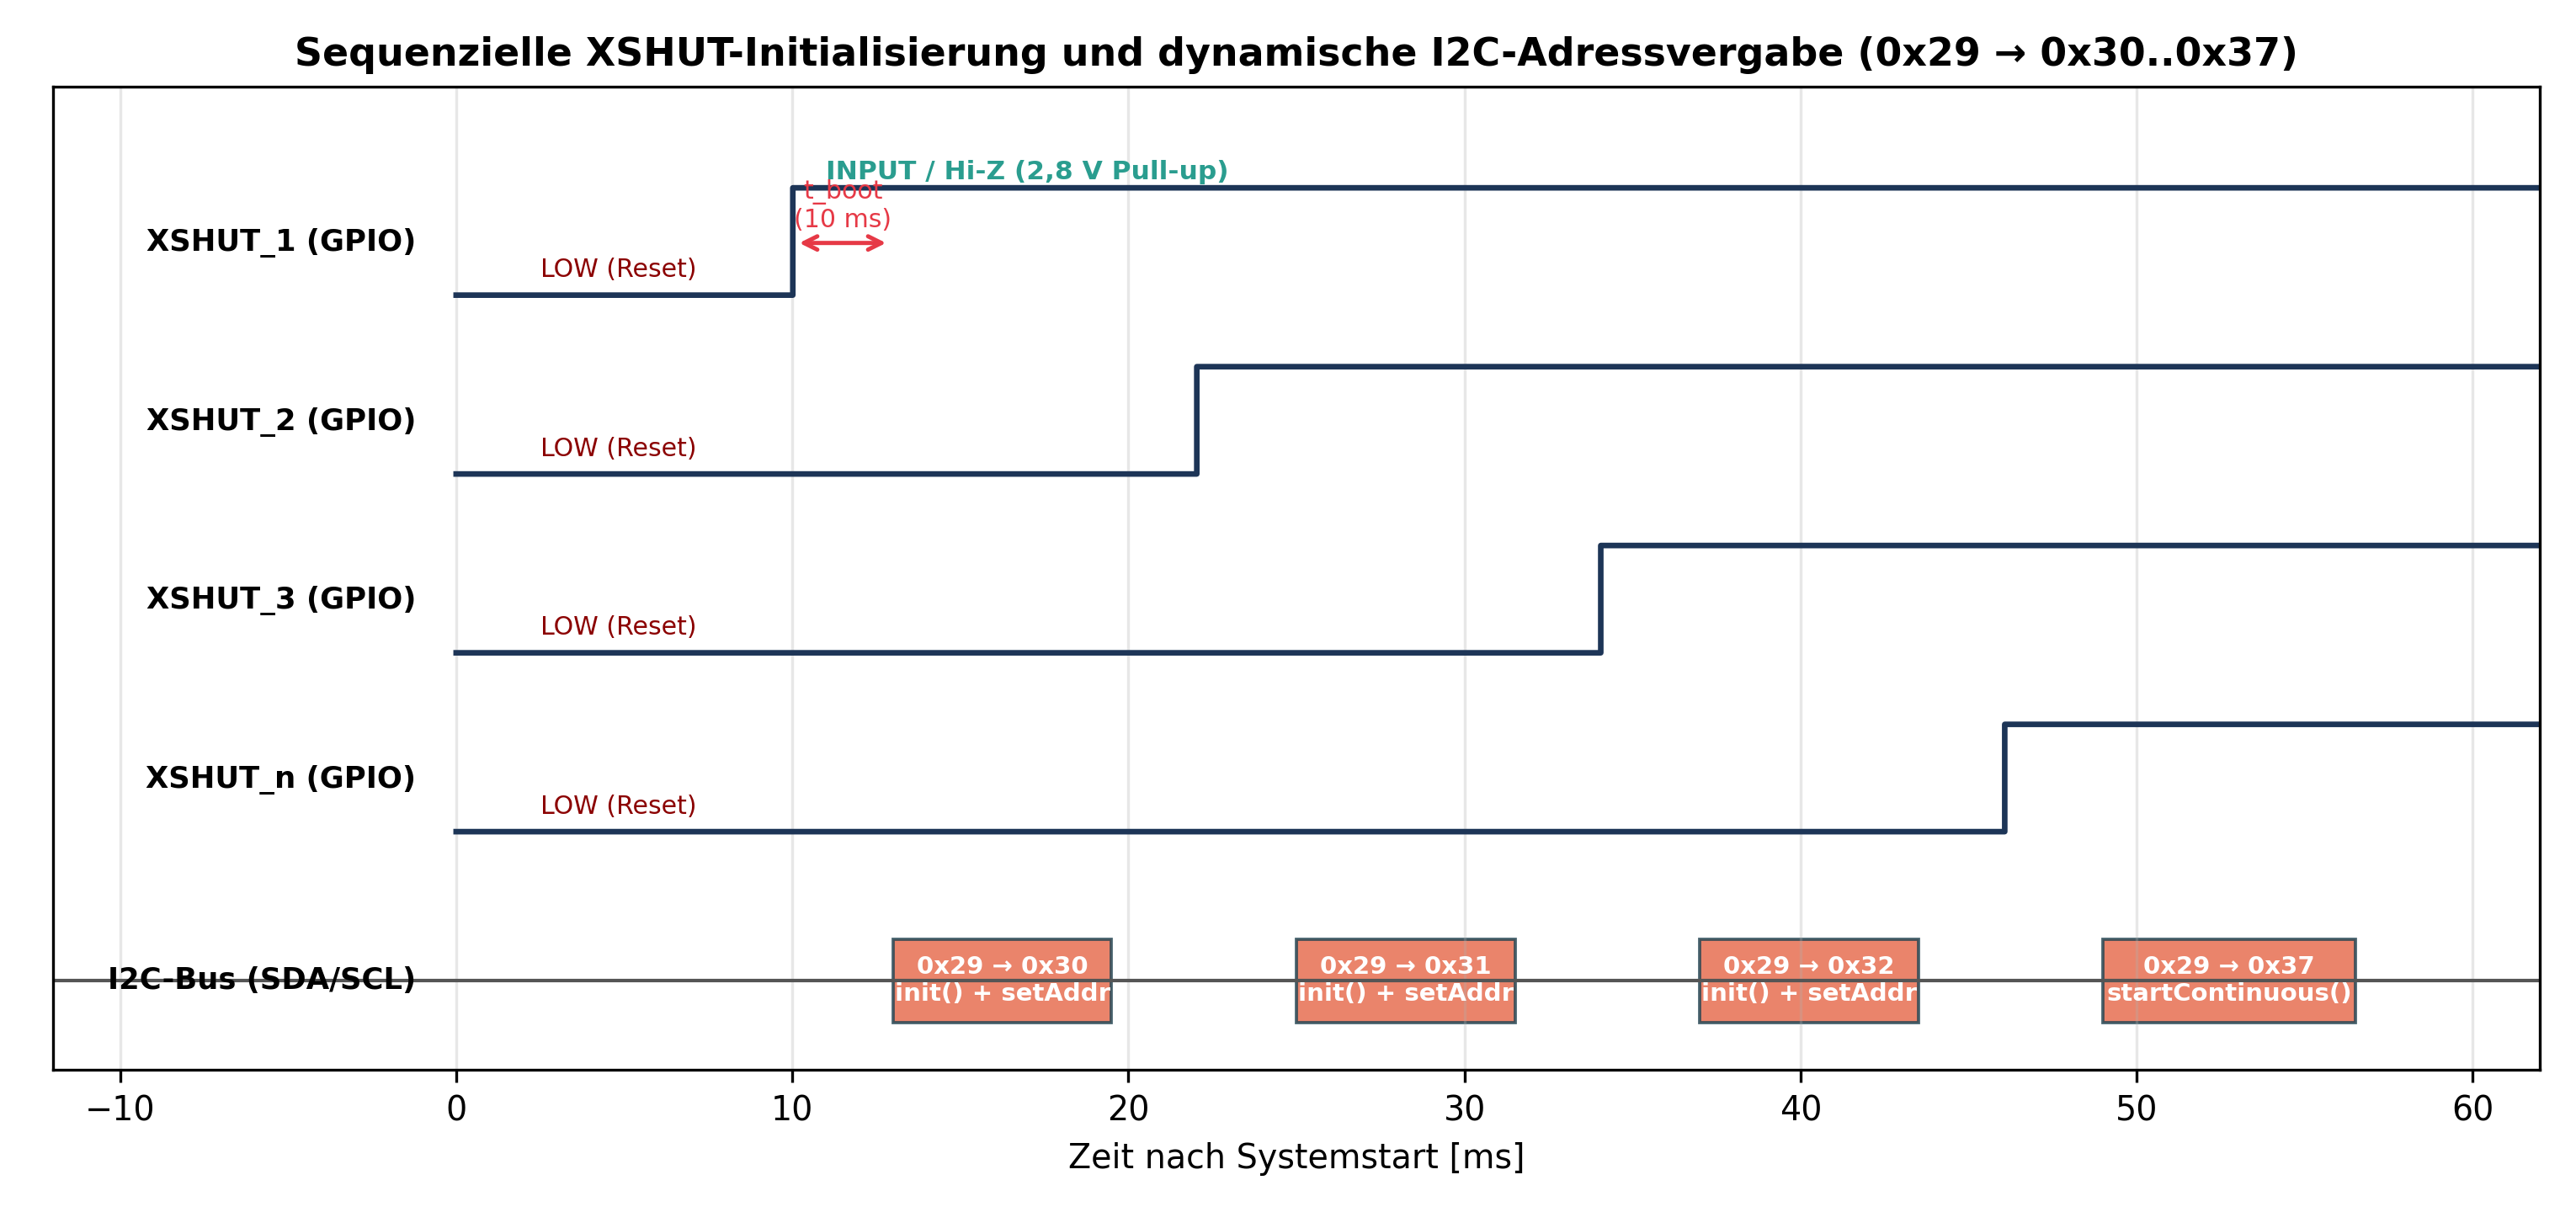
\includegraphics[width=0.96\textwidth]{figures/fig_xshut_i2c_timing.png}
  \caption{Zeitlicher Ablauf der sequenziellen XSHUT-Bootsequenz und dynamischen I\textsuperscript{2}C-Adressvergabe (\texttt{0x29} $\rightarrow$ \texttt{0x30}--\texttt{0x37}).}
  \label{fig:xshut_timing}
\end{figure}

\subsection{Elektrische Besonderheit: Hi-Z-Freigabe statt 3,3-V-High-Pegel}
Ein wichtiges Schaltungsdetail der violetten \emph{VL53L0/1XV2}-Module betrifft den Spannungspegel am \texttt{XSHUT}-Pin: Intern arbeitet der Sensor-IC mit \qty{2,8}{\volt} aus einem On-Board-LDO. Schaltet der ESP32-S3 den \texttt{XSHUT}-GPIO aktiv als \texttt{OUTPUT HIGH} auf \qty{3,3}{\volt}, fließt über die internen Schutzdioden ein unerwünschter Rückstrom in die \qty{2,8}{\volt}-Domäne. In unserer Firmware (Listing~\ref{lst:xshut_main}) wird dieses Problem sauber gelöst:
\begin{enumerate}
  \item Zu Beginn werden alle \texttt{XSHUT}-Pins als \texttt{GPIO\_MODE\_OUTPUT} auf \texttt{LOW} (\qty{0}{\volt}) gezogen, wodurch alle Sensoren sicher im Hardware-Reset verharren.
  \item Anschließend wird für jeden Sensor $i$ der zugehörige Pin auf \texttt{GPIO\_MODE\_INPUT} (hochohmig / \emph{Hi-Z}) umgeschaltet. Der auf dem Sensormodul vorhandene interne Pull-up-Widerstand zieht \texttt{XSHUT} nun exakt auf seine eigene \qty{2,8}{\volt}-Betriebsspannung.
  \item Nach einer Boot-Wartezeit von \qty{10}{\milli\second} (Datenblatt-Minimum $t_{\mathrm{boot}} = \qty{1,2}{\milli\second}$) antwortet ausschließlich Sensor $i$ auf der Default-Adresse \texttt{0x29}. Die Methode \texttt{setAddress(ADDRESSES[i])} schreibt die neue eindeutige Adresse (\texttt{0x30}, \texttt{0x31}, \dots) ins Register und startet den kontinuierlichen Messbetrieb (\texttt{startContinuous()}).
\end{enumerate}

\subsection{Reale ESP-IDF-Implementierung am Labor-Prüfstand}
Für die schrittweise Inbetriebnahme und Treibervalidierung wurde im Branch \texttt{Main\_code} (\texttt{main/main.cpp}) ein lauffähiger 4-Sensor-Prüfstand unter ESP-IDF mit portierter Pololu-C++-Bibliothek (\texttt{components/vl53l0x/VL53L0X.cpp}) aufgebaut \cite{PololuVL53L0X}. Listing~\ref{lst:xshut_main} zeigt den real getesteten Initialisierungs- und Auslesecode, der für das Gesamtfahrzeug direkt durch Erweiterung der Arrays \texttt{XSHUT\_PINS} und \texttt{ADDRESSES} auf \texttt{NUM\_SENSORS = 8} skaliert wird.

\begin{lstlisting}[language=C++,caption={Reale ESP-IDF-Implementierung der XSHUT-Initialisierung und kontinuierlichen Distanzmessung aus \texttt{main/main.cpp} (Branch \texttt{Main\_code}).},label={lst:xshut_main}]
static const int NUM_SENSORS = 4; // Gesamtfahrzeug: 8 (0x30 .. 0x37)
static const gpio_num_t XSHUT_PINS[NUM_SENSORS] = {
    GPIO_NUM_27, GPIO_NUM_26, GPIO_NUM_25, GPIO_NUM_33
};
static const uint8_t ADDRESSES[NUM_SENSORS] = {0x30, 0x31, 0x32, 0x33};

static void initI2c() {
    i2c_config_t conf = {};
    conf.mode             = I2C_MODE_MASTER;
    conf.sda_io_num       = GPIO_NUM_21;
    conf.scl_io_num       = GPIO_NUM_22;
    conf.sda_pullup_en    = GPIO_PULLUP_ENABLE;
    conf.scl_pullup_en    = GPIO_PULLUP_ENABLE;
    conf.master.clk_speed = 100000; // 100 kHz Standard-Mode
    ESP_ERROR_CHECK(i2c_param_config(I2C_NUM_0, &conf));
    ESP_ERROR_CHECK(i2c_driver_install(I2C_NUM_0, conf.mode, 0, 0, 0));
}

static void setup() {
    initI2c();
    // 1. Alle Sensoren ueber XSHUT in Hardware-Reset halten
    for (int i = 0; i < NUM_SENSORS; i++) {
        gpio_reset_pin(XSHUT_PINS[i]);
        gpio_set_direction(XSHUT_PINS[i], GPIO_MODE_OUTPUT);
        gpio_set_level(XSHUT_PINS[i], 0);
    }
    vTaskDelay(pdMS_TO_TICKS(10));

    // 2. Nacheinander via Hi-Z (INPUT) aufwecken und Adresse zuweisen
    for (int i = 0; i < NUM_SENSORS; i++) {
        gpio_set_direction(XSHUT_PINS[i], GPIO_MODE_INPUT);
        vTaskDelay(pdMS_TO_TICKS(10));
        sensors[i].setPort(I2C_NUM_0);
        sensors[i].setTimeout(500);
        if (sensors[i].init()) {
            sensors[i].setAddress(ADDRESSES[i]);
            sensors[i].startContinuous();
            sensorOk[i] = true;
        }
    }
}
\end{lstlisting}

\subsection{I\textsuperscript{2}C-Zeitbudget-Analyse für den 8-Sensor-Betrieb}
\label{sec:i2c_zeitbudget}
Da alle acht \emph{VL53L0X}-Sensoren sowie die \emph{LSM6DSV}-IMU denselben I\textsuperscript{2}C-Bus nutzen, muss rechnerisch geprüft werden, ob das serielle Auslesen innerhalb der \qty{40}{\milli\second}-Periode des \texttt{LidarImuTask} zuverlässig gelingt. Im kontinuierlichen Messbetrieb (\texttt{startContinuous()}) ermittelt jeder Sensor seine Distanz autonom im Hintergrund. Das Auslesen eines 16-Bit-Ergebnisregisters (\texttt{RESULT\_RANGE\_STATUS + 10}) samt Status-Abfrage und Interrupt-Quittierung umfasst rund 6~Byte pro Sensor (inkl. Start-, Adress-, Register- und Stopp-Bits ca. 60~Taktzyklen). Für alle acht Sensoren ergibt sich damit eine reine Busbelegungszeit von:
\begin{align}
  t_{\mathrm{Bus,100k}} &= 8 \cdot \frac{60}{\qty{100}{\kilo\hertz}} = \qty{4,80}{\milli\second} \quad (\text{12\,\% Buslast bei }\qty{40}{\milli\second}\text{ Zyklus}) \label{eq:i2c_t100} \\
  t_{\mathrm{Bus,400k}} &= 8 \cdot \frac{60}{\qty{400}{\kilo\hertz}} = \qty{1,20}{\milli\second} \quad (\text{3\,\% Buslast bei }\qty{40}{\milli\second}\text{ Zyklus}) \label{eq:i2c_t400}
\end{align}
Selbst im konservativen \qty{100}{\kilo\hertz}-Standard-Mode verbleiben über \qty{34}{\milli\second} Reserve pro Zyklus für die IMU-Abfrage und die digitale Filterung.

% ==============================================================================
\section{Messwertvorverarbeitung und digitale Filterung}
\label{sec:filterung}
% ==============================================================================
Rohdaten von \gls{tof}-Sensoren enthalten im praktischen Laborbetrieb zwei typische Störungsarten: erstens sporadische Ausreißer (\emph{Spikes}) durch Spiegelreflexionen oder ungültige Messungen (\texttt{d >= 8190} bzw. \texttt{timeoutOccurred()}), und zweitens statistisches Messrauschen im Bereich von $\pm \qtyrange{3}{8}{\milli\meter}$. Würden ungefilterte Rohwerte direkt in die Flankenerkennung der Parklückensuche eingespeist, könnte ein einziger Fehlimpuls das vorzeitige Ende einer Parklücke vortäuschen.

Aus diesem Grund durchläuft jeder Sensorkanal eine zweistufige Filterkette:
\begin{enumerate}
  \item \textbf{Plausibilitätsprüfung und 3-Punkte-Medianfilter:} Werte außerhalb des gültigen Messbereichs ($d < \qty{20}{\milli\meter}$ oder $d \ge \qty{8190}{\milli\meter}$) werden auf den Maximalwert $d_{\max} = \qty{1500}{\milli\meter}$ (freier Raum) geklemmt bzw. bei Timeout als ungültig markiert. Der anschließende Medianfilter über die letzten drei Messwerte
  \begin{equation}
    d_{\mathrm{med}}[k] = \mathrm{median}\bigl(d_{\mathrm{roh}}[k],\, d_{\mathrm{roh}}[k-1],\, d_{\mathrm{roh}}[k-2]\bigr)
    \label{eq:median}
  \end{equation}
  eliminiert einzelne Ausreißer vollständig, ohne echte Kantenübergänge (wie den Beginn einer Parklücke) zu verschmieren.
  \item \textbf{Exponentiell gewichteter gleitender Mittelwert (\gls{ema}):} Zur Glättung des verbleibenden Grundrauschens folgt ein rekursiver Tiefpass erster Ordnung:
  \begin{equation}
    d_{\mathrm{filt}}[k] = \alpha \cdot d_{\mathrm{med}}[k] + (1 - \alpha) \cdot d_{\mathrm{filt}}[k-1], \qquad \alpha \in (0, 1]
    \label{eq:ema}
  \end{equation}
  Mit $\alpha = 0{,}35$ bei einer Messrate von \qty{25}{\hertz} ($T_{\mathrm{LiDAR}} = \qty{40}{\milli\second}$) ergibt sich eine effektive Filterzeitkonstante von ca. \qty{95}{\milli\second} -- schnell genug für scharfe Parklückenkanten bei einer Suchgeschwindigkeit von $v_{\mathrm{Scan}} = \qty{0,25}{\meter\per\second}$ (entspricht \qty{24}{\milli\meter} Wegstrecke), aber ruhig genug für eine stabile Abstandsregelung.
\end{enumerate}

% ==============================================================================
\section{Geometrische Parklückenerkennung}
\label{sec:parkluecke}
% ==============================================================================
Die Erkennung einer geeigneten Längsparklücke auf der rechten Fahrzeugseite basiert auf der zeitlichen Kopplung des seitlichen LiDAR-Sensors \texttt{3e} ($0^\circ$, rechts) mit der zurückgelegten Wegstrecke $s(t)$ aus der Hinterachs-Odometrie (Abbildung~\ref{fig:parking_geom}).

\begin{figure}[htbp]
  \centering
  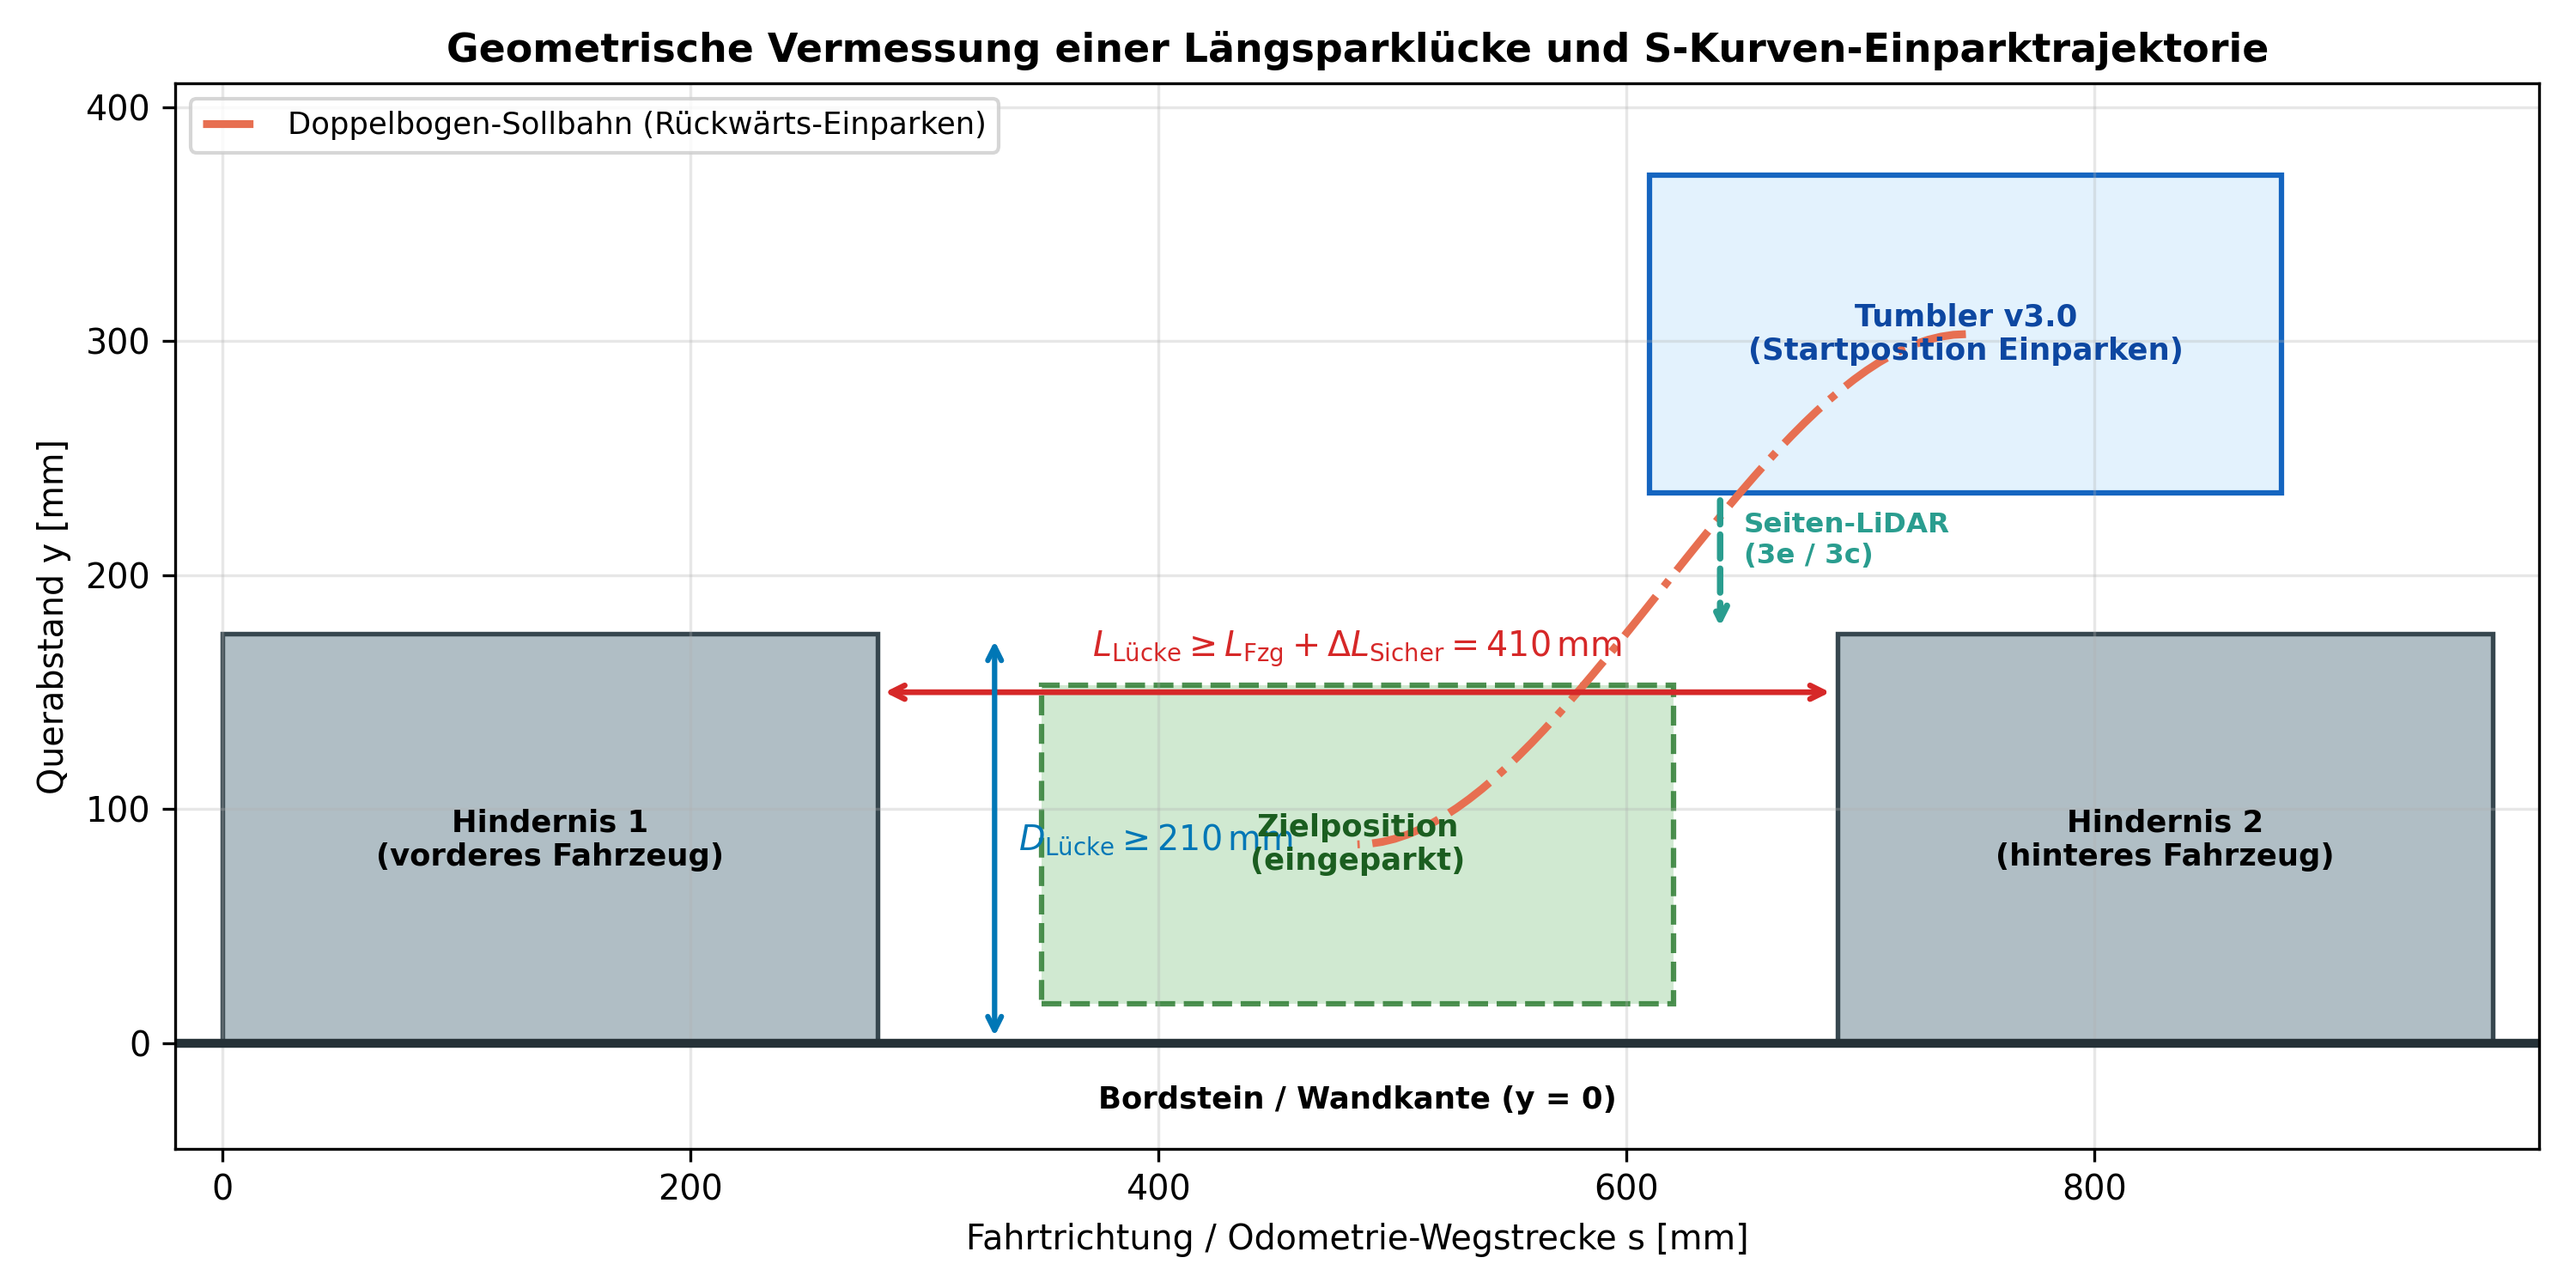
\includegraphics[width=0.98\textwidth]{figures/fig_parking_geometry.png}
  \caption{Geometrische Vermessung einer Längsparklücke über Seiten-LiDAR (\texttt{3e}) und Odometrie-Wegstrecke $s$ sowie Solltrajektorie für das Rückwärts-Einparken.}
  \label{fig:parking_geom}
\end{figure}

\subsection{Kriterien für eine befahrbare Längsparklücke}
Das Fahrzeug besitzt in Revision~v10.0 eine Gesamtlänge von $L_{\mathrm{Fzg}} = \qty{270,4}{\milli\meter}$ und eine Breite über die Antriebsräder von $B_{\mathrm{Fzg}} = \qty{184,0}{\milli\meter}$. Damit ein sicheres Rückwärts-Einparken ohne Touchieren der begrenzenden Hindernisse möglich ist, muss eine erkannte Lücke zwei geometrische Bedingungen gleichzeitig erfüllen:
\begin{align}
  L_{\mathrm{L\ddot{u}cke}} &= s_{\mathrm{Ende}} - s_{\mathrm{Start}} \ge L_{\mathrm{Fzg}} + \Delta L_{\mathrm{Sicher}} = \qty{270,4}{\milli\meter} + \qty{139,6}{\milli\meter} = \qty{410}{\milli\meter} \label{eq:gap_len} \\
  D_{\mathrm{L\ddot{u}cke}} &= d_{\mathrm{3e,min,L\ddot{u}cke}} - d_{\mathrm{Wand,ref}} \ge B_{\mathrm{Fzg}} + \Delta B_{\mathrm{Sicher}} = \qty{184,0}{\milli\meter} + \qty{26,0}{\milli\meter} = \qty{210}{\milli\meter} \label{eq:gap_depth}
\end{align}
Um Flattern an der Hinderniskante zu vermeiden, arbeitet die Kanten-Erkennung mit einer Hysterese:
\begin{itemize}
  \item \textbf{Eintritt in mögliche Lücke (\emph{Rising Edge}):} Wenn $d_{\mathrm{3e,filt}} > d_{\mathrm{Wand,ref}} + \qty{180}{\milli\meter}$, wird der aktuelle Odometriestand als $s_{\mathrm{Start}}$ gespeichert und die minimale gemessene Lückentiefe $D_{\mathrm{min}}$ laufend mitgeführt.
  \item \textbf{Ende der Lücke (\emph{Falling Edge}):} Fällt $d_{\mathrm{3e,filt}}$ wieder unter $d_{\mathrm{Wand,ref}} + \qty{120}{\milli\meter}$, wird $s_{\mathrm{Ende}}$ gespeichert. Sind beide Bedingungen \eqref{eq:gap_len} und \eqref{eq:gap_depth} erfüllt, meldet das Sensorik-Modul eine gültige Parklücke an die Einpark-FSM (Kapitel~\ref{sec:einpark_fsm}).
\end{itemize}

\begin{lstlisting}[language=C++,caption={Zweistufiger Median-3- und EMA-Distanzfilter sowie Hysterese-Parklückendetektor (C++).},label={lst:gap_filter}]
struct LidarFilter {
    uint16_t ring[3] = {1500, 1500, 1500};
    uint8_t  idx     = 0;
    float    ema     = 1500.0f;

    float update(uint16_t rawMm, bool timeout) {
        uint16_t clamped = (timeout || rawMm >= 8190 || rawMm < 20) ? 1500 : rawMm;
        ring[idx] = clamped;
        idx = (idx + 1) % 3;
        // 3-Punkte-Median ohne dynamische Speicherallokation
        uint16_t a = ring[0], b = ring[1], c = ring[2];
        uint16_t med = (a > b) ? ((b > c) ? b : ((a > c) ? c : a))
                               : ((a > c) ? a : ((b > c) ? c : b));
        ema = 0.35f * static_cast<float>(med) + 0.65f * ema;
        return ema;
    }
};

struct GapDetector {
    bool  inGap    = false;
    float sStartMm = 0.0f;
    float minDepth = 1500.0f;
    float wallRef  = 140.0f; // Referenzabstand zur geparkten Fahrzeugreihe

    bool update(float dRightMm, float odoSMm, float &foundLenMm) {
        if (!inGap && dRightMm > wallRef + 180.0f) {
            inGap = true;
            sStartMm = odoSMm;
            minDepth = dRightMm - wallRef;
        } else if (inGap) {
            float curDepth = dRightMm - wallRef;
            if (curDepth < minDepth) minDepth = curDepth;
            if (dRightMm < wallRef + 120.0f) {
                inGap = false;
                float len = odoSMm - sStartMm;
                if (len >= 410.0f && minDepth >= 210.0f) {
                    foundLenMm = len;
                    return true; // Gueltige Laengsparkluecke bestaetigt!
                }
            }
        }
        return false;
    }
};
\end{lstlisting}

% ==============================================================================
\section{Optische Linienerkennung und Kalibrierung}
\label{sec:linienerkennung}
% ==============================================================================
Für die Spurführung während der Anfahrt werden die sechs analogen Kanäle \texttt{LS1}--\texttt{LS6} der Liniensensor-Platine (Kapitel~\ref{sec:liniensensor_pcb}) über \texttt{ADC1\_CH3} bis \texttt{ADC1\_CH9} mit \qty{100}{\hertz} abgetastet. Da Umgebungslicht, Bodenreflexion und Bauteiltoleranzen der einzelnen \emph{CNY70} variieren, durchläuft das Fahrzeug vor der Fahrt eine Zweipunkt-Kalibrierung über der hellen Fahrbahn ($U_{\mathrm{wei\ss},i}$) und der schwarzen Linie ($U_{\mathrm{schwarz},i}$).

Jeder Rohmesswert $U_i$ wird anschließend auf einen normierten Schwärzungsgrad $n_i \in [0, 1]$ abgebildet (wobei $n_i = 1$ einer dunklen Linie entspricht, da $U_{\mathrm{schwarz},i} > U_{\mathrm{wei\ss},i}$):
\begin{equation}
  n_i = \mathrm{clamp}_{[0, 1]}\!\left(\frac{U_i - U_{\mathrm{wei\ss},i}}{U_{\mathrm{schwarz},i} - U_{\mathrm{wei\ss},i}}\right)
  \label{eq:ls_norm}
\end{equation}
Mit den realen mechanischen Sensorpositionen $x_i \in \{-25, -15, -5, +5, +15, +25\}\,\mathrm{mm}$ (\qty{10}{\milli\meter}-Raster symmetrisch zur Fahrzeuglängsachse) ergibt sich die stufenlose seitliche Linienablage $e_{\mathrm{Linie}}$ in Millimetern durch gewichtete Schwerpunktberechnung:
\begin{equation}
  e_{\mathrm{Linie}} = \frac{\sum_{i=1}^{6} x_i \cdot n_i}{\sum_{i=1}^{6} n_i}, \qquad \text{für } \sum_{i=1}^{6} n_i > \varepsilon_{\min}
  \label{eq:ls_centroid}
\end{equation}
Unterschreitet die Summe $\sum n_i$ den Schwellwert $\varepsilon_{\min} = 0{,}35$, erkennt die Firmware einen Linienverlust und hält entweder die letzte bekannte Suchrichtung oder schaltet sicher in den Stoppzustand. Umgekehrt signalisiert $\sum n_i > 4{,}8$ eine querliegende Stopp- oder Startmarkierung auf dem Testparcours.

\chapterauthor{Adem Merdzic}
\chapter{Robotik-Software und Regelungstechnik}
\label{chap:software_regelung}

\section{Firmware-Architektur auf dem ESP32-S3}
\label{sec:firmware_architektur}

Die Steuerungssoftware baut auf der bestehenden \emph{ESP-IDF}- bzw. \emph{RtEnv}-Projektstruktur der HTL~BULME auf \cite{Kloeckl2026}, wird jedoch vollständig an die geänderte Hardware der Hauptplatine (\emph{ESP32-S3-WROOM-1}, integrierte \emph{TB67H450FNG}-Treiber, \emph{LSM6DSV}-IMU) sowie das 8-fach-\gls{lidar}-Array angepasst.

Um zeitkritische Regelungsaufgaben (Motor-\gls{pwm}, Encoder-Auswertung, IMU-Integration) sauber von der langsameren Umfelderfassung und Ablaufsteuerung zu entkoppeln, gliedert sich die Firmware unter FreeRTOS in modulare Tasks:
\begin{itemize}
  \item \textbf{Sensor-Task:} Zyklisches Auslesen der acht \emph{VL53L0/1XV2}-Sensoren, der \gls{imu} (\emph{LSM6DSV}) sowie bei Bedarf des Liniensensors (\emph{CNY70}-Array).
  \item \textbf{Regelungs-Task:} Berechnung der Soll-/Ist-Drehzahlen und des Gierwinkels $\psi(t)$ sowie Ausgabe der \gls{pwm}-Tastverhältnisse an \texttt{U6} und \texttt{U7}.
  \item \textbf{Steuerungs-Task (Zustandsautomat):} Auswertung der Parklückenkandidaten und Koordination der einzelnen Fahrphasen.
  \item \textbf{Telemetrie-Task:} Übertragung von Zustands- und Messdaten über USB-C bzw. \emph{SvVis} zur Diagnose \cite{Kloeckl2026}.
\end{itemize}

\todo[inline]{[TODO: Konkrete Task-Prioritäten, Zykluszeiten (ms) und GPIO-Zuordnungen aus der finalen ESP-IDF-Konfiguration nachtragen.]}

\section{Zustandsautomat für das autonome Einparken}
\label{sec:zustandsautomat}

Der gesamte Einparkvorgang wird über einen deterministischen endlichen Zustandsautomaten (Finite State Machine, FSM) abgebildet, sodass zu jedem Zeitpunkt ein klar definiertes Fahrverhalten inklusive sicherer Abbruchbedingungen bei unerwarteten Hindernissen vorliegt. Abbildung~\ref{fig:fsm_einparken} zeigt den grundlegenden Ablauf.

\begin{figure}[htbp]
  \centering
  \begin{tikzpicture}[
    node distance=0.85cm and 1.2cm,
    state/.style={rectangle, draw=black!80, fill=blue!5, rounded corners=3pt, minimum width=3.4cm, minimum height=0.8cm, align=center, font=\small},
    err/.style={rectangle, draw=red!75!black, fill=red!6, rounded corners=3pt, minimum width=3.0cm, minimum height=0.8cm, align=center, font=\small},
    arrow/.style={->, >=stealth, thick}
  ]
    \node[state] (init) {\textbf{IDLE / INIT}\\Sensoren \& IMU kalibrieren};
    \node[state, below=of init] (scan) {\textbf{SCAN}\\Vorbeifahrt \& Lückensuche};
    \node[state, below=of scan] (align) {\textbf{ALIGN}\\Positionierung vor Lücke};
    \node[state, below=of align] (park) {\textbf{PARK\_MANEUVER}\\Geregeltes Einparken};
    \node[state, below=of park] (done) {\textbf{PARKED}\\Stopp \& Status-LED grün};
    \node[err, right=2.2cm of park] (abort) {\textbf{SAFETY\_STOP}\\Kollisionsschutz};

    \draw[arrow] (init) -- (scan);
    \draw[arrow] (scan) -- node[right, font=\scriptsize]{Lücke gültig} (align);
    \draw[arrow] (align) -- node[right, font=\scriptsize]{Startpose erreicht} (park);
    \draw[arrow] (park) -- node[right, font=\scriptsize]{Endpose erreicht} (done);
    \draw[arrow] (scan) -| node[above, near start, font=\scriptsize]{Not-Aus} (abort);
    \draw[arrow] (align) -| (abort);
    \draw[arrow] (park) -- node[above, font=\scriptsize]{$d < d_{\text{min}}$} (abort);
  \end{tikzpicture}
  \caption{Zustandsautomat (FSM) der übergeordneten Einparksteuerung.}
  \label{fig:fsm_einparken}
\end{figure}

Die hinteren drei \gls{lidar}-Sensoren (\texttt{3f}, \texttt{3g}, \texttt{3h}) übernehmen im Zustand \texttt{PARK\_MANEUVER} die aktive Rückraumüberwachung: Unterschreitet ein Sensor den definierten Sicherheitsabstand $d_{\text{min}}$, wird sofort in \texttt{SAFETY\_STOP} gewechselt und beide Motortreiber werden aktiv gebremst.

\section{Antriebs-, Geschwindigkeits- und Lageregelung}
\label{sec:regelung}

Da das Fahrzeug über zwei unabhängig angetriebene Räder (Differentialantrieb) verfügt, werden sowohl die Translationsgeschwindigkeit $v$ als auch die Kurvenfahrt (Drehrate $\omega_z$ bzw. Gierwinkel $\psi$) über die Differenz der beiden Motordrehzahlen geregelt. Für die Geschwindigkeits- und Winkelregelung kommt ein zeitdiskreter PID-Regler zum Einsatz:
\begin{equation}
  u[k] = K_P\,e[k] + K_I\,T_s \sum_{j=0}^{k} e[j] + K_D\,\frac{e[k] - e[k-1]}{T_s}
  \label{eq:pid_diskret}
\end{equation}
mit der Regelabweichung $e[k] = w[k] - y[k]$ und der Abtastzeit $T_s$. Während der geraden Vorbeifahrt (\texttt{SCAN}) hält ein unterlagerter Winkelregler den Gierwinkel $\psi$ mittels \gls{imu}-Rückführung konstant, sodass schräge Drifts nicht die Lückenvermessung verfälschen.

\todo[inline]{[TODO: Ermittelte Reglerparameter (Kp, Ki, Kd), Abtastzeit Ts sowie kommentierte Code-Auszüge der Motoransteuerung und Zustandsmaschine aus dem fertigen Software-Repository ergänzen.]}

\chapterauthor{Adem Merdzic, Rami Muarrawi, Christopher Schieszler}
\chapter{Inbetriebnahme, Systemvalidierung und Fazit}
\label{chap:validierung_fazit}

\section{Digitale CAD- und Kollisionsvalidierung (DMU-Audit)}
\label{sec:dmu_audit}

Vor der physischen Fertigung des Unibody-Chassis wurde das gesamte Fahrzeug in Revision~v9.0 einer automatisierten, paarweisen BRep-Volumenkollisionsprüfung über alle \num{121} Einzelkörper (Chassis, Hauptplatine mit sämtlichen SMD-Bauteilen und Steckverbindern, Liniensensor inkl. \emph{CNY70}-Array, 8x \emph{VL53L0/1XV2}-Platinen, 16x M2x6-Schrauben, 4x M3x8-Hauptplatinenschrauben mit Messing-Gewindeeinsätzen, 4x M3x14-Liniensensorschrauben mit Muttern, 8x M4x10-Motorschrauben, Motoren, Räder, 2S-Akkupack inkl. XT30/Balancer sowie 9x 24-mm-Steckerdummies und 3D-Kabelbaum) unterzogen.

\begin{table}[htbp]
  \centering
  \caption{Zusammenfassung der digitalen Konstruktions- und Kollisionsprüfung (Revision~v9.0).}
  \label{tab:dmu_ergebnis}
  \begin{tabular}{@{}lll@{}}
    \toprule
    \textbf{Prüfkriterium} & \textbf{Zielvorgabe} & \textbf{Ergebnis (Rev.~v9.0)} \\
    \midrule
    BRep-Kollisionsprüfung (121 Körper) & \SI{0.000}{\milli\metre\cubed} Kollision & 0 Kollisionen (\SI{0.000}{\milli\metre\cubed}) \\
    Chassis-Festkörperstruktur & Einteiliger Monolith & 1 Solid (\SI{218.8}{\centi\metre\cubed}, ca.~\SI{271}{\gram}) \\
    Mindestwandstärke (Base / Wand / Pod-Dach) & $\ge \SI{2.5}{\milli\metre}$ & \SI{4.0}{\milli\metre} / \SI{3.5}{\milli\metre} / \SIrange{3.85}{4.30}{\milli\metre} \\
    Restwandstärke um Schraubendome & $\ge \SI{2.0}{\milli\metre}$ & \SI{3.30}{\milli\metre} (M3) bzw. $\ge \SI{2.02}{\milli\metre}$ (M2) \\
    Akkufach-Toleranz ($72\times 39{,}5\times 19{,}5\,\si{\milli\metre}$) & $\ge +\SI{1.5}{\milli\metre}$ umlaufend & $+\SI{2.0}{\milli\metre}$ ($X,Z$) / $+\SI{3.0}{\milli\metre}$ ($Y$) \\
    Crash-Sicherheitsfaktor ($\SI{5}{\kilo\metre\per\hour}$ / $\SI{9}{\kilo\metre\per\hour}$) & $\text{SF} \ge 3{,}0$ & $\text{SF} = 37{,}0$ / $\text{SF} = 11{,}4$ \\
    \bottomrule
  \end{tabular}
\end{table}

\section{Hardware-Inbetriebnahme und Messreihen}
\label{sec:inbetriebnahme_tests}

Nach der Bestückung der Haupt- und Liniensensor-Platine sowie dem 3D-Druck des Gehäuses folgen die stufenweisen Hardware- und Systemtests am realen Fahrzeug:
\begin{enumerate}
  \item \textbf{Stromversorgungstest:} Überprüfung der Leerlauf- und Lastspannungen (\SI{3.3}{\volt} und \SI{5.0}{\volt}) sowie Stromaufnahme im Ruhezustand.
  \item \textbf{Kommunikationstest:} USB-C-Verbindung zum \emph{ESP32-S3}, Erkennung aller acht I\textsuperscript{2}C-Adressen der \gls{lidar}-Sensoren und Auslesen der \emph{LSM6DSV}-Rohdaten.
  \item \textbf{Sensor-Genauigkeitstest:} Vergleich der gefilterten \emph{VL53L0/1XV2}-Distanzen mit Referenzabständen im Nahbereich (\SIrange{50}{1000}{\milli\metre}).
  \item \textbf{Einparkversuch:} Reproduzierbarkeit und Kollisionsfreiheit des autonomen Einparkmanövers in definierten Testlücken.
\end{enumerate}

\todo[inline]{[TODO: Gemessene Spannungs-/Oszilloskopwerte, I2C-Scan-Protokolle, Sensor-Fehlerkurven, reale Fotos der bestückten Platinen sowie Ergebnisse der Einparkversuche nach Durchführung im Labor einfügen.]}

\section{Fazit und Ausblick}
\label{sec:fazit}

Mit dem Abschluss des Elektronik-Redesigns und des mechanischen Unibody-Chassis (Revision~v9.0) wurden die zentralen Schwachstellen der Vorgängerplattform systematisch behoben. Durch die direkte Integration von Motortreibern und \gls{imu} auf die Hauptplatine entfallen fehleranfällige Steckmodule, während die acht geschützt verbauten \gls{lidar}-Sensoren eine lückenlose 360\textdegree-Umfelderfassung ermöglichen. Die digitale BRep-Validierung bestätigt die vollständige Kollisionsfreiheit und Montierbarkeit aller 121~Einzelkomponenten.

Nach Abschluss der laufenden Software-Integration und der praktischen Einparktests bietet die Plattform eine stabile Grundlage für weiterführende Projekte im Unterricht -- etwa für erweiterte Pfadplanungsalgorithmen (z.\,B. Rückwärts- und Querparken bei schrägen Hindernissen) oder die Einbindung von Funk-Telemetrie zur Live-Visualisierung der LiDAR-Umfeldkarte.


\appendix
\chapterauthor{Adem Merdzic, Rami Muarrawi, Christopher Schieszler}
\chapter{Anhang}
\label{chap:anhang}

\section{Übersicht der CAD- und Konstruktionsdateien}
\label{sec:anhang_cad}

Sämtliche Produktions-, Baugruppen- und Skriptdateien der finalen Revision~v9.0 sind im Projekt-Repository unter \texttt{3D\_Design-Modelling/} abgelegt (Tabelle~\ref{tab:anhang_dateien}).

\begin{table}[htbp]
  \centering
  \caption{Zentrale CAD- und Fertigungsdateien der Revision~v9.0 im Repository.}
  \label{tab:anhang_dateien}
  \begin{tabular}{@{}ll@{}}
    \toprule
    \textbf{Dateiname} & \textbf{Beschreibung} \\
    \midrule
    \texttt{...\_v3\_LiDar\_V2\_integrated.step} & Monolithisches Unibody-Chassis (STEP, BRep) \\
    \texttt{...\_v3\_LiDar\_V2\_integrated.stl} & Druckfertiges Unibody-Chassis (STL, 0\,g Support) \\
    \texttt{...\_v3\_DMU\_Assembly.step} & Gesamtbaugruppe mit allen 121 Einzelkörpern (STEP) \\
    \texttt{...\_v3\_DMU\_Assembly.py} & Fusion-360-API-Skript inklusive Interference Audit \\
    \texttt{v9\_Final\_DMU\_Master\_Preview.png} & Vierseiten-Übersichtsrendering des Final-DMU \\
    \bottomrule
  \end{tabular}
\end{table}

\section{Schaltpläne und Stücklisten}
\label{sec:anhang_schaltplaene}

\todo[inline]{[TODO: Exportierte PDF-Schaltpläne von Tumbler2\_Redesign und Liniensensor sowie vollständige Bestückungslisten (BOM) als Anhangsseiten einbinden.]}


\newpage
\bibliography{literatur-bib}
\nocite{*}

\newpage
\glsaddall
\printglossary[title={Abkürzungs- und Glossarverzeichnis}]

\end{document}
